% ==============================================================================
% Copyright (c) 2017 [Georg R. Pollak]  
% ==============================================================================
% ------------------------------------------------------------------------------

  % Permission is hereby granted, free of charge, to any person obtaining a copy
  % of this software and associated documentation files (the "Software"), to deal
  % in the Software without restriction, including without limitation the rights
  % to use, copy, modify, merge, publish, distribute, sublicense, and/or sell
  % copies of the Software, and to permit persons to whom the Software is
  % furnished to do so, subject to the following conditions:

  % The above copyright notice, the creator of the formuary package G.R. Pollak
  % and this permission notice shall be included in all copies or substantial portions of the Software.

% ==============================================================================
% End
% ==============================================================================
% ------------------------------------------------------------------------------

% Document class
% ------------------------------------------------------------------------------
\documentclass[fourColumns]{formularyETH/formularyETH}
% formuaryETH packages
% ------------------------------------------------------------------------------
\usepackage{formularyETH/formularyETH_GeneralPackages}
\usepackage{formularyETH/formularyETH_underline}
\usepackage{formularyETH/extern/formularyETH_scientific}
\usepackage{formularyETH/extern/formularyETH_tikz}
\usepackage{formularyETH/extern/formularyETH_algorithms}
% Other very usefull packages
% ------------------------------------------------------------------------------
\usepackage{formularyMacros}
%\usepackage[colorinlistoftodos,prependcaption,textsize=tiny]{todonotes} 
\usepackage[colorinlistoftodos,prependcaption,textsize=tiny,disable]{todonotes} 
\usepackage{caption}
\usepackage{wrapfig}
\usepackage{subcaption}
\usepackage{tabularx}
\usepackage{empheq}
\usepackage[free-standing-units=true]{siunitx}
\usepackage{blindtext}
% Attention package physics defines \pb as well => conflict that onlys tells
% bracket as error
%\tcbuselibrary{minted}
% ==============================================================================
% Documents Definitions title, date, ...
% ==============================================================================

  \title{Titel}
  % Graphicpaths important when including pdf_tikz pictures e.g. with inkscape
  % ------------------------------------------------------------------------------ 
  \graphicspath{
          {figures/}
          {figures/statPhysik/}
          {figures/zustandssummen/}
          {figures/MM/}
          {figures/MD/}
          {figures/SMD/}
          }
% ==============================================================================
% Document begin
% ==============================================================================
\begin{document}
%\tableofcontents
% Chapter 1
% ------------------------------------------------------------------------------ 
\todo[inline]{Add Geometrische Reihe}
\section{Newton Mechanik}
	\begin{sectionbox}[Darstellung von Bahnkurven]\nospacing
 \begin{equation*}
   \vec{r}=x\vec{e}_x+y\vec{e}_y+z\vec{e}_z:=\vect{x \\ y \\ z}=R 
 \end{equation*} 
\end{sectionbox}
\begin{notebox}[Achtung $\vec{r}\ne R$]
  Dies kann man gut sehen anhand einem gedrehten KS' sehen:
 \begin{equation*}
   \vec{r}=x'\vec{e}'_x+y'\vec{e}'_y+z'\vec{e}'_z:=\vect{x' \\ y' \\ z'}=R' 
 \end{equation*} 
\end{notebox}

%%% Local Variables:
%%% mode: latex
%%% TeX-master: "../formularySPCS"
%%% End:

	\label{sec:newtonMechanik}
\section{Lagrange Mechanik}
\label{sec:LagrangeMechanik}
  \subsection{Lagrangegleichungen 1. Art}
  \label{subsec:Lagrangegleichungen1Art}
  \begin{sectionbox} \nospacing
 Verallgemeinerung der Newtonschen Axiome zur Lösung von Problemen mit Zwangsbedingungen $\gz$.
 \begin{align}\label{eq:lagr1}
   m\ddot{\vec{r}}&=\vec{F}+\Zw & \text{\rd{Zwangskraft}:}\qquad \Zw
 \end{align}
\end{sectionbox}
  \todo[inline]{Fix unwanted stretching in Headers}
\begin{defnbox}\nospacing
  \begin{defn}[\\\hbox{Holonome/Integrable Zwangsbedinungen}]
    Sind Zwangsbedingungen die als Gleichungen zwischen den
    Ortsvariablen $\vec{r}_i$ des Systems und der Zeit in flogender Form formuliert werden können:
    \begin{align*}
      \gz_{\alphac}(\rv_1,\rv_2,\ldots,\rv_N,t)&=0 &\alphac=1,\ldots,R &&(R\text{-Zw.Bed.})
    \end{align*}
  \end{defn}
\end{defnbox}
\begin{defnbox}\nospacing
  \begin{defn}[\\\hbox{Anholonome Zwangsbedinungen}]
    Sind Zwangsbedingungen die nicht als holonome Zwangsbedingungen geschrieben werden können
    e.g. Ungleichungen oder:
    \begin{align*}
      \gz_{\alphac}(\rv_1,\rv_2,\ldots,\rv_N,\dot{\rv}_1,\dot{\rv}_2,\ldots,\dot{\rv}_N,t)&=0 &\alphac=1,\ldots,R 
    \end{align*}
  \end{defn}
\end{defnbox}
\begin{notebox}[Note: \normalfont{Zwangsbedingungen für ein Teilchen}]
  \begin{numberlist}
      \item Eine Zwangsbed. $\Rightarrow$ Einschränkung auf Fläche.
      \item Zwei unab. Zwangsbed. $\Rightarrow$ Einschränkung auf Kurve.
      \item Drei unab. Zwangsbed. $\Rightarrow$ alle drei Koordinaten $x,y,z$ sind festgelegt, keine Bewegung mehr erlaubt.
  \end{numberlist}
\end{notebox}
\begin{notebox}[Note: \normalfont{Zwangsbedungen für mehrere Teilchen}]
  \begin{numberlist}
    \item Die mögliche Anzahl $R$ der Bedingungen ist durch $R\leq3N-1$ begrenzt.
    \item Damit ist die Anzahl der Freiheitsgrade $f=3N-R$.
  \end{numberlist}
\end{notebox}
\begin{defnbox}
  \begin{defn}[Rheonome Zwangsbedingung]
    Sind zeitabhängige Zwangsbedingungen im Gegensatz dazu sind \rdb{skleronome Zwangsbedingungen} zeitunabhängig.
  \end{defn}
\end{defnbox}
\begin{sectionbox}[Zwangskräfte $\Zw$]\nospacing
  \imp{Problem}: wir kennen nur die Zwangsbedingungen $\gz$ sind nach \cref{eq:lagr1} aber an den Zwangskräften $\Zw$ interessiert.\\
  \imp{Idee}: Eine Einschränkung eines Teilchens durch eine holonome Zwb. $\gz$ beschränkt die Bewegung des Teilchens
  auf eine Fläche ein. Dies bedeutet aber wiederum das sich das Teilchen frei auf der Fläche bewegen kann und dies
  wiederum impliziert das die Kraft nur orthogonal wirken kann:
  \begin{align*}
		&\gz(\rv,t)=0 &\Longleftrightarrow&& \Zw\parallel\grad\gz(\rv,t) \\
    &\Rightarrow\text{\imp{Ansatz}:}&&& \Zw(\rv,t)=\lambdac(t)\grad\gz(\rv,t)
  \end{align*}
\end{sectionbox}
\begin{emphbox}[\rdb{Lagrangegleichungen 1. Art}]\nospacing
  \begin{align}
  &\ul{m_{\idxn}\ddot{\vec{x}}_{\idxn}=
  \vec{F}_{\idxn}+\sum_{\alphac=1}^R\lambdac_{\alphac}\frac{\partial\gz_{\alphac}(x_1,\ldots,x_{3N},t)}{\partial x_{\idxn}}}\label{eq:Lagrange1} \\
  &\ul[ulc2]{\gz_{\alphac}(x_1,\ldots,x_{3N},t)=0} \qquad \alphac=1,\ldots,R\quad \idxn=1,\ldots,3N \nonumber
  \end{align}
\end{emphbox}
\begin{notebox}[Bemerkunge]
  \begin{numberlist}
      \item $\ul{3N}+\ul[ulc2]{R}$ Gleichungen für $3N+R$ unbekannte Funktionen $x_{\idxn}(t)$ und $\lambdac_{\alphac}(t)$.
      \item $\ul{3N}$ dgl. 2. Ordnung.
      \item $\ul[ulc2]{R}$ algb. Gleichungen.
  \end{numberlist}
\end{notebox}
\begin{sectionbox}[Vorgehen]\nospacing
  \begin{numberlist}
    \item Formulierung der Zwangsbedingungen $\gz$ und Aufstellung der Lagrangegleichungen.
    \item Elimination der $\lambdac_{\alphac}$.
    \item Lösung der Bewegunngsgleichungen $\Rightarrow\vec{x}$ und bestimmung der Integrationskonstanten.
    \item Bestimmung der Zwangskräften.
  \end{numberlist}
\end{sectionbox}
%%% Local Variables:
%%% mode: latex
%%% TeX-master: "../formularySPCS"
%%% End:

  \subsection{Lagrangegleichungen 2. Art}
  \label{subsec:Lagrangegleichungen2Art}
  \input{src/lagrange2.tex}
  \subsection{Hamiltonsches Prinzip}
  \label{subsec:hamiltonPrinciple}
  \begin{defnbox}
  \begin{defn}[Wirkunsfunktional]
    \begin{equation*}
      \Sv[\vec{q}]:=\int_{t_1}^{t_2}\LT(\vec{q},\dot{\vec{q}},t)\diff
      t=\int_{t_1}^{t_2}\ul{\vec{K}(q,\dot{q},t)}-\ul[ulc2]{\vec{W}(q,\dot{q},t)}\diff t
    \end{equation*}
  \end{defn}
\end{defnbox}
\begin{princpbox}
  \begin{princip}[Hamilton Prinzip]
    Die Wahre entwickelung $\vec{q}$ eines Systems beschrieben durch $N$ generalisierten Koordinaten $\vec{q}=(\vec{q}_1,\ldots,\vec{q}_N)$, im Konfigurationsraum $\R^f$, zwischen zwei Zuständen $\vec{q}(t_1)$ und $\vec{q}(t_2)$ is ein
    \rd{stationärer Punkt}(=Pkt. an dem die Variation Null ist).
    \begin{equation}
      \boxed{\delta\Sv\stackrel{!}{=}0}
    \end{equation}
  \end{princip}
\end{princpbox}
\begin{notebox}[Bemerkung]
  Dies ist einläuchtend wenn man sich überlegt dass man für den Weg des geringsten Widerstandes eine möglichst kleine
  \ul{kinetische Energie} und grosse \ul[ulc2]{pot. Energie} möchte.
\end{notebox}
\begin{proofbox}\nospacing
   \begin{proof} Herleitung der E.L. Gl. mittels Hamiltonprinzip
     \begin{flalign*}
       &\text{\imp{Sei}:}
       &&\vec{y}_{\epsilon}(\vec{\var}):=\qv(t)+\epsilon\var(t)&\text{mit}&&
       \var\in C^{\infty}_0
     \end{flalign*}
     \begin{flalign*}
     &\text{\imp{Sei}:} &&\Phi_{\epsilon}:=\int_{t_1}^{t_2}\LT(\vec{y}(t),\dot{\vec{y}}(t),t)\diff t=\int_{t_1}^{t_2}\LT_{\epsilon}\diff t
     \end{flalign*}
     Wir wissen das $\Sv[\vec{x}]$ ein Minimum für $\vec{x}=\vec{q}$ hat $\Rightarrow$ $\Phi(\epsilon)$ muss ein Minimum
     für $\epsilon=0$ haben.
     \begin{align*}
       \Phi'(\epsilon)&=\frac{\diff\LT_{\epsilon}}{\diff\epsilon}=\frac{\diff}{\diff\epsilon}\int_{t_1}^{t_2}\LT_{\epsilon}\diff
       t=\int_{t_1}^{t_2}\frac{\diff\LT_{\epsilon}}{\diff\epsilon}\diff t\nalign
                 \frac{\diff\LT_{\epsilon}}{\diff\epsilon}&=\frac{\partial\LT_{\epsilon}}{\partial t}\frac{\diff t}{\diff\epsilon}+
                                                            \frac{\partial\LT_{\epsilon}}{\partial\vec{y}_{\epsilon}}\frac{\diff\vec{y}_{\epsilon}}{\diff\epsilon}+
                                                            \frac{\partial\LT_{\epsilon}}{\partial\dot{\vec{y}}_{\epsilon}}\frac{\diff\dot{\vec{y}}_{\epsilon}}{\diff\epsilon}\nalign
                                                            &=\frac{\partial\LT_{\epsilon}}{\partial\vec{y}_{\epsilon}}\var(t)+
                                                            \frac{\partial\LT_{\epsilon}}{\partial\dot{\vec{y}}_{\epsilon}}\dot{\var}(t)
     \end{align*}
     Wenn $\epsilon=0$ gilt $\vec{y}_{\epsilon}=\vec{q}(t)$ und $\LT_{\epsilon}=\LT(\vec{q},\dot{\vec{q}},t)$
     \begin{align*}
       \Phi'(0)&=\left.\frac{\diff\Phi}{\diff\epsilon}\right\vert_{\var=0}=
                 \int_{t_1}^{t_2}\left[\frac{\partial\LT}{\partial\vec{q}}\var(t)+
                                                            \frac{\partial\LT}{\partial\dot{\vec{q}}}\dot{\var}(t)\right]\nalign
               &\stackrel{\text{\rd{I.B.P.}}}{=}\int_{t_1}^{t_2}\left[\frac{\partial\LT}{\partial\vec{q}}-
                 \frac{\diff}{\diff t}\frac{\partial\LT}{\partial\dot{\vec{q}}}\right]\var(t)+\underbrace{\left.\left[\var(t)\frac{\partial\LT}{\partial\dot{\vec{q}}}\right]\right\vert^{t_2}_{t_1}}_{=0}\nalign
               0&\stackrel{\text{\rd{F.L.C.V}}}{=}\frac{\partial\LT}{\partial\vec{q}}-
                 \frac{\diff}{\diff t}\frac{\partial\LT}{\partial\dot{\vec{q}}}
     \end{align*}
   \end{proof} 
\end{proofbox}
%%% Local Variables:
%%% mode: latex
%%% TeX-master: "../formularySPCS"
%%% End:

  \subsection{Hamilton Formulation}
  \label{subsec:hamiltonFormulation}
  \begin{defnbox}
  \begin{defn}[Symmetrie]
    Invarianz eines Systems unter einer Transformationsoperation.\\
  \end{defn}
\end{defnbox}
\begin{defnbox}
  \begin{defn}[Symmetrietransformation]
    Transformation die den Zustand
    eines physikalischen Systems nicht ändert.
  \end{defn}
\end{defnbox}
\begin{defnbox}\nospacing
  \begin{defn}[Erhaltungsgrösse]
    Physikalische Grösse $Q$ die zeitlich konstant ist.
    \begin{align*}
      &\frac{\diff}{\diff t}Q=0 &\Leftrightarrow&& Q=\text{consty}
    \end{align*}
  \end{defn}
\end{defnbox}
\begin{defnbox}\nospacing
  \begin{defn}[Zyklische Variable]
    Variable von der die Lagrangefunktion nicht abhängig ist.
  \end{defn}
\end{defnbox}
\subsection{Noether Theorem}
\label{subsec:Noether_Theorem}
\begin{theorembox}\nospacing
   \begin{theorem}[Noether Theorem]\label{theorem:Noether}
    Zu jeder kontinuierlichen Symmetrie eines physikalischen Systems gehört eine Erhaltungsgröße. 
    \begin{align}
      \LT(\rd{T}(\vec{q}_{\idxi}))=\LT(\vec{q}_{\idxi})&\longrightarrow&&\text{Erhaltungsgrösse}
    \end{align}
    \begin{align*}
      &\text{Zeittranslations-Invarianz}&\longrightarrow&&&\text{Energieerhaltung}\nalign
      &\text{Translations-Invarianz}&\longrightarrow&&&\text{Impulserhaltung}\nalign
      &\text{Dreh-Invarianz}&\longrightarrow&&&\text{Drehimpulserhaltung}\nalign
      &\text{Spezielle Symmetrie}&\longrightarrow&&&\text{Spez. Erhaltungsgrössen}
    \end{align*}
   \end{theorem} 
\end{theorembox}
\subsection{Hamilton Formalismus}
\label{subsec:Hamilton_Formalismus}
\begin{defnbox}\nospacing
  \begin{defn}[Hamiltonfunktion]
    \begin{align}
      H=\vec{T}+\vec{W}\bdla{=}{\normalfont{Kart. Koord}}
      \sum_{\idxi=1}^N\frac{\vec{p}_{\idxi}^2}{2m_{\idxi}}+U(\vec{r}_1,\ldots,\vec{r}_N)=H(\vec{p},\vec{r})
    \end{align}
    Die Hamiltonfunktion kann auch in abhängigkeit der Lagrange Funktion \cref{eq:LagrangeFkt} formuliert werden.
    \begin{align}
      H=\sum_{\idxi=1}^f\vec{p}_{\idxi}\dot{\vec{q}}_{\idxi}-\LT(\vec{q},\dot{\vec{q}},t)
    \end{align}
  \end{defn}
\end{defnbox}
\begin{notebox}[Bemerkungen]
  \begin{numberlist}
      \item Die $2f$ Variablen $\vec{q}=\vec{q}_1,\ldots,\vec{q}_f$ und $\vec{p}=\vec{p}_1,\ldots,\vec{p}_f$ heissen
    \rd{kanonische Variablen} des Set.
      \item Die Hamilton Funktion beschreibt die Gesamtenergie falls:
    \begin{enumerate}[noitemsep,nolistsep]
        \item Die Zwangsbed. nicht explilzit von der Zeit abhängen.
        \item Die potentielle Energie unabhängig von der Geschwindikeit ist, also nur vom Zustand abhängt.
    \end{enumerate}
    \[\Rightarrow\qquad H(\pv(t),\qv(t))=H(\pv(0),\qv(0))=E\]
  \end{numberlist}
  \begin{proofbox}\nospacing
		  \begin{proof}
        \begin{align*}
          \difrac{H}{t}&=\sum_{\idxi=1}^N\left(\pfrac{H}{\qvi}\qdvi+\pfrac{H}{\pvi}\pdvi\right)\nalign
          &=\sum_{\idxi=1}^N\left(\pfrac{H}{\qvi}\pfrac{H}{\pvi}+\pfrac{H}{\pvi}\pfrac{H}{\qvi}\right)=0
        \end{align*}
      \end{proof}
  \end{proofbox}
\end{notebox}
\begin{proofbox}\nospacing
  \begin{proof} using \cref{theorem:Noether} $\LT(t+\delta t)=\LT(t)$
    \begin{align*}
      \rd{0}&\rd{=}\pfrac{\LT}{t}\delta t=\left(\pfrac{\LT}{t}-\pfrac{\LT}{\qvi}\qdvi-\pfrac{\LT}{\ddot{\qv}_{\idxi}}\right)\delta t\nalign
      &\stackrel{\text{\cref{eq:LagrangeFkt}}}{=}\left(\pfrac{\LT}{t}-\left[\difft\pfrac{\LT}{\qdvi}\qdvi-\pfrac{\LT}{\qdvi}\difft\qdvi\right]\right)\delta t\nalign
      &\stackrel{\text{\rd{P.R.}}}{=}\difft\underbrace{\left(\LT-\pfrac{\LT}{\qdvi}\qdvi\right)}_{=:-\vec{H}}\delta
        t\Rightarrow\vec{H}=\pfrac{\LT}{\qdvi}\qdvi-\LT=\text{const}
    \end{align*}
  \end{proof}
\end{proofbox}
\begin{defnbox}\nospacing
  \begin{defn}[Hamilton Bewegungsgleichungen]
    \begin{align}
      &\dot{\vec{q}}_{\idxi}=\frac{\partial H}{\partial p_{\idxi}}&&
      \dot{\vec{p}}_{\idxi}=-\frac{\partial H}{\partial q_{\idxi}}
    \end{align}
  \end{defn}
\end{defnbox}
\begin{notebox}[Bemerkung]
  \begin{numberlist}
      \item Reduktion von f Dgl.s 2. Ordnung [\cref{eq:EulerLagrangeGl}] zu $2\cdot$f gekoppelten Dgls 1. Ordnung
      \item Ermöglicht viele schlaue transformationen.
      \item Wieder unabhängig vom Inertialsystem.
  \end{numberlist}
\end{notebox}
\begin{proofbox}\nospacing
  \begin{proof}
    \begin{align*}
      \diff\LT&=\pfrac{\LT}{\dot{\vec{q}}_{\idxi}}\diff\qdvi+\pfrac{\LT}{\dot{\vec{q}}_{\idxi}}\diff\qvi+\pfrac{\LT}{t}\diff
                t\nalign 
      &\stackrel{\text{\cref{eq:EulerLagrangeGl}}}{=}\pvi\diff\qdvi+\pdvi\diff\qvi+\pfrac{\LT}{t}\diff t
      &\text{mit}&&\pdv=\difft\frac{\diff\LT}{\diff\qdvi}
    \end{align*}
    \begin{align*}
      \diff H&=\diff\pvi\qdvi+\pvi\diff\qdvi-\textcolor{Fuchsia}{\pvi\diff\qdvi-\pdvi\diff\qvi-\pfrac{\LT}{t}\diff
               t}\nalign
               &=\diff\pvi\qdvi-\pdvi\diff\qvi-\pfrac{\LT}{t}\diff t\nalign
                 \Rightarrow\text{\imp{E.g.}:}\quad&\left.\pfrac{H}{t}\right\rvert_{\diff \pv=\diff \qv=0}=-\pfrac{\LT}{t}\stackrel{\vec{K}=\vec{T}(\qv,\qdv)}{=}\pfrac{\vec{W}}{t}
    \end{align*}
  \end{proof}
\end{proofbox}

%%% Local Variables:
%%% mode: latex
%%% TeX-master: "../formularySPCS"
%%% End:

  \subsection{Lagrange Multiplikator Methode}
  \label{subsec:LagrangeMultiplikator}
    \todo[inline]{Add LMM plus Example}
\label{subsec:LMM}
\begin{defnbox}\nospacing
  \begin{defn}[Lagrange Multiplikator Methode]
    
  \end{defn}
\end{defnbox}
%%% Local Variables:
%%% mode: latex
%%% TeX-master: "../formularySPCS"
%%% End:

  %\input{src/LagrangeMultiplikatorMethode.tex}
\newpage
% Thermodynamik
% ------------------------------------------------------------------------------ 
\section{Phänomenologische Thermodynamik}
\begin{defnbox}\nospacing
  \begin{defn}[Zustandsvariablen]
    Grössen die den Zustand eines Systems eindeutig festlegen.
    \[f\stackrel{\text{z.B.}}{=}(E,V,N),(T,V,N),(T,P,N),(S,V,N),\ldots\]
    $\Rightarrow$ Zustandsgrössen müssen wegunabhängig sein $\oint\diff f=0$.
  \end{defn}
\end{defnbox}
\begin{defnbox}
  \begin{defn}[Zustands-funktionen/grössen]
    Sind grössen die alleine durch \rd{Zustandsvariablen} eindeutig bestimmt werden und damit nur vom momentan Zustand abhängen.\\
    \imp{Zustandsgrössen}: p,T,V,n,S,$\underbrace{\text{U},\text{H},\text{A},\text{G}}_{\mathclap{\text{\rd{Thermod. Potentiale}}}},m$
  \end{defn}
\end{defnbox}
\begin{defnbox}
  \begin{defn}[Prozessgrössen]
    Sind wegabhängige Grössen und sind damit keine Zustandsgrössen.\\
    \imp{Prozessgrössen}: $\Delta W$ ,$\Delta Q$,\ldots
  \end{defn}
\end{defnbox}
\begin{sectionbox}[Thermodynamische Schreibweise]\nospacing
  \begin{numberlist}
      \item
    Wert$=\Spot\stackrel{\text{e.g.}}{=}\Spot(\Tz,\Vz)\stackrel{\text{e.g.}}{=}\Spot(\Ez,\Vz)$\\
    \imp{Wichtig}: $\Spot(\Ez,\Vz)$ und $\Spot(\Tz,\Vz)$ sind verschiedene
    Funktionen d.h.\\
    $\Spot=\Spot(\Ez,\Vz)=f(\Ez,\Vz)=\Spot(\Tz,\Vz)=g(\Tz,\Vz)$.
      \item Partielle Ableitung
        \begin{align*}
          \frac{\partial \Spot(\Ez,\Vz)}{\partial \Ez}:=\left(\frac{\partial \Spot}{\partial \Ez}\right)_{\Vz}
        \end{align*}
      \item Totales Differential von Zustandsfunktionen $f$
        \begin{align*}
          &\diff f=\pfrac{f(x,y)}{x}\diff x+\pfrac{f(x,y)}{y}\diff y\nalign
          &=\left(\pfrac{f}{x}\right)_y\diff x+\left(\pfrac{f}{y}\right)_x\diff y=:\mca(x,y)\diff x+\mcb(x,y)\diff y
        \end{align*}
        Aus der zweimaligen Differenzierbarkeit von $f(x,y)$ und dem \rd{Satz von Schwarz} folgt:
        \begin{notebox}
          \begin{align*}
            \frac{\partial^2f(x,y)}{\partial x\partial y}=\frac{\partial^2f(x,y)}{\partial y\partial x}&&\Leftrightarrow&&
          \left(\pfrac{\mca}{y}\right)_x=\left(\pfrac{\mcb}{x}\right)_y\nalign
          \underbrace{\mca(x,y)\diff x+\mcb(x,y)\diff y}_{\text{vollstd. Differnzial}}&&\Leftrightarrow&&
           \left(\pfrac{\mca}{y}\right)_x=\left(\pfrac{\mcb}{x}\right)_y             
          \end{align*}
        \end{notebox}
  \end{numberlist}
\end{sectionbox}
\begin{defnbox}
  \begin{defn}[Phase]
    Ist ein Stoff (=\rd{reine Phase}) oder Stoffgemisch
    (=\rd{Mischphase}) in dem es keine Trennflächen zwischen
    makroskopischen Teilen des System gibt, an denen sich
    Eigenschaften und Zusammensetzung voneinander
    unterscheiden$\Rightarrow$räumlich konst. Eigenschaften.
  \end{defn}
\end{defnbox}
\begin{defnbox}\nospacing
  \begin{defn}[Homogenes System]
    System das nur aus einer Phase besteht.
  \end{defn}
\end{defnbox}
\begin{defnbox}
  \begin{defn}[Heterogenes System]
    System das aus mehrern Phasen besteht.
  \end{defn}
\end{defnbox}
\begin{defnbox}
  \begin{defn}[Offenes System]
    Stoffaustausch über die Grenzen des Systems ist möglich.
  \end{defn}
\end{defnbox}
\begin{defnbox}
  \begin{defn}[Geschlossenes System]
    Stoffaustausch über die Grenzen des Systems ist nicht möglich.
  \end{defn}
\end{defnbox}
\begin{defnbox}
  \begin{defn}[Abgeschlossenes/Isoliertes System]\label{defn:abgSys}
    System das weder Materie (=geschlossenes System) noch Energie mit seiner Umgebung austauschen kann.
  \end{defn}
\end{defnbox}
\begin{defnbox}\nospacing
  \begin{defn}[Extensive Grössen]\nospacing
    Sind propartional zur Grösse des Systems, also zu den Stoffmengen des Systems.\\
    \imp{Geg.}: $\mca+\mcb=$ homogenes System und $f$ eine Zustandsgrösse.
    \begin{align*}
      &f=f_{\mca}+f_{\mcb}&\Longleftrightarrow&&f&\qquad \text{\rd{extensiv}}
    \end{align*}
    \imp{E.g.}: $m, \Vz, \Gpot, n, \Upot, \Spot,\ldots$
  \end{defn}
\end{defnbox}
\begin{defnbox}
\begin{defn}[Intensive Grössen]\nospacing
  Bleiben bei Änderung der Systemrösse, unter sonst gleichen Bedingungen konstant.
  \begin{align*}
    &f=f_{\mca}=f_{\mcb}&\Longleftrightarrow&&f&\qquad \text{\rd{intensiv}}
  \end{align*}
  \imp{E.g.}: T, P, Energiedichte,\ldots
\end{defn}
\end{defnbox}
\begin{notebox}[Bemerkung]\nospacing
\begin{numberlist}
    \item Mit Ausnahme des Volumens werden extensive Grössen i.d.R. klein geschrieben.
    \item Extensive Grössen können in intensive Grössen umgewandelt werden.
  \begin{align}
    f_{\text{\rd{int.}}}=\frac{f_{\text{\rd{ext.}}}}{N_{\text{Sys.}}}\label{eq:extensiveTointensive}
  \end{align}
\end{numberlist}
\end{notebox}
\subsection{Thermodynamische Zustandsgleichungen}
  \label{subsec:Thermodynamische_Zustandsgleichungen}
\begin{sectionbox}\nospacing
  Setzen die Zustandsgrössen $\pz,\Vz,\Tz,\nz$ zueinander in Beziehung.
\end{sectionbox}
\begin{lawbox}\nospacing
  \begin{law}[Ideales Gasgesetz]
    \begin{align}
      \pz=\frac{\nz\Rc\T}{\Vz}
    \end{align}
  \end{law}
\end{lawbox}
\begin{notebox}[Annahmen]
  \begin{numberlist}
      \item Gasteilchen werden als starre Kügelchen angesehen ($\corresponds$ nicht verformbar).
      \item \imp{Keine W.W. zwischen Teilchen}: da die Bewegunsenergie der Teilche viel grösser ist als die
    zwischenmolekulare Kräfte (=elektr. W.W.).
      \item \imp{Betrachtung der Teilchen als Punktmassen}: da der Abstand der Teilchen gegenüber ihrem Abstand
    zueinander und dem zu verfügung stehendem Volumen sehr klein ist.
      \item Die Zusammenstöße der Teilchen miteinander und mit der Wand sollen vollkommen elastisch sein, d.h. es geht dabei keinerlei Energie verloren. 
  \end{numberlist}
\end{notebox}
\begin{notebox}[Gültigkeitsbereich]
  \begin{numberlist}
      \item Für hohe Temperaturen $\rd{\Tz\uparrow}$ und kleine Drücke $\rd{\pz\downarrow}$, da hierdurch das Volumen
    gross wird.
      \item Vorallem für Wasserstoff und Edelgase, aufgrund des kleinen Radius und der ``unverformbarkeit''.
  \end{numberlist}
\end{notebox}
\begin{lawbox}\nospacing
  \begin{law}[Van der Waals Gleichung]
    \begin{align}
      &\pz=-\frac{\mca}{\nz^2}+\frac{\Rc\Tz}{\nz-\mcb}&\text{mit}&& \mca,\mcb\quad \text{Stoffabhängige Parameter}
    \end{align}
  \end{law}
\end{lawbox}
\begin{notebox}[Verbesserung]
  Beachtet Eigenvolumen der Teilchen und V.d.W. Wechselwirkungen realer Gase.
\end{notebox}
% Kalorisch. Zustandsgleichungen
% ------------------------------------------------------------------------------ 
\subsection{Kalorische Zustands-/Energiegleichungen}
\label{subsec:Kalorische_Zustandsgleichungen/Energiegleichungen}
\begin{defnbox}
  \begin{defn}[Thermodynamische Potentiale]
    Sind Zustandsgrössen \imp{mit der dimension Energie}, die das Verhalten thermodynamischer Systeme im Gleichgewicht
    vollständig beschreiben.\\
    \imp{Diese sind}: $\Spot,\Upot,\Hpot,\Apot,\Gpot$ und das grosskanonische Ensemble $\Opot$.
  \end{defn}
\end{defnbox}
\begin{sectionbox}\nospacing
  \imp{Problem}: beschreibung des inneren energetischen Zustands/\rd{thermodynamische potential} eines Systems ist
  allein durch die \textcolor{section}{thermodynamischen Zustandsgleichungen} nicht möglich.\\
  $\Rightarrow$ Kalorische Zustandsgleichungen:
  \begin{align}
    &\boxed{\Upot=\Upot(\Tz,\Vz)}&&\boxed{\Hpot=\Hpot(\Tz,\pz)}
  \end{align}
\end{sectionbox}
\begin{sectionbox}[\subsubsection{Innere/Interne Energie $\Upot$}]\nospacing
    Innere Energie eines Systems ist bestimmt durch:
    \begin{numberlist}
      \item  $E_{\text{kin}}$ der Teilchen.
      \item  $E_{\text{pot}}$ der Systembestandteile.
      \item  $E_{\text{vib}}$ und $E_{\text{rot}}$ der Teilchen.
      \item Die Energie der chemischen Bindung der Teilchen.
    \end{numberlist}
\end{sectionbox}
\begin{lawbox}\nospacing
  \begin{law}[1. Hauptsatz der Thermodynamik \romanNumber{1}]
    Die innere Energie $\Upot$ eines \rd{isolierten} Systems ist konstant.
  \end{law}
\end{lawbox}
\begin{lawbox}\nospacing
  \begin{law}[1. Hauptsatz der Thermodynamik \romanNumber{2}]
    Bei einem System $\Upot_{\text{Sys}}$, dass mit seiner Umgebung $\Upot_{\text{Umg}}$ in Kontakt steht, muss die
    Gesamtenergie $\Upot_{\text{Tot}}$ erhalten bleiben.
    \[\Updownarrow\]
    \begin{align}
      &\Delta\Upot_{\text{Tot}}=\Delta\Upot_{\text{Sys}}+\Delta\Upot_{\text{Umg}}=0
      &\Delta\Upot_{\text{Sys}}=-\Delta\Upot_{\text{Umg}}
    \end{align}
  \end{law}
\end{lawbox}
\begin{defnbox}\nospacing
  \begin{defn}[Wärmekapazität \tc{black}{$\Vz=$\normalfont{const}}]
    \begin{align}
      \diff\qp\stackrel{\Vz=\text{const}}{=}\uldotted{\left(\pfrac{\Upot}{\Tz}\right)_{\Vz}\diff\Tz}&&\cv:=\left(\pfrac{\Upot}{\Tz}\right)_{\Vz}\label{eq:WarmekapazitatVkonst}
    \end{align}
    $\cv$ beschreibt also das Verhältnis von zugeführter Wärme vs Temperaturänderung bei konstantem Druck:
    \begin{align}
      \cv=\frac{\diff\qp}{\diff\Tz}&&\text{ oder }&& \diff\qp=\cv\diff\Tz
    \end{align}
  \end{defn}
\end{defnbox}
\begin{notebox}[\rd{Molare Wärmekapazität}]\nospacing
        \begin{align}
          \cvm=\cv/\m
        \end{align}
\end{notebox}
\begin{notebox}[\rdb{Spezifische Wärmekapazität}]\nospacing
        \begin{align}
          \cvm=\cv/\nz
        \end{align}
\end{notebox}
\begin{lawbox}\nospacing
  \begin{law}[1. Hauptsatz der Thermodynamik \romanNumber{3}]
    In einem \rd{geschlossenen} System, in dem keine chemische Reaktionen oder Phasenübergänge stattfinden
    besteht die Änderung der inneren Energie aus einer Änderung der Wärme $\qp$, Arbeit $\Wp$ oder kombination von beidem.
    \[\Updownarrow\]
    \begin{flalign}
      \diff\Upot&=\tura{\diff\qp}{\normalfont{Heat added \rd{to} the system}}+
      \bdra{\diff\Wp}{\normalfont{Work done \rd{on} Syst.}}
      \qquad=\qquad\diff\qp-\tura{\diff\Wp}{\normalfont{Work done \rd{by} Syst.}}&
    \end{flalign}
    \begin{flalign*}
      &\text{Mit}& \Wp&=\Wp_{\text{Vol}}+\Wp_{\text{Elekt}}=-\pz\diff\Vz+\Wp_{\text{Elekt}}&\nalign
      &\text{Tot. Differential}&\diff\Upot&=\uldotted{\left(\pfrac{\Upot}{\Tz}\right)_{\Vz}\diff\Tz}+\left(\pfrac{\Upot}{\Vz}\right)_{\Tz}\diff\Vz\nalign
      &&&=\diff\qp-\pz\diff\V\nalign
      &&&\eqs{\normalfont{\cref{eq:Entropie}}}\Tz\diff\Spot-\pz\diff\Vz\nalign
      &&&=\left(\pfrac{\Upot}{\Spot}\right)_{\Vz}\diff\Spot+\left(\pfrac{\Upot}{\Vz}\right)_{\Tz}\diff\Vz
    \end{flalign*}
  \end{law}
\end{lawbox}
\begin{defnbox}\nospacing
  \begin{defn}[Fundamentalgleichung]
    Für eine \rd{rev} Zustandsänderung ($\diff\qp_{\text{rev.}}=\Tz\diff\diff\Spot$) in einem \rd{geschlossenen} System gitl:
    \begin{align}
      \diff\Upot=\Tz\diff\Spot-\pz\diff\Vz
    \end{align}
  \end{defn}
\end{defnbox}
\begin{sectionbox}[\subsubsection{Wärmekapazität \tc{black}{$\Vz=$\normalfont{const}}}]\nospacing
  Betrachten wir die Änderung der inneren Energie $\Upot$ bei konstantem Volumen $\partial\Upot/\partial\Vz=0$, so fällt
  uns auf dass keine Volulmenarbeit verichtet wird:\\ $-\pz\diff\Vz=0$ da $\diff\Vz=0$ $\Rightarrow W=0$. 
  \begin{empheq}[box=\fbox]{align*}
    \Rightarrow \diff\Upot=\diff\qp&&\imp{\text{für}}&& \Vz=\text{const}\imp{\text{ und }} \Wp_{\text{elek}}=0
  \end{empheq} 
  Vergleichen wir nun mit dem totalen differential von $\Upot$, so folgt wieder \cref{eq:WarmekapazitatVkonst}
\end{sectionbox}
\subsubsection{Verschiedene Arten von Prozessen}
\label{subsec:Verschiedene_Arten_von_Prozessen}
\begin{defnbox}
  \begin{defn}[Isothermer Prozess]\nospacing
    \begin{equation}
      \Tz=\text{const}
    \end{equation}
  \end{defn}
\end{defnbox}
\begin{defnbox}
  \begin{defn}[Isochorer Prozess]\nospacing
    \begin{align}
      &\Vz=\text{const}
    \end{align}
  \end{defn}
\end{defnbox}
\begin{defnbox}
  \begin{defn}[Isobarer Prozess]\nospacing
    \begin{align}
      &\pz=\text{const}
    \end{align}
  \end{defn}
\end{defnbox}
\begin{defnbox}
  \begin{defn}[Adiabatischer Prozess]\nospacing
    \begin{equation}
      \qp=\text{const}
    \end{equation}
  \end{defn}
\end{defnbox}
\begin{notebox}[Verschiedene Arten von Arbeit]\nospacing
  \begin{numberlist}
      \item Expansion gegen konst. Druck=Isobarer Prozess:
        \begin{equation*}
        W=-\pz_{\text{ext}}\int_{\Vz_{\text{E}}}^{\Vz_{\text{A}}}\diff\Vz=-\pz_{\text{ext}}(\Vz_{\text{E}}-\Vz_{\text{A}})
        \end{equation*}
      \item Reversible isotherme Expansion:
        \begin{align*}
          W&=-\int_{\Vz_{\text{E}}}^{\Vz_{\text{A}}}\pz(\Vz,\Tz)\diff\Vz\stackrel{\text{i.d.G.}}{=}-\nz\Rc\Tz\int_{\Vz_{\text{E}}}^{\Vz_{\text{A}}}\frac{\diff \Vz}{\Vz}\nalign
          &=-\nz\Rc\Tz\ln\frac{\Vz_{\text{E}}}{\Vz_{\text{A}}}
        \end{align*}
          \item Isochore Expansion und freie Expansion ins Vakuum $\pz_{\text{ext}}=0$
        \begin{align*}
          \pz_{\text{ext}}=0&\Rightarrow&\Wp=0
        \end{align*}
  \end{numberlist}
\end{notebox}
\begin{sectionbox}[\subsubsection{Enthalpie $\Hpot$}]\nospacing
  Die meisten Reaktionen im Labor laufen in offenen Gefässen ab, sie laufen also nicht bei constantem Volumen sondern
  unter konstanem Druck ab.\\
  Wir suchen daher eine neues Zustandsfunktionen die für konstanten Druck besonders einfach wird.
\end{sectionbox}
\begin{defnbox}\nospacing
  \begin{defn}[Entahlpie]
    \begin{align}
      \Hpot:=\Upot+\pz\cdot\Vz &&\text{und}&&\diff\Hpot&=\diff\qp+\Vz\diff\pz\nalign
      &&&&&=\Tz\diff\Spot+\Vz\diff\pz\nonumber
    \end{align}
    \begin{align*}
      &\text{Totales Diff.}&&\diff\Hpot=\uldotted[ulc2]{\left(\pfrac{\Hpot}{\Tz}\right)_{\pz}\diff\Tz}+\left(\pfrac{\Hpot}{\pz}\right)_{\Tz}\diff\pz\nalign
      &&&\hphantom{\diff\Hpot}=\left(\pfrac{\Hpot}{\Spot}\right)_{\pz}\diff\Spot+\left(\pfrac{\Hpot}{\pz}\right)_{\Tz}\diff\pz\nalign
      &\pz=\text{const}&&\diff\Hpot=\diff\qp\qquad\text{für}\qquad\Wp_{\text{elek.}}=0
    \end{align*}
  \end{defn}
\end{defnbox}
\begin{notebox}[Bemerkungen]
  \begin{numberlist}
      \item $\Hpot$ ist eine Zustandskuntion da sie aus Zustandsfunktionen zusammengestzt ist.
      \item $\diff\Hpot=\diff\Upot+\diff(\pz\Vz)=\diff\qp-\pz\diff\Vz+\pz\diff\Vz+\diff\pz\Vz$
  \end{numberlist}
\end{notebox}
\begin{sectionbox}[\subsubsection{Wärmekapazität\tc{black}{$\pz=$\normalfont{const}}}]\nospacing
  Betrachten wir die Änderung der Enthalpie $\Hpot$ bei konstantem Druck $\partial\Hpot/\partial\pz=0$, so fällt
  uns auf dass : $-\Vz\diff\pz=0$.
  \begin{empheq}[box=\fbox]{align*}
    \Rightarrow \diff\Hpot=\diff\qp&&\imp{\text{für}}&& \pz=\text{const}\imp{\text{ und }} \Wp_{\text{elek}}=0
  \end{empheq} 
  Vergleichen wir nun mit dem totalen differential von $\Hpot$, so folgt:
\end{sectionbox}
\begin{defnbox}\nospacing
  \begin{defn}[Wärmekapazität \tc{black}{$\pz=$\normalfont{const}}]
    \begin{align}
      \diff\qp\stackrel{\pz=\text{const}}{=}\uldotted[ulc2]{\left(\pfrac{\Hpot}{\Tz}\right)_{\pz}\diff\Tz}&&\cp:=\left(\pfrac{\Hpot}{\Tz}\right)_{\pz}
    \end{align}
    $\cp$ beschreibt also das Verhältnis von zugeführter Wärme vs Temperaturänderung bei konstantem Druck:
    \begin{align}
      \cp=\frac{\diff\qp}{\diff\Tz}&&\text{ oder }&& \diff\qp=\cp\diff\Tz
    \end{align}
  \end{defn}
\end{defnbox}
\subsection{Spontanität von Prozessen}
\begin{defnbox}\nospacing
  \begin{defn}[Reversibler Prozess]
    \begin{numberlist}
        \item Sind \rd{reibungslos}, da Reibung Wärme produziert.
        \item \rd{Quasi Statisch} $=$ Prozess befindet sich immer so gut wie im Glg, als im Quasigleichgewicht.
    \end{numberlist}
  \end{defn}
\end{defnbox}
\begin{notebox}[Bemerkung]
  In der Makrowelt gibt es keine wirklichen reversiblen Prozesse.
\end{notebox}
\begin{lawbox}\nospacing
  \begin{law}[2. Hauptsatz der Thermodynamik]\label{defn:2Hauptsatz}
    Es gibt keine Zustandsänderung, deren einziges Ergebnis die Übertragung von Wärme $\qp$ von von einem Körper
    niederer Temperatur auf einen Körper höherer ist. 
    \[\Updownarrow\]
    \begin{align}
      \diff\Spot_{\text{Syst.}}>0\qquad&\text{für \rd{spontane} Prozesse in \rd{abgeschlossenen}}& \nonumber\nalign
      &\text{Systemen}&
    \end{align}
  \end{law}
\end{lawbox}
\begin{proofbox}
  \begin{proof}
    Für abgeschlossene Systeme \cref{defn:abgSys} gilt $\diff\qp=0$.\\
    Mit der Clausiussche Ungleichung \cref{defn:Cugl} folgt dann sofort der 2. HS.
  \end{proof}
    \end{proofbox}
\begin{defnbox}\nospacing
  \begin{defn}[Entropie]
    Da Wärme eine Prozessgrösse ist definieren wir eine neue Zustandsfunktion, die den 2. Hauptsatz der Thermodynamik
    \cref{defn:2Hauptsatz} mathematisch beschreibt:
    \begin{align}
      \diff\Spot_{\text{Syst.}}=\frac{\diff\qp_{\text{rev.}}}{T}\label{eq:Entropie}
    \end{align}
  \end{defn}
\end{defnbox}
\begin{sectionbox}[\subsubsection{Clausiussche Ungleichung}\label{subsubsec:Clausische Ungleichung}]\nospacing
  \ul[ulc4]{Unter \rd{reversiblen} Prozessbedingunen wird mehr Arbeit}\\
  \ul[ulc4]{verrichtet als unter \rd{irreversiblen}.}\\
  Dies ist, da Arbeit eine Prozessgrösse ist und in der Form von Wärme verloren geht. \ul[ulc3]{Da die innere Energie eine
  Zustandsfunktion ist gilt}:
  \begin{align*}
    &&\diff\Upot=\diff\qp+\diff\Wp\tc{ulc3}{=}\diff\qp_{\text{rev.}}+\diff\Wp_{\text{rev.}}\nalign
    \Rightarrow&&\diff\qp_{\text{rev.}}-\diff\qp=\diff\Wp-\diff\Wp_{\text{rev.}}\tc{ulc4}{\geq}0\nalign
                  \Rightarrow&&\diff\qp_{\text{rev.}}\geq\diff\qp\Rightarrow \frac{\diff\qp_{\text{rev.}}}{\Tz}\geq\frac{\diff\qp}{\Tz}
  \end{align*}
\end{sectionbox}
\begin{defnbox}\nospacing
  \begin{defn}[Clausiussche Ungleichung]\label{defn:Cugl}
    \begin{align}
        \diff\Spot\geq\frac{\ul{\diff\qp}}{\Tz}
    \end{align}
  \end{defn}
\end{defnbox}
\begin{sectionbox}[Umgebungsentropie]\nospacing
  Die Umgebung entspricht einem Resevoir konstanten Volumens
  $\Rightarrow\Delta _{\text{Umg.}}\stackrel{\Vz=\text{const}}=\Delta\qp_{\text{Umg.}}$\\
  Da die innere Energie eine Zustandsgrösse ist (=Wegunabhängig), hängt sie nicht davon ab ob ein Prozess reversible
  od. irreversible abläuft:
  \begin{align}
    \Delta\Spot_{\text{Umg.}}=\frac{\diff\qp_{\text{Umg.}}}{\Tz}
  \end{align}
\end{sectionbox}
\begin{notebox}[Bemerkungen]
  \begin{numberlist}
      \item Arbeit erfodert eine geordnete Teilchenbewegung.
      \item Um Wämrme von einem System niederer Temperatur $\Tz_1$ zu einem System höherer Temperatur $\Tz_2$
    zuzuführen, müssen wir Arbeit am System verrichten.\\
    Dies erfordert zwar Ordnung und damit eig. eine verminderung der Entropie des Systems, allerdings bleibt die
    Entropie für das ges. System=Syst.+Umgb. für reversible Prozesse konstant.\\
    Für irreversible Prozesse geht arbeit in Form von Reibungswärme verloren $\Rightarrow\diff\Spot>0$.
  \end{numberlist}
\end{notebox}
\begin{lawbox}\nospacing
  \begin{law}[3. Hauptsatz der Thermodynamik\tc{black}{/}Nernst Theorem]\label{defn:2Hauptsatz}
    Es ist nicht möglich ein System bis zum absoluten Nullpunkt abzukühlen.
  \end{law}
\end{lawbox}
\begin{sectionbox}[\subsubsection{Weitere Thermodynamische Potentiale}\label{subsubsec:ThPotentiale}]\nospacing
  Betrachten wir die Clausiussche Ungleichung bei bei konstantem Volumen
  $\diff\qp_{\Vz}\stackrel{V=\text{const}}{=}\ul{\diff\Upot}$ bzw. konstantem Druck $\diff\qp_{\pz}\stackrel{p=\text{const}}{=}\ul{\diff\Hpot}$
  so folgt mit \cref{defn:Cugl}:
  \begin{align}
    \ul{\diff\Upot}-\Tz\diff\Spot\leq0 &&\text{für}&&\Vz=\text{const}\label{eq:cl1}\nalign
    \ul{\diff\Hpot}-\Tz\diff\Spot\leq0 &&\text{für}&&\pz=\text{const}\label{eq:cl2}
  \end{align}
\end{sectionbox}  
\begin{defnbox}\nospacing
  \begin{defn}[Freie/Helmoltz Energie]
    \begin{align}
      \Fpot:&=\Upot-\Tz\Spot
    \end{align}
    \begin{align*}
      &\text{Tot. Differential}&\diff\Fpot:&=\diff\Upot-\diff(\Tz\Spot)\nalign
      &&&=-\pz\diff\Vz-\Spot\diff\Tz\nalign
      &&&=\left(\pfrac{\Upot}{\Vz}\right)_{\Tz}\diff\Vz+\left(\pfrac{\Upot}{\Tz}\right)_{\Vz}\diff\Tz
    \end{align*}
  \end{defn}
\end{defnbox}
\begin{defnbox}\nospacing
  \begin{defn}[Freie Enthalpie/Gibbs Energie]
    \begin{align}
      \Gpot:&=\Hpot-\Tz\Spot
    \end{align}
    \begin{align*}
      &\text{Tot. Differential}&\Gpot:&=\diff\Hpot-\diff(\Tz\Spot)\nalign
      &&&=\Vz\diff\pz-\Spot\diff\Tz\nalign
      &&&=\left(\pfrac{\Gpot}{\pz}\right)_{\Tz}\diff\pz+\left(\pfrac{\Gpot}{\Tz}\right)_{\pz}\diff\Tz
    \end{align*}
  \end{defn}
\end{defnbox}
\begin{sectionbox}[Spontanität von Prozessen]\nospacing
  Mit \cref{eq:cl1,eq:cl2} folgt für die Spontanität von Prozessen
  \begin{align}
    \diff\Fpot(\Tz,\Vz)\leq0&&\text{für}&&\Vz=\text{const}\nalign
    \diff\Gpot(\Tz,\pz)\leq0&&\text{für}&&\pz=\text{const}
  \end{align}
\end{sectionbox}
\begin{notebox}[\rdb{Exothermer Prozess} $\Delta\Hpot>0$]
  Wärme wird an Umgebung abgegeben.
\end{notebox}
\begin{notebox}[\rdb{Endothermer Prozess} $\Delta\Hpot<0$]
  Wärme wird von Umgebung aufgenommen.
\end{notebox}
\begin{notebox}[\rdb{Exergonischer Prozess} $\Delta\Upot>0$]
  Prozess läuft freiwillig ab.
\end{notebox}
\begin{notebox}[\rdb{Endergoner Prozess} $\Delta\Upot<0$]
  Prozess läuft nicht freiwillig ab.
\end{notebox}
\begin{notebox}[Bemerkung]\nospacing
  \begin{align*}
    \diff\Fpot&=\diff\qp_{\text{rev.}}-\pz\diff\Vz-\Tz\diff\Spot-\diff\Tz\Spot\nalign
                \Rightarrow&\diff\Fpot=-\pz\diff\Vz-\Spot\diff\Tz
  \end{align*}
  \begin{align*}
    \diff\Gpot&=\Tz\diff\Spot+\Vz\diff\pz-\Tz\diff\Spot-\diff\Tz\Spot\nalign
                \Rightarrow&\diff\Gpot=\Vz\diff\pz-\Spot\diff\Tz
  \end{align*}
\end{notebox}
\begin{sectionbox}[Relationen]\nospacing
  Aus den totalen Differentialen der einzlnen Potentiale lassen die folgenden Beziehungen ablesen:
  \begin{align}
      \left(\pfrac{\Upot}{\Spot}\right)_{\Vz}&=\Tz&&&\left(\pfrac{\Upot}{\Vz}\right)_{\Spot}&=-\pz\label{eq:r1}\nalign
      \left(\pfrac{\Fpot}{\Tz}\right)_{\Vz}&=-\Spot&&&\left(\pfrac{\Fpot}{\pz}\right)_{\Spot}&=-\pz\label{eq:r2}\nalign
      \left(\pfrac{\Hpot}{\Spot}\right)_{\pz}&=\Tz&&&\left(\pfrac{\Hpot}{\pz}\right)_{\Spot}&=\Vz\label{eq:r3}\nalign
      \left(\pfrac{\Gpot}{\Tz}\right)_{\pz}&=-\Spot&&&\left(\pfrac{\Gpot}{\pz}\right)_{\Tz}&=\Vz\label{eq:r4}
  \end{align}
\end{sectionbox}
\begin{sectionbox}[Maxwell Relationen]\nospacing
  Mittels des Satzes von Schwartz und \cref{eq:r1,eq:r2,eq:r3,eq:r4} lassen sich die so genannten Maxwell Relationen Herleiten z.B. angewendet auf die innere Energie:
  \begin{align*}
    \left[\frac{\partial}{\partial\Vz}\left(\pfrac{\Upot}{\Spot}\right)_{\Vz}\right]_{\Spot}&=\left[\frac{\partial}{\partial\Spot}\left(\pfrac{\Upot}{\Vz}\right)_{\Spot}\right]_{\Vz}\nalign
    \left[\frac{\partial}{\partial\Vz}\Tz\right]_{\Spot}&=\left[\frac{\partial}{\partial\Spot}(-\pz)\right]_{\Vz}
  \end{align*}
\end{sectionbox}
\begin{lawbox}\nospacing
  \begin{law}[Maxwell-Relationen]
  \begin{align}
    \left(\pfrac{\Tz}{\Vz}\right)_{\Spot}=-&\left(\pfrac{\pz}{\Spot}\right)_{\Vz}\nalign
    \left(\pfrac{\Tz}{\pz}\right)_{\Spot}=&\left(\pfrac{\Vz}{\Spot}\right)_{\pz}\nalign
    \left(\pfrac{\Spot}{\Vz}\right)_{\Tz}=&\left(\pfrac{\pz}{\Tz}\right)_{\Vz}=\frac{\betac}{\kappa}\nalign
    -\left(\pfrac{\Spot}{\pz}\right)_{\Tz}=&\left(\pfrac{\Vz}{\Tz}\right)_{\pz}=\Vz\betac
  \end{align}
  \end{law}
\end{lawbox}
\subsection{Das Chemische potential}
\begin{sectionbox}[Einleiung]\nospacing
 Bis jetzt haben wir die Änderung der thermodynamischen Potential nur für
 Systeme mit konstanten Stoffmengn betrachtet. Da chemische Reaktionen aber Reaktanten (=Reaktionspatner) verbrauchen und Produkte erzeugen erfordet es jedoch,
 dass wir die Definitionen der Potentiale Anpassen.
 \begin{align*}
   &\text{z.B.}&\diff\Gpot=&\left(\pfrac{\Gpot}{\pz}\right)_{\Tz,n_1,n_2,\ldots}\diff\pz+\left(\pfrac{\Gpot}{\Tz}\right)_{\pz,n_1,n_2,\ldots}\diff\Tz\nalign
               &&&+\sum_{\idxi}^N\left(\pfrac{\Gpot}{n_{\idxi}}\right)_{\Tz,\pz,n_{\idxj\neq\idxi}}
 \end{align*}
\end{sectionbox}
\begin{defnbox}\nospacing
  \begin{defn}[Partielle Molare Grössen $Y_{\idxi}$]
    Die partielle molare Grösse $Y_{\idxi}$ einer Mischkomponente $\idxi$ ist definiert als die Änderung von $Y$ bei zugabe von 1mol der Komponente $\idxi$,
    bei konstanten anderen Grössen.
    \begin{align*}
      &\text{\imp{Sei}}:& Y=Y(x_1,x_1,\vec{n})&&Y_{\idxi}=\left(\pfrac{Y}{n_{\idxi}}\right)_{x_1,x_2,n_{\idxj\neq\idxi}}
    \end{align*}
  \end{defn}
\end{defnbox}
\begin{defnbox}\nospacing
  \begin{defn}[Chemisches Potential]$\idxj\neq\idxi$
    \begin{align}
      \mupot=\left(\pfrac{\Upot}{n_{\idxi}}\right)_{\Spot,\Vz,n_{\idxj}}&&
      \mupot=\left(\pfrac{\Hpot}{n_{\idxi}}\right)_{\Spot,\pz,n_{\idxj}}\nalign
      \mupot=\left(\pfrac{\Fpot}{n_{\idxi}}\right)_{\Vz,\Tz,n_{\idxj}}&&
      \mupot=\left(\pfrac{\Gpot}{n_{\idxi}}\right)_{\pz,\Tz,n_{\idxj}}&&
    \end{align}
  \end{defn}
\end{defnbox}
\begin{defnbox}\nospacing
  \begin{defn}[Thermodynamischen Potentiale]
    \begin{align}
      \Upot&=\Tz\diff\Spot-\pz\diff\Vz+\mu\diff\Nz\nalign
      \Fpot&=-\Spot\diff\Tz-\pz\diff\Vz+\mu\diff\Nz\nalign
      \Hpot&=\Tz\diff\Spot+\Vz\diff\pz+\mu\diff\Nz\nalign
      \Gpot&=-\Spot\diff\Tz+\Vz\diff\pz+\mu\diff\Nz\label{eq:chemPotG}
    \end{align}
  \end{defn}
\end{defnbox}
\begin{sectionbox}[Duhem-Gibbs-Relation]\nospacing
  Das chemische Potential hat eine besonders einfache Beziehung zur freien Entahlpie $\Gpot=\Gpot(\Tz,\pz,\Nz)$:
  Als extensive Grösse lässt sich $\Gpot$ schreiben als:
  \begin{align*}
    \Gpot(\Tz,\pz,\Nz)\eqs{\cref{eq:extensiveTointensive}}\nz\Gpot_m(\Tz,\pz,\Nz)
  \end{align*}
  Mit $\Gpot=\nz\mupot$ folgt dann für das totale Differential:
  \begin{align*}
    \diff\Gpot=\sum_{\idxi}\nz_{\idxi}\diff\mupot_{\idxi}+\sum_{\idxi}\mupot_{\idxi}\diff\nz_{\idxi}\eqs{\mathclap{\cref{eq:chemPotG}}}-\Spot\diff\Tz+\Vz\diff\pz+\sum_{\idxi}\mupot_{\idxi}\diff\nz_{\idxi}
  \end{align*}
\end{sectionbox}
\begin{defnbox}\nospacing
  \begin{defn}[Duhem-Gibss-Relation]
    \begin{align}
      \sum_{\idxi}\nz_{\idxi}\diff\mupot_{\idxi}=-\Spot\diff\Tz+\Vz\diff\pz\label{eq:DuhemGibbs}
    \end{align}
  \end{defn}
\end{defnbox}
\begin{sectionbox}[Grosskanonisches Potential]\nospacing
  \begin{align*}
              &&\Omega&=\Fpot-\nz\mu=\Upot-\Tz\Spot-\nz\mupot\nalign
              &&\diff\Omega&=-\Spot\diff\Tz-\pz\diff\Vz-\nz\diff\mupot\nalign
    \Rightarrow&&\Omega&=\Omega(\Tz,\Vz,\mupot)
  \end{align*}
\end{sectionbox}
\begin{notebox}[Bemerkungen]\nospacing
  \begin{numberlist}
      \item Aus \cref{eq:DuhemGibbs} folgt das $\Tz$ und $\pz$ die natürlichen Variablen des chemischen Potentials sind:
    \begin{align*}
      \mupot=\mupot(\Tz,\pz)
    \end{align*}
      \item Im Glg. ist das chem. Pot. jedes einzelnen Stoffes der Ganzen Mischung Gleich.
  \end{numberlist}
\end{notebox}
%%% Local Variables:
%%% mode: latex
%%% TeX-master: "../formularySPCS"
%%% End:

\newpage
% Statistische Thermodynamik
% ------------------------------------------------------------------------------ 
\section{Statistische Thermodynamik}
\label{sec:STT}
\subsection{Einleitung}
\label{subsec:Einleitung}
\todo[inline]{Add picture of harm osz. p.902}
\begin{axiombox}\nospacing
  \begin{axiom}[First Probability Axiom]
    The probability of an event is a non-negative real number.
    \begin{align}
      &\Pb(E)\in\R,\quad\Pb(E)\geq0,\qquad\forall E\in F\nalign
      &F: \text{Event Space}\qquad E: \text{Event}\nonumber
    \end{align}
  \end{axiom}
\end{axiombox}
\begin{axiombox}\nospacing
  \begin{axiom}[Second Probability Axiom]\label{axiom:probSum}\leavevmode
  The sum of the probabilities of all events equals to one $\iff$ there is a
  certainty that anything will happen:
    \begin{align}
     &\Pb(\Omega)=1&&\iff&&\sum_{\idxr}^{\infty}\pb_{\idxr}=1\label{eq:probSum}\nalign
      &\Omega: \text{Sample Space}\qquad F\subseteq\Omega\nonumber
    \end{align}
  \end{axiom}
\end{axiombox}
\begin{axiombox}\nospacing
  \begin{axiom}[Third Probability Axiom]
    If two sets are disjoint, then the sum of either happening is the sum of their probabilities.
    \begin{align}
      \Pb \left(\bigcup\limits_{\idxi=1}^{\infty}E_{\idxi}\right)=\sum_{\idxi}^{\infty}\Pb(E_{\idxi})
    \end{align}
  \end{axiom}
\end{axiombox}
\begin{defnbox}\nospacing
  \begin{defn}[Permutation $N!$]
    Auf wieviele Arten lassen sich N unterscheidbare Objekte (e.g. Kugeln verschiedener Farbe) anordnen.
    \begin{align}
      \Pb(N)=N!
    \end{align}
  \end{defn}
\end{defnbox}
\begin{notebox}[Bemerkung]\nospacing
  Für die erste Kugel gibt es n mögliche Anordnungen, für die Zweite dann noch (n-1) usw.
\end{notebox}
\begin{defnbox}\nospacing
  \begin{defn}[Poly/Multinominalkoeffizient]
    Gibt es unter N Objkten $n_1$ gleiche (e.g. 5 rote) sowie $n_2,\ldots,n_k$ gleiche so ist die Wahrscheinlichkeit/mögliche Anzahl an Anordnungen geringer.\\
    Dies liegt daran das es uns gleich ist ob die 1. oder 5. rote Kugel neben einer Schwarzen liegt.
    \begin{align}
      \Pb\vect{N! \\ n_1!,\ldots,n_k}=\frac{N!}{n_1!\cdot\ldots\cdot n_k}\label{eq:MultinominalKoef}
    \end{align}
  \end{defn}
\end{defnbox}
\begin{defnbox}\nospacing
  \begin{defn}[Mikrozustand]
    Ist ein eindeutig spezifizierter Zustand des Systems. \\
    z.B. die spezifische Anordnung von Energie auf einen Oszillator.
  \end{defn}
\end{defnbox}
\begin{defnbox}\nospacing
  \begin{defn}[Besetzungszahlen $\mca_{\idxi}$]
    Anzahl $\mca_{\idxi}$ der Einheiten die den $\idxi$-ten (mikro-)Zustand besetzen.
  \end{defn}
\end{defnbox}
\begin{defnbox}\nospacing
  \begin{defn}[Konfiguaration \tc{black}{$\{\mca_0,\mca_1,\ldots,\mca_{\idxn}\}$}]
    Ist die Angabe der Besetungszahlen $\mca_0,\mca_1,\ldots$ aller Mikrozustände eines Systems in der Form $\{\mca_0,\mca_1,\ldots,\mca_{\idxn}\}$.\\
    Entspricht damit der Momentanen Anordnung der gesamten, dem System zu verfügung stehenden Energie $\Ez_{\text{tot}}$ über die verfügbaren Zustände des Systems.
  \end{defn}
\end{defnbox}
\begin{notebox}[Bemerkung]\nospacing
  \begin{numberlist}
      \item Dabei entspricht $\mca_0$ der Anzahl an Moleküle die den Zustand $\Ez_0$ besetzen, usw.
    \item Die Konfiguration änder sich ständig, da sich die Besetungszahlen der Niveaus ändern.
  \end{numberlist}
\end{notebox}
\begin{defnbox}\nospacing
  \begin{defn}[Makrozustand]
    Spezifiziert die makroskopischen Eigenschaften, wie etwa Druck od. Temperatur eines Systems.\\
    Die makroskopischen Eigenschaften ergeben sich dabei aus den gemittelten Werten, der Eigenschaften der Mikrozustände.
    \begin{align*}
      \text{\rdb{Makrozustand}}=\{\bdla{\pb_{\idxk}}{\normalfont{Wahr. für Mikrozust. }\idxk}\}=(\tula{\pb_1}{\normalfont{Wahr. für Mikrozust. 1}},\ldots,\pb_N) 
    \end{align*}
  \end{defn}
\end{defnbox}
\begin{sectionbox}[Idee]\nospacing
  Wir Interessieren uns eig. nur für die die makroskopischen Eigenschaften des System und nicht für die exakten Mikrozustände.
\end{sectionbox}
\begin{defnbox}\nospacing
  \begin{defn}[Ensemble]
    Betrachte eine grosse Anzahl von Systemen gleicher makroskopischer Eigenschaften ($\corresponds$Kopien).
  \end{defn}
\end{defnbox}
\begin{sectionbox}[Ensemble Durchschnitt\tc{black}{/}Scharmittel]\nospacing
    Der Wert einer makroskopischen Observable $\obs{X}$ lässt sich aus einer Summe berechnen.\\
    Dabei multipliziert man die Wahrscheinlichkeiten $\pb_{\idxi}$, $\idxi\in\{1,\ldots,N\}$ der N Mikrozustände mit dem Wert der
    Observablen $X_{\idxi}$ der entsprechenden Mikrozustände.\\
    $\Rightarrow$ der Makrozustand kann also durch ein \rd{statistisches Ensemble} representiert werden.
\end{sectionbox}
\begin{defnbox}\nospacing
  \begin{defn}[Ensemble Durchschnitt\tc{black}{/}Scharmittel]
    \begin{align}
      \obs{X}=\sum_{\idxi}^{\tura{N}{\normalfont{Anzahl an Mikrozuständen}}}\pb_{\idxi}X_{\idxi}\label{eq:ensembelDurchschnitt}
    \end{align}
  \end{defn}
\end{defnbox}
\begin{defnbox}\nospacing
  \begin{defn}[Zeitmittel]
    \begin{align}
      \overline{X(t)}=\lim_{t\to\infty}\frac{1}{t}\int_{0}^t X(\tau)\diff\tau
    \end{align}
  \end{defn}
\end{defnbox}
\begin{notebox}[Bemerkung]\nospacing
      Nach einer unendlich langen Zeit werden alle möglichen Mikrozustände durchlaufen.
\end{notebox}
\begin{lawbox}\nospacing
  \begin{law}[Erdogenhypothese]
    Für $\lim\limits_{t\to\infty}$ gilt:
    \begin{align}
      \overline{X(t)}=\obs{X}\label{eq:ergodenHypothese}
    \end{align}
  \end{law}
\end{lawbox}
\begin{sectionbox}[Schlussfolgerung]\nospacing
  \begin{numberlist}
      \item man kann die Entwicklung über einen langen Zeitraum verfolgen und über diese Zeit mitteln, also den Zeitmittelwert bilden, oder.\\
    Ein Würfel wird unter den gleichen Bedingungen n-mal geworfen.
      \item man kann alle möglichen Zustände betrkachten und über diese mitteln, also das sogenannte Scharmittel (Ensemble-Mittel) bilden.\\
    n-Gleichartige Würfel werden einmal geworfen.
  \end{numberlist}
\end{sectionbox}
\begin{notebox}[Bemerkungen]\nospacing
  \begin{numberlist}
      \item Gilt nur für Systeme im Gleichgewicht.
      \item Nachteil 1 des Zeitmittel: benötigt Anfanfsbedingung.
      \item Nachteil 2 des Zeitmittel: Eine Trajektorie (Bahnkurve) im Phasenraum besucht jeden Mikrozustand (Punkt) nur selten.
  \end{numberlist}
\end{notebox}
\begin{notebox}[Fragen]\nospacing
  \begin{circlelist}
      \item Welche Energiekonfiguration ist am\\ Wahrscheinlichsten?\label{circl:WahrEngKonf}
      \item Sind alle Mikrozustände gleich wichtig?\label{circl:Mikro}
      \item Wie Approximiert man die Mikrozustände?
  \end{circlelist}
\end{notebox}
\todo[inline]{Fix items label}
\begin{defnbox}\nospacing
  \begin{defn}[\cref{circl:Mikro} Gleichgewicht]\leavevmode \\
    Sind Makrozustände maximaler Entropie in denen bestimmte makroskopische Observablen (in abhg. des Ensembles) konstante Werte annehmen.
  \end{defn}
\end{defnbox}
\begin{notebox}[Bemerkung]
  Wie Wahrscheinlich ein Mikrozustand ist, wird von den äusseren Bedingungen abähngen, dem dass System unterworfen ist.
\end{notebox}
\begin{postbox}\nospacing
  \begin{post}[Gleicher a priori Wahrscheinlichkeiten]\label{post:aPriori}
    Für ein \rd{isoliertes} System \cref{defn:abgSys} im Gleichgewicht sind alle Mikrozustände eines
    \rd{Ensembles} gleichwahrscheinlich.
    \begin{align*}
      \boxed{\pb_{\idxi}=\text{const}}
    \end{align*}
    $\Rightarrow$ die Art des Ensembles hängt von der Art der konstanten Observablen $\obs{X}$ ab.
  \end{post}
\end{postbox}
\begin{defnbox}\nospacing
  \begin{defn}[Gewicht]\label{defn:Gewicht}\nospacing
    Ist die Anzahl der Realisierungsmöglichkeiten einer gegebenen Konifguration $\{\mca_0,\mca_1,\ldots,\mca_{\idxn}\}$ in einem System von $\Nz$ Teilchen.\\
    Damit Entspricht das Gewicht einer gegebenen Energiekonfiguration also der Anzahl an Mikrozuständei.
    \begin{align}
      \Wg\eqs{\cref{eq:MultinominalKoef}}\vect{N \\ \mca_0,\mca_1,\ldots,\mca_{\idxn}}=\frac{\Nz!}{\mca_0!\cdot\mca_1!\cdot\ldots\cdot\mca_{\idxn}!}=\frac{\Nz!}{\prod_{\idxi}\mca_{\idxi}!}
    \end{align}
    $\Nz$: Anzahl der Einheiten, über die die Energie verteilt wird.
  \end{defn}
\end{defnbox}
\begin{corbox}\nospacing
  \begin{cor}[Diskrete Gleichverteilung\\ (Laplace Experiment)]\label{cor:Gleichverteilung}
   Nach \cref{post:aPriori} folgt für die Wahrscheinlichkeitsverteilung die Gleichverteilung:
   \begin{align}
     \Pb(\mca[A])=\frac{\abs{\mca[A]}}{\abs{\Omega}}=\frac{\text{Anzahl günstiger Fälle}}{\text{Anzahl möglicher Fälle}}
   \end{align}
  \end{cor}  
\end{corbox}
\begin{defnbox}\nospacing
  \begin{defn}[Wahrscheinlichkeit einer\\Konfiguration \tc{black}{$\idxi:=\{\mca_0,\mca_1,\ldots,\mca_{\idxn}\}$}]\nospacing
    Ist nach \cref{cor:Gleichverteilung} gleich:
    \begin{align}
      \Pb_{\idxi}=\frac{\Wg_{\idxi}}{\Wg_1+\cdots+\Wg_{\Nz}}=\frac{\Wg_{\idxi}}{\sum_{\idxj}^N\Wg_{\idxj}}
    \end{align}
  \end{defn}
\end{defnbox}
\begin{defnbox}\nospacing
  \begin{defn}[\cref{circl:WahrEngKonf} Dominante Konfiguration]\nospacing
    Ist die Konfiguration $\idxj:=\{\mca_0,\mca_1,\ldots,\mca_{\idxn}\}$ mit dem Grössten Gewicht $\Wg_j=\max\limits_{\idxi}\Wg_{\idxi}$ und damit diejenige mit der grössten Wahrscheinlichkeit:
    \begin{align}
      \Pb_{\idxj}=\max_{\idxi}\frac{\Wg_{\idxi}}{\Wg_1+\cdots+\Wg_{\Nz}}=\max_{\idxi}\frac{\Wg_{\idxi}}{\sum_{\idxk}^N\Wg_{\idxk}}\label{eq:domKonfig}
    \end{align}
  \end{defn}
\end{defnbox}
\begin{notebox}[Bemerkungen]\nospacing
  \begin{numberlist}
      \item $\Wg=1 \Longleftrightarrow$ es gibt nur eine einzige Möglichkeit diese Konfiguration zu realisieren/die Energien auf die Mikrozustände aufzuteilen
    $\Rightarrow$ sehr unwahrscheinlich.
      \item Wenn sich das System aus N teilchen vergrössert, so sinkt zwar die \rd{absolute Wahrscheinlichkeit} der einzelnen Konfigurationen.
    Dies liegt daran das die Gewichte der Konfigurationen grösser werden.\\
    $\Rightarrow$ Zähler in \cref{eq:domKonfig} wächst im vergleich zum Nenner Stärker.\\
    Allerdings sinkt die Wahrscheinlichekeit der Dominanten Konfiguration langsamer im vergleich zu den Anderen.\\
    $\Rightarrow$ die \rd{relative
      Wahrscheinlichkeit}/das Gewicht nimmt also im Vergleich zu den anderen Konfigurationen zu.\\
    \imp{Resultat}: für sehr grösse Systeme/im Limit $N\to\infty$ wird also nur noch die Dominante Konfiguration zu beobachten sein.
  \end{numberlist}
\end{notebox}
\todo[inline]{Add Erdogenhypothese, Zeit, Schaarmittel, Diskret und Stetig}
%%% Local Variables:
%%% mode: latex
%%% TeX-master: "../formularySPCS"
%%% End:

	\vfill\columnbreak
\subsection{Die Boltzmann-Verteilung}
\begin{sectionbox}\nospacing
  Es stellt sich nun die Frage wie sich diese dominanten Konfiguration identifizieren lässt. \\
  Wir wissen das die dominante Konfiguration das grösste Gewicht hat
  $\Rightarrow$ Um die dominate Konfiguration $\{\mca_{\idxi}^{\max}\}_{\idxi=1}^n$ zu berechnen suchen wir das Maximum des
  Gewichts \cref{defn:Gewicht}.\\
  Da $\Wg$ bei molekularen Systemen sehr gross ist, und es zu vereinfachungen führt erweist es sich als einfacher $\ln\Wg$ zu maximieren.
  \begin{align*}
    \diff\Wg&&\Leftrightarrow&&\diff\ln\Wg
  \end{align*}
  Dabei verlangen wir zwei Einschränkungen:
  \begin{align}
    \Nz=\sum_{\idxi}^n\mca_{\idxi}&&\Leftrightarrow&&\text{Anzahl der Teichen ist konstant}
  \end{align}
  \begin{align}
  \Ez_{\text{tot}}\eqs{\cref{eq:ensembelDurchschnitt}}\sum_{\idxi}^n\mca_{\idxi}\Ez_{\idxi}&&\Leftrightarrow&&
    \text{Energie ist konstant}
  \end{align}
  \begin{notebox}[Bemerkung]\nospacing
    Dies Einschränkungen entsprechen gleich dem kanonischem Ensemble, wie wir im
    nächsten Abschnitt sehen werden.\\
    Achtung: die Energien der einzelnen Mikrozustände $\Ez_{\idxi}$ sind nich
    konstant, die Temperatur aber schon $\Rightarrow$ nicht mit dem mikrokanonischen Ensemble verwechseln.
  \end{notebox}
  \imp{Problem}: die $\mca_{\idxi}$ sind nicht länger unabhängig voneinander $\Rightarrow$ können nicht einfach partiell nach allen $\mca_{\idxi}$
  ableiten.\\
  \imp{Lösung}: Lagrange Multiplikator Methode \cref{subsec:LMM}.
\end{sectionbox}
\begin{sectionbox}[Zwangsbedingungen]\nospacing
  \begin{align}
    C_1=&\sum_{\idxi}^n\mca_{\idxi}-\Nz\eqs{!}0\nalign
    C_2=&\sum_{\idxi}^n\mca_{\idxi}\Ez_{\idxi}-\Ez_{\text{tot}}\eqs{!}0
  \end{align}
\end{sectionbox}
\begin{sectionbox}[Lagrange Funktion]\nospacing
  \begin{align*}
    \LT=&\ln\Wg-\alphac C_1-\betac C_2=\ln\left(\frac{\Nz!}{\prod_{\idxi}^n\mca_{\idxi}!}\right)-\alphac C_1-\betac C_2\nalign
          =&\ul{\ln(\Nz!)}-\sum_{\idxi}^n\ul{\ln(\mca_{\idxi}!)}-\alphac C_1-\betac C_2\nalign
             &\eqs{\ul{\cref{eq:Stirling}}}\Nz\ln\Nz-\Nz-\sum_{\idxi}^n\uldotted{(\mca_{\idxi}\ln\mca_{\idxi}-\mca_{\idxi})}-\alphac C_1-\betac C_2
  \end{align*}
\end{sectionbox}
\begin{sectionbox}[Maximum]\nospacing
 \begin{align*}
   \text{Mit: }&&\pfrac{\Nz}{\mca_{\idxj}}=0&&\text{und}&&\pfrac{\sum_{\idxi}^n\mca_{\idxi}}{\mca_{\idxj}}=1&&\text{folgt:}
 \end{align*}
 \begin{align*}
   \pfrac{\LT}{\mca_{\idxj}}\eqs{\uldotted{\cref{eq:xlnx}}}\ln\mca_{\idxj}-\alpha-\beta\Ez_{\idxj}\eqs{!}0
 \end{align*}
 \begin{align}
   \mca_{\idxj}=\e^{-\alphac}\e^{-\betac\Ez_{\idxj}}
 \end{align}
 Damit haben wir einen Ausdruck für die Besetzungszahlen der dominanten Konfiguration gefunden.
\end{sectionbox}
\begin{sectionbox}[Wahrscheinlichkeiten]
  Für die Wahrscheinlichkeiten der Bestungszahlen der Dominanten Konfiguration $\iff$ Wahrscheinlichekiten der Mikrozustände, erhalten wir:
  \begin{align*}
    \pb_{\idxj}=\frac{\mca_{\idxj}}{\Nz}=\frac{\e^{-\alphac}\e^{-\betac\Ez_{\idxj}}}{\sum_{\idxk}^n\mca_{\idxk}}=\frac{\e^{-\alphac}\e^{-\betac\Ez_{\idxj}}}{\sum_{\idxk}^n\e^{-\alphac}\e^{-\betac\Ez_{\idxk}}}=
    \frac{\e^{-\betac\Ez_{\idxj}}}{\sum_{\idxk}^n\e^{-\betac\Ez_{\idxk}}}\nalign
    \Rightarrow\mca_{\idxj}=\e^{-\betac\Ez_{\idxj}}
  \end{align*}
\end{sectionbox}
\begin{sectionbox}[Wahrscheinlichkeiten]
  Für den Mittelwert einer Observablen $O$ folgt dann mit \cref{eq:ensembelDurchschnitt}:
  \begin{align*}
    \overline{O}=\frac{1}{\Nz}\sum_{\idxi}^n\mca_{\idxi}O_{\idxi}\eqs{\cref{eq:BoltzMannProb}}\sum_{\idxi}^n\pb_{\idxi}O_{\idxi}=
    \frac{\sum_{\idxi}^n O_{\idxi}\e^{-\betac\Ez_{\idxj}}}{\sum_{\idxk}^n\e^{-\betac\Ez_{\idxk}}}
  \end{align*}
\end{sectionbox}
\begin{emphbox}\nospacing
  \begin{align}
      \mca_{\idxj}=\e^{-\betac\Ez_{\idxj}}
    \end{align}
    \begin{align}
      \pb_{\idxr}=\frac{\mca_{\idxr}}{\Nz}=\frac{\e^{-\betac\Ez_{\idxr}}}{\sum_{\idxk}^n\e^{-\betac\Ez_{\idxk}}}:=\frac{\e^{-\betac\Ez_{\idxr}}}{\Zz(\Nz,\Vz,\Tz)}\label{eq:BoltzMannProb}
    \end{align}
    \begin{align}
      \Zz(\Nz,\Vz,\Tz)=\sum_{\idxk}^n\e^{-\betac\Ez_{\idxk}}
    \end{align}
    \begin{align}
      \overline{O}=\frac{1}{\Zz(\Nz,\Vz,\Tz)}\sum_{\idxi}^n O_{\idxi}\e^{-\betac\Ez_{\idxi}}
    \end{align}
    \begin{align}
      \frac{\pb_{\idxr}}{\pb_{\idxj}}=\frac{\mca_{\idxr}}{\mca_{\idxj}}=\exp\left[-\betac(\Ez_{\idxr}-\Ez_{\idxj})\right]
    \end{align}
\end{emphbox}
\begin{defnbox}\nospacing
  \begin{defn}[Boltzmann Verteilung]
    Die Boltzmann Verteilung ist eine Wahrscheinlichkeitserteilung von verschiedenen Teilchen in einem System über verschiedene Zustände.\\
    Sie besagt das die Wahrscheinlichkeit eines Teilchens $X$, bei konstanter Temperatur $\Tz$ im Zustand $x$ zu sein mit steigender Energie
    exponentiell abnimmt.
    \begin{align}
      \Pb(X=x)\propto\e^{-\betac\Ez(x)}=\mcc(\betac)\cdot\frac{1}{\exp(-\betac\Ez(x))}
    \end{align}
  \end{defn}
\end{defnbox}
%%% Local Variables:
%%% mode: latex
%%% TeX-master: "../formularySPCS"
%%% End:

\subsection{Maxwell-Boltzmann Geschwindigkeitsverteilung}
\todo[inline]{Add Part}
%%% Local Variables:
%%% mode: latex
%%% TeX-master: "../formularySPCS"
%%% End:

\subsection{Zustandsumme/Partizipationsfunktion}
\begin{defnbox}\nospacing
  \begin{defn}[Zustandssumme]\leavevmode 
    \begin{numberlist}
        \item Ist ein Mass für die Zahl von Zuständen, die für ein System bei gegebener
    Temperatur thermisch erreichbar sind.
      \item Ist die Summe der Wahrscheinlichkeitsterme über alle Energieniveaus.
      \item Ist notwendig um die Summe der Wahrscheinlichkeiten zu normieren.
      \begin{align*}
        \sum_{\idxr}^{n}\pb_{\idxr}=\sum_{\idxr}^{n}\frac{\e^{-\betac\Ez_{\idxr}}}{\Zz(\Nz,\Vz,\Tz)}=\frac{\Zz(\Nz,\Vz,\Tz)}{\Zz(\Nz,\Vz,\Tz)}=1
      \end{align*}
    \end{numberlist}
  \end{defn}
\end{defnbox}
\begin{notebox}[Eigenschaften]\nospacing
  \begin{numberlist}
        \item Für $\Ez_0=0$ folgt für $\lim\limits_{\Tz\to0}\Zz=1$ $\Rightarrow$ alle Teilchen sind im Grundzustand und der Anteil der Teilchen im
      Angeregten Zustand ist Null.
        \item Für $\Ez_0=0$ folgt für $\lim\limits_{\Tz\to\infty}\Zz=\ul{\infty}$ $\Rightarrow$ jeder Wahrscheinlichkeitsterm der Zustandssummer ist $\e^{-\infty}=1$
      $\Rightarrow$ Zustandssumme ist gleich der Zahl der Molekülzustände (in Makroskopischen Systemen also $\ul{\infty}$) $\iff$ alle Zustände sind erreichbar.
      Angeregten Zustand ist Null.
  \end{numberlist}
\end{notebox}

%%% Local Variables:
%%% mode: latex
%%% TeX-master: "../formularySPCS"
%%% End:

% Mikrokanonisches Ensemble
% ------------------------------------------------------------------------------ 
\subsection{Das Mikrokanonische Ensemble $(\Nz,\Vz,\Ez)$}
\label{subsec:MikrokanonischeEnsemble}
\begin{defnbox}\nospacing
  \begin{defn}[\\Mikrokanonisches Zustandssumme \tc{black}{$\Zz=\Zz(\Nz,\Vz,\Ez)$}]\leavevmode\\
    Anzahl der Mikrozustände $\psi$, eines isolierten Systems zu gegebenem $\Nz,\Vz$ und $\Ez$,
    deren Energie $\Ez_{\idxr}$ in dem Intervall $[\Ez-\delta\Ez,\Ez]$ liegt.
  \end{defn}
\end{defnbox}
\begin{notebox}[Bemerkung]
  Für ein abgeschlossenes System ist die Energie zwar eine Erhaltungsgrösse\\
  $\Rightarrow$ Die Energie $\Ezr$ (Eigenwerte der Lsg. der stationären Schrd. Gl.) der Mikrozustände müssen eig. mit $\Ez$ übereinstimmen.
  Die Energie $\Ez$ kann jedoch nur mit einer endlichen Genauigkeit $\delta\Ez$
  bestimmt werden ($\delta\Ez\ll\Ez$)\\
  $\Rightarrow$ Zähle alle $\phi_{\idxr}$ im infinitesimal schmalen Intervall
  $[\Ez-\delta\Ez,\Ez]$\\
  \imp{Bemerkung}: $\Ezr\ll\overbrace{(\Ez-\Ezr)}^{\text{System (Bad)}}\approx\Ez$ $\Rightarrow$ $\uldotted[ulc4]{\Ezr\leq\Ez}$
\end{notebox}
\begin{emphbox}\nospacing
  \begin{law}[Wahrscheinlichkeit eines Mikrozustandes]
    Nach \cref{post:aPriori} folgt für die Wahrscheinlichkeit eines Mirkozustandes $\psi_{\idxr}$
    \begin{equation}\label{eq:mikrokanonischeWahr}
      \boxed{\pbr=
        \begin{cases}
          \frac{1}{\Zz(\Nz,\Vz,\Ez)} &\mbox{für}\qquad \Ez-\delta\Ez\leq\uldotted[ulc4]{\Ezr\le\Ez} \\
          0 &\mbox{für}\qquad \text{sonst}
        \end{cases}}
      \end{equation}
  \end{law}
\end{emphbox}
\begin{emphbox}\nospacing
  \begin{law}[Diskrete Mikrokanonische Zustandsumme]
    Aus \cref{axiom:probSum} folgt Quantenmechanisch:
    \begin{equation}
      \Zzm=\sum_{\Ez-\delta\Ez\le\Ezr\leq\Ez}1
    \end{equation}
  \end{law}
\end{emphbox}
\begin{emphbox}\nospacing
  \begin{law}[Stetige Mikrokanonische Zustandsumme]
    Nach der Molekülmechanik gilt:
    \begin{align}
      \Zzm=\int_{\Ez-\delta\Ez}^{\Ez}\rhoc\diff\Ez=\int_{\Ez-\delta\Ez}^{\Ez}\rhoc\diff^{3N}\vec{r}\diff^{3N}\vec{p}\nalign
      \rhoc:\text{Zustandsdichte} \nonumber
    \end{align}
  \end{law}
\end{emphbox}
\begin{sectionbox}[Verknüpfung zur phänomenologischen\\ Thermodynamik (Systemtheorie)]\nospacing
  \begin{numberlist}
      \item
  \begin{notebox}[Bemerkung]
    Setzt abzählbare $\Ezr$ voraus $\rightarrow$ bedingt QM-Beschreibung.
  \end{notebox}
  \begin{equation}
		\Upot\equiv\Ez\eqs{\cref{eq:ensembelDurchschnitt}}\sum_{\idxr=1}^{\Zzm}\pbr\Ezr\qquad(\text{mikrokanonisch})
  \end{equation}
    \item \imp{Entropie nach Boltzmann}: Mass für die Anzahl möglicher Konfigurationen/Zustände (engl. ``states''
  $\Rightarrow$S) $\Leftrightarrow$ Mass für die Zustandssumme.
  \end{numberlist}
\end{sectionbox}
\begin{notebox}[Beispiel]\nospacing
  \imp{Gegeben}: System aus N Teilchen, von denen jedes in einem von X versch. Zuständen sein kann.\\
  \imp{Frage}: Wieviel mögliche Konfigurationen/Zustände des Systems gibt es? \#mögl. Zustände$=X_1\cdot\tdla{X_2}{\normalfont{2-tes Teilchen}},\ldots,X_N=X^N$\\
  \imp{Frage}: Was passiert wenn wir das Volumen der Box plötzlich vergrössern?
  Jedes Teilchen kann nun in $2X$-Zuständen sein, da $V_{\mca+\mcb}=2V_{\mca}$. \\
  \imp{Ansatz}: \hfil$\Spot=\kb\ln X^N$.
  \begin{align*}
    &\Delta\Spot=\Spot_{\text{fin.}}-\Spot_{\text{init.}}=\kb\ln\frac{2^N X^N}{X^N}=\kb\ln2^N \nalign
    &\#\text{mogl. Zustd.}=2X_1\cdot 2X_2,\ldots,2X_N=(2X)^N
  \end{align*}
  $\Rightarrow$ Anzahl der möglichen Zustände/die Entropie nimmt zu\\
  $\Rightarrow$ Entropie ``Mass für Unordnung''~ Anzahl möglicher Zustände.
\end{notebox}
\begin{sectionbox}[Statistische Entropie]\nospacing
  \imp{Frage}: Wie verknüpfen wir nun die phänomenologische Entrpopie $\Spotp_{\text{Syst.}}=\frac{\diff\qp_{\text{rev.}}}{T}$ zur stat. Thermodynamik?\\
  \imp{Problem}: Phänomenologisch weiss man das die entropie \rd{extensive} ist: $\Spot_{\mca+\mcb}=\Spot_{\mca}+\Spot_{\mcb}$\\
  Für die Zustandssumme gilt allerdings, dass $\Zz=\Zz_1\cdot\Zz_2$.\\
  \imp{Ansatz}: $S\sim\ln\Zz$ \imp{da} $\ln\left(\Zz_1\cdot\Zz_2\right)=\ln\Zz_1+\ln\Zz_2$\\
  $\Rightarrow$ $\Spot,\Upot,\Hpot,\Apot,\Gpot$ sind also nach \cref{eq:ensembelDurchschnitt}, bei bekanntem $\Zz$ im mikrokanonischen
  Ensembel berechenbar.
\end{sectionbox}
\begin{defnbox}\nospacing
  \begin{defn}[\\Statistische Entropie \tc{black}{(mikrokanonisch)}]
    \begin{equation}
      \Spots=\bdla{\kb}{\normalfont{Proportionalitätskonstante}}\ln\Zzm
    \end{equation}
  \end{defn}
\end{defnbox}

%%% Local Variables:
%%% mode: latex
%%% TeX-master: "../formularySPCS"
%%% End:

	\vfill\columnbreak
% Krokanonisches Ensemble
% ------------------------------------------------------------------------------ 
\subsection{Das kanonische Ensemble $(\Nz,\Vz,\Tz)$}
\label{subsec:kanonischeEnsemble}
\begin{sectionbox}[Problem]\nospacing
  \begin{wrapfigure}{r}{0.4\linewidth}	
    \centering{
      \inkscape[110pt]{figures/statPhysik/kanonischesEnsemble.pdf_tex}
    }
  \end{wrapfigure}
  \imp{Problem}: das mikrokanonische Ensemble ist experimentel nicht
  wirklich realisierbar.\\
    \imp{Idee}: Die Temperatur ist jedoch im Vergleich zur Energie
    leicht einstellbar $\Rightarrow (\Nz,\Vz,\Tz)$ Ensemble.\\
    \imp{Problem}: da das System Wärme mit seienr Umgebnung austauschen kann handelt es sich nicht länger um ein abgeschlossenes
    System und wir können nicht länger \cref{post:aPriori} benutzen.
    \imp{Ziel}: Berechnen der inneren Enerie $\Upot$ aus den $\idxr$ Mikrozuständen, die \imp{unterschiedliche} Energien $\Ezr$
    haben können.
    \[\Upot_{\text{Syst}}=\obs{\Ez}=\sum_{\idxr}\pbr\Ezr\]
\end{sectionbox}
\begin{notebox}[Nebenbemerkung]
  Spezialfall: System = 1 Gasmolekül und Bad = Alle restlichen Gasmoleküle.
\end{notebox}
\begin{sectionbox}[\imp{Frage}: \normalfont{Wie bekommen wir nun einen Ausdruck für die $\pbr$?}]\nospacing
    \imp{Idee}: Für das Gesamtystem=\tc{Red}{System}+Bad gilt noch immer das mikrokanonische Ensemble$\Rightarrow$ alle $\Zz(\Ez)$
    Mikrozustände sind gleichwahrscheinlich.\\
    \imp{Annahme}: System befindet sich im $\idxr$-ten Mikrozustand$\Rightarrow$ dann gibt es noch
    $\Zz_{\text{Bad}}\left(\Ez-\Ezr\right):=\Zz_{\text{Bad}}\left(\Nz,\Vz,\Ez-\Ezr\right)$ Zustände für das Gesamtszstem.\\
    Die Wahrscheinlichkeit unter den $\Zz(\Ez)$ Mikrozuständen des Gesamtsystems einen der
    $\Zz_{\text{B}}\left(\Nz,\Vz,\Ez-\Ezr\right)$ Zustände zu finden ist dann nach \cref{cor:Gleichverteilung} gleich: $\pbr=\frac{\Zz_B(\Ez-\Ezr)}{\Zz(\Ez)}$\\
    \imp{Tool}: Da $\Ezr\ll\Ez$ können wir Taylorentwickeln:
    \begin{align*}
      &\Zz_{\text{B}}\left(\Ez-\Ezr\right)\stackrel{\text{\rd{Taylor}}}{=}\Zz_B(\Ez)+\left.\pfrac{\Zz_B(\epsilon)}{\epsilon}\right\vert_{\epsilon=\Ez}\diff\epsilon+\bigO{\diff\epsilon^2}\nalign
      &\diff\epsilon=(\Ez-\Ezr)-\Ez=-\Ezr\nalign
      &\bigO{\diff\epsilon^2}=0 \text{ aufgrund der Definition des Bades } \Ezr\ll\Ez
    \end{align*}
    \imp{Problem} Konvergenz und Partielle Ableitung wird für Taylorentwickelnungen für grosse Zahlen problematisch
    $\Rightarrow$ wechsele auf gutartige Funktion mit änlichen Eigenschaften $\Rightarrow$ Logarithmus.
\end{sectionbox}
\begin{sectionbox}\nospacing
  \begin{align*}
      \ln\Zz_{\text{B}}\left(\Ez-\Ezr\right)=\ln\Zz_B(\Ez)\rd{-}\underbrace{\left.\pfrac{\ln\Zz_B(\epsilon)}{\epsilon}\right\vert_{\epsilon=\Ez}}_{:=\betac}\Ezr+\underbrace{\bigO{\Ezr^2}}_{=0}
  \end{align*}
  \begin{alignat*}{2}
        &\Rightarrow&\ul{\Zz_{\text{B}}\left(\Ez-\Ezr\right)}=\Zz_{\text{B}}\cdot\e^{-\betac\cdot\Ezr}\text{ mit }\pbr=\frac{\ul{\Zz_B(\Ez-\Ezr)}}{\Zz(\Ez)}\nalign
                     &\Rightarrow&\pbr=\frac{\Zz_{\text{B}}(\Ez)}{\Zz(\Ez)}\cdot\e^{-\betac\Ezr}\eqs{\text{def.}}\ul[ulc6]{\frac{1}{\Zzk}\cdot\e^{-\betac\Ezr}}\nalign
                      &\text{Mit}&\sum_{\idxr}\pbr=1\Rightarrow\sum_{\idxr}\frac{1}{\Zzk}\e^{-\betac\Ezr}\eqs{!}1
  \end{alignat*}
\end{sectionbox}
\begin{emphbox}\nospacing
  \begin{law}[Diskrete Kanonische Zustandssumme]
    \begin{align}
      \hspace{-2em}\Zzk=\frac{\Zz(\Ez)}{\Zz_{\text{B}}(\Ez)}=\sum_{\idxj}\bdra{\e^{-\betac\Ez_{\idxj}}}{\normalfont{\rd{Boltzmann Faktor}}}\label{eq:kanonischeZustandssumme}
    \end{align}
    \begin{flalign}
      &\text{\imp{Bemerkung}}:\qquad\pbr=\ul[ulc6]{\frac{1}{\Zzk}\cdot\e^{-\betac\Ezr}}&\label{eq:probKanonisch}
    \end{flalign}
  \end{law}
\end{emphbox}
\begin{emphbox}\nospacing
  \begin{law}[Stetige Kanonische Zustandssumme]
    \begin{align}
          &\Zzk=\frac{1}{\Nz!\hp^{3\Nz}}\int_{-\infty}^{\infty}\int_{-\infty}^{\infty}\e^{-\betac\Ham(\vec{r}^{\Nz},\vec{p}^{\Nz})}\diff^{3\Nz}\vec{r}\diff^{3\Nz}\vec{p}
    \end{align}
  \end{law}
\end{emphbox}
\begin{sectionbox}[\subsubsection{Bezug zur inneren Energie}]\nospacing
  \begin{align*}
    &\hspace{-1mm}\Upot=\sum_{\idxr}\pbr\Ezr=\sum_{\idxr}\frac{\e^{-\betac\Ezr}}{\Zzk}\Ezr=\frac{1}{\Zzk}\sum_{\idxr}\e^{-\betac\Ezr}\Ezr\nalign
    &\hspace{-1mm}=\frac{1}{\Zzk}\left[-\pfrac{}{\betac}\sum_{\idxr}\e^{-\betac\Ezr}\right]=-\frac{1}{\Zzk}\pfrac{\Zzk}{\betac}\nalign
    &\hspace{1.5cm}\left[\text{Mit}:\quad \frac{\diff\ln u(\betac)}{\diff u}\eqs{\text{\rd{C.R.}}}\frac{1}{u}\frac{\partial u(\betac)}{\partial\betac}\right]\nalign
    &=-\pfrac{\ln\Zzk}{\betac}\qquad \text{Meist einfacher für berechnungen}\nalign
    &\left[\text{Mit}:\quad \difrac{\betac}{\Tz}=\difrac{}{\Tz}(\kb\Tz)^{-1}=-\kb(\kb\Tz)^{-2}=-\frac{1}{\kb\Tz^2}\right]\nalign
    &=\kb\Tz^2 \pfrac{\ln\Zzk}{\Tz}
  \end{align*}
\end{sectionbox}
\begin{defnbox}\nospacing
  \begin{defn}[\\Statistische Energie \tc{black}{(kanonisch)}]\label{defn:EntropieKanonisch}
    \begin{equation}
      \Upot(\Zzk)=-\pfrac{\ln\Zzk}{\betac}=\kb\Tz^2 \pfrac{\ln\Zzk}{\Tz}
    \end{equation}
  \end{defn}
\end{defnbox}
\begin{notebox}[Bemerkung $\qz$]\nospacing
  Wenn wir mit $\qz$ anstelle von $\Zz$ rechnen, dann berechen wir das Mittel eines Mikrozustandes als die Summe über alle Mikrozustände geiteilt durch die Anzahl:
  \begin{align*}
    \obs{A}_{\qz}=\frac{A}{N}=\frac{\sum_{\idxr}\pbr A_{\idxr}}{\Nz}=\frac{1}{\Nz}\sum_{\idxr}A_{\idxr}\pbr
  \end{align*}
  Das bedeutet aber das wir für $A_{\text{tot}}$ dann auch mit $\Nz$ multiplizieren müssen:
  \begin{align*}
    A_{\text{tot}}=\Nz\obs{A}_{\qz}
  \end{align*}
\end{notebox}
\begin{sectionbox}[\subsubsection{Bezug zur Entropie}]\nospacing
  \begin{align*}
    &\text{Mit: }&\pbr\eqs{\cref{eq:probKanonisch}}\frac{1}{\Zzk}\cdot\e^{-\betac\Ezr}\nalign
    &&\Zzk\eqs{\cref{eq:kanonischeZustandssumme}}\sum_{\idxj}\e^{-\betac\Ez_{\idxj}}\nalign
    &&\Spots\eqs{\text{\Cref{defn:allgemeineEntropie}}}-\frac{1}{\betac\Tz}\sum_{\idxr}\left(\pbr\ln\pbr\right)&&\text{folgt:}
  \end{align*}
\end{sectionbox}
\begin{sectionbox}\nospacing
  \begin{align*}
    \Spots=&-\kb\sum_{\idxr}\frac{1}{\Zz}\e^{-\betac\Ezr}\ln \left[\frac{1}{\Zz}\e^{-\betac\Ezr}\right]\nalign
    =&-\kb\frac{1}{\Zz}\sum_{\idxr}\e^{-\betac\Ezr}\left[-\ln\Zz-\betac\Ezr\right]\nalign
    =&\kb\frac{1}{\Zz}\underbrace{\sum_{\idxr}\e^{-\betac\Ezr}\ln\Zz}_{=\Zzk}+\kb\betac\underbrace{\sum_{\idxr}\frac{1}{\Zz}\e^{-\betac\Ezr}\Ezr}_{\eqs{\cref{eq:ensembelDurchschnitt}}\obs{E}}
  \end{align*}
\end{sectionbox}
\begin{defnbox}\nospacing
  \begin{defn}[\\Statistische Entropie \tc{black}{(kanonisch)}]\label{defn:EntropieKanonisch}
    \begin{equation}
      \Spots=\bdra{\kb}{\normalfont{Proportionalitätskonstante}}\ln\Zzm+\frac{\obs{\Ez}}{\Tz}
    \end{equation}
  \end{defn}
\end{defnbox}
\begin{sectionbox}[\subsubsection{Bezug zum Druck}]\label{subsec:BezugDruck}\nospacing
  \begin{align*}
    &\text{Mit: }&-\pz^{\text{phn.}}\diff\Vz\eqs{\cref{eq:bezugZuDruck}}\sum_{\idxr}\pbr\diff\Ezr&&\text{folgt:}
  \end{align*}
  \begin{align*}
    &&-\pzp\diff\Vz=&\sum_{\idxr}\pbr\diff\Ezr=\sum_{\idxr}\pbr\left(\pfrac{\Ezr}{\Vz}\right)\diff\Vz\nalign
    &\Rightarrow&\pzp=&-\sum_{\idxr}\pbr\left(\pfrac{\Ezr}{\Vz}\right)
  \end{align*}
\end{sectionbox}
\begin{sectionbox}\nospacing
  Fordert man nun das $\pzp=\obs{\pz}$, wobei $\obs{\pz}$ der mittlere Durck ist, so folgt:
  \begin{align*}
    \pzp=&\obs{\pz}=\sum_{\idxr}\pbr\pz_{\idxr}=\sum_{\idxr}\frac{1}{\Zz}\e^{-\betac\Ezr}\pz_{\idxr}\nalign
           =&\frac{1}{\Zz}\sum_{\idxr}\left[\left(\pfrac{\Ezr(\Nz,\Vz,\Tz)}{\Vz}\right)\e^{-\betac\Ezr(\Nz,\Vz,\Tz)}\right]\nalign
    \noalign{\centering 
    $\left[\text{Mit: } -\frac{1}{\betac}\frac{\partial}{\partial\Vz}\e^{-\betac\Ezr}=-\frac{\betac}{\betac}\e^{-\betac\Ezr}\frac{\partial}{\partial\Vz}\e^{\Ezr\betac}\right]$
    }
    \eqs{\text{rev. \rd{C.R.}}}&\frac{1}{\Zz}\frac{1}{\betac}\frac{\partial}{\partial\Vz}\underbrace{\left(\sum_{\idxr}\e^{-\betac\Ezr}\right)}_{\Zzk}=\frac{1}{\betac}\frac{1}{\Zzk}\pfrac{\Zzk}{\Vz}\nalign
                                 \eqs{\text{rev. \rd{C.R.}}}&\frac{1}{\betac}\pfrac{\ln\Zzk}{\Vz}
  \end{align*}
\end{sectionbox}
\begin{defnbox}\nospacing
  \begin{defn}[Statistischer Druck \tc{black}{(kanonisch)}]
    \begin{equation}
      \pzs=\frac{1}{\betac}\pfrac{\ln\Zzk}{\Vz}
    \end{equation}
  \end{defn}
\end{defnbox}
\begin{sectionbox}[\subsubsection{Bezug zur freien Energie $\Fpot$}]\nospacing
  Im kanonischen Ensemble filt $\Upot=\obs{\Ez}$, also folgt mit \Cref{defn:EntropieKanonisch}:
  \begin{align*}
    \Fpot=&\Upot-\Tz\Spot=\obs{\Ez}-\Tz \left[kb\ln\Zzk+\frac{\obs{\Ez}}{\Tz}\right]\nalign
            =&-\kb\Tz\ln\Zzk
  \end{align*}
\end{sectionbox}
\begin{defnbox}\nospacing
  \begin{defn}[Statistische freie Energie \\\tc{black}{(kanonisch)}]
    \begin{equation}
      \Fpot^{\text{stat.}}=-\kb\Tz\ln\Zzk
    \end{equation}
  \end{defn}
\end{defnbox}
%%% Local Variables:
%%% mode: latex
%%% TeX-master: "../formularySPCS"
%%% End:

\subsection{Ein Allgemeiner Ausdruck für die Entropie $\Spot$}
\begin{sectionbox}\nospacing
  \begin{align*}
    &\diff\Upots=\diff\left(\sum_{\idxr}\pbr\Ezr\right)\eqs{\text{\rd{P.R.}}}\ul{\sum_{\idxr}\Ezr\diff\pbr}
      +\uldotted{\sum_{\idxr}\pbr\diff\Ezr}\nalign
    &\text{\imp{Recall}}:\quad\diff\Upotp=\ul{\diff\Qpp_{\text{rev.}}}-\uldotted{\pz^{\text{phn.}}\diff\Vz}
  \end{align*}
  \begin{align}
    -\pz^{\text{phn.}}\diff\Vz&&\Longleftrightarrow&&\sum_{\idxr}\pbr\diff\Ezr\label{eq:bezugZuDruck}
    \diff\Qpp_{\text{rev.}}&&\Longleftrightarrow&&\sum_{\idxr}\Ezr\diff\pbr
  \end{align}
  \imp{Problem} wir besitzen keinen Ausdruck für $\Ezr \Rightarrow$ finde einen Ausdruck der Form $\Ezr=\Ezr\left(\pbr,\Zzk\right)$
  \begin{align*}
    \pbr=\frac{1}{\Zzk}\e^{-\betac\Ezr}&\Rightarrow\ln\pbr=-\betac\Ezr-\ln\Zzk\nalign
    &\Rightarrow\ul[ulc2]{\Ezr=-\frac{1}{\betac}\left[\ln\pbr+\ln\Zzk\right]}
  \end{align*}
  \begin{alignat*}{2}
    &\Rightarrow\Qpp_{\text{rev.}}&&=\sum_{\idxr}\ul[ulc2]{\Ezr}\diff\pbr=
                                           -\frac{1}{\betac}\sum_{\idxr}\left[\ln\pbr+\ln\Zzk\right]\diff\pbr
                                           \nalign
                                           &&&=-\frac{1}{\betac}\ul[ulc4]{\sum_{\idxr}\ln\pbr\diff\pbr}-\underbrace{\uldotted[ulc3]{\frac{1}{\betac}\sum_{\idxr}\ln\Zzk\diff\pbr}}_{=0}
  \end{alignat*}
  \begin{flalign*}
    \text{Bemerkung}&&\uldotted[ulc3]{\sum_{\idxr}\diff\pbr=0} &&\text{da}&& \sum_{\idxr}\pbr=1 &&
  \end{flalign*}
  \begin{flalign}
    \text{Mit:}&&\uldashed[ulc5]{\frac{\diff}{\diff\pbr}\pbr\ln\pbr}&\eqs{\text{\rd{P.R.}}}\ln\pbr\cdot1+\frac{1}{\pbr}\cdot\pbr&&\nonumber\nalign
    \Rightarrow&&\diff(\pbr\ln\pbr)&\eqs{\hphantom{P.R.}}\ln\pbr\diff\pbr+\diff\pbr&&\nonumber\nalign
    \Rightarrow&&\diff\left(\sum_{\idxr}(\pbr\ln\pbr)\right)&\ul[ulc4]{\eqs{\hphantom{P.R.}}\sum_{\idxr}(\ln\pbr\diff\pbr)}+\tura{\uldotted[ulc3]{\sum_{\idxr}\diff\pbr}}{=0}&&\label{eq:dprTrick}
  \end{flalign}
\end{sectionbox}
\begin{sectionbox}[Es folgt also]
  \begin{flalign*}
    \Rightarrow&&\diff\Qps_{\text{rev.}}&=-\frac{1}{\betac}\diff\left[\sum_{\idxr}\pbr\ln\pbr\right]&&\nalign
    \Rightarrow&&\diff\Spots_{\text{rev.}}&=\frac{\diff\Qps_{\text{rec.}}}{\Tz}=-\frac{1}{\betac\Tz}\diff\left[\sum_{\idxr}\pbr\ln\pbr\right]&&\nalign
    \Rightarrow&&\Spots_{\text{rev.}}(\Zzk)&=-\frac{1}{\betac\Tz}\sum_{\idxr}\pbr\ln\pbr+\text{const.}&&\nalign
    &&\Spots(T=0\kelvin)&\eqs{\text{konvent.}}0\Rightarrow\text{const.}=0&&
  \end{flalign*}
\end{sectionbox}
\begin{sectionbox}[Was ist mit $\betac$?]\nospacing
  \imp{Idee}: Ausdruck für die Entrpie gilt allgemein $\Rightarrow$ wir können unser Wissen aus dem mikrokanonischen Ensemble
  benutzen \cref{eq:mikrokanonischeWahr}.
  \begin{align*}
    \sum_{\idxr}\pbr\ln\pbr\eqs{\text{mikrok.}}\sum_{\idxr}^{\Zzm}\frac{1}{\Zzm}\ln\frac{1}{\Zzm}\nalign
    =\frac{1}{\Zzm}\ln\frac{1}{\Zzm}\cdot\sum_{\idxr}^{\Zzm}1\nalign
    =\Zzm\left[\frac{1}{\Zzm}\ln\frac{1}{\Zzm}\right]=\ul[ulc5]{-\ln\Zzm}
  \end{align*}
  \begin{align*}
    \Spots_{\text{mik.}}\eqs{!}\Spots_{\text{allg.}}&&\tua{\iff}{$\mathclap{\text{\cref{defn:mirkokanonischeEntropie}}}$}&&\kb\ln\Zzm\eqs{!}\frac{1}{\betac\Tz}\ul[ulc5]{\ln\Zzm}
  \end{align*}
  \begin{align*}
        \Rightarrow&&\boxed{\betac=\frac{1}{\kb\Tz}}&
  \end{align*}
\end{sectionbox}
\begin{defnbox}\nospacing
  \begin{defn}[Statistische Entropie \tc{black}{(allgemein)}]\label{defn:allgemeineEntropie}
    \begin{align}
      \Spots=-\frac{1}{\betac\Tz}\sum_{\idxr}\left(\pbr\ln\pbr\right)&\text{\imp{ mit }}\betac=\frac{1}{\kb\Tz}\label{eq:allgemeineEntropie}
    \end{align}
  \end{defn}
\end{defnbox}
\begin{defnbox}\nospacing
  \begin{defn}[Boltzmann Konstante\tc{black}{/}Faktor]
    \begin{align}
        \betac=\frac{1}{\kb\Tz}
    \end{align}
  \end{defn}
\end{defnbox}
%%% Local Variables:
%%% mode: latex
%%% TeX-master: "../formularySPCS"
%%% End:

	\vfill\columnbreak
\subsection{Das Grosskanonische Ensemble $(\muz,\Vz,\Tz)$}
\label{subsec:DasGrosskanonischeEnsemble}
\begin{principbox}
  \begin{princip}[Maximum Entropie Principle]
    Die Wahrscheinlichkeitsverteilung, die den momentanen Zustand am
    besten beschreibt ist diejenige, mit maximaler Entropie.
  \end{princip}
\end{principbox}
\begin{sectionbox}[Problem]\nospacing
  \begin{wrapfigure}{r}{0.55\linewidth}	
    \centering{
      \inkscape[120pt]{figures/statPhysik/grosskanonischesEnsemble.pdf_tex}
    }
  \end{wrapfigure}
 Für verschiedene Experimente ist es Vorteilhaft anstelle Teilchenzahl
 $\Nz$, dass chemische Potential $\muz$ vorzugeben.\\
 \imp{Frage}: wie finden wir nun einen Ausdruck für die Anzahl an Mikrozuständen?\\
 \imp{Idee}: verallgemeinere das kanonische Ensemble durch Betrachtung
 vieler kanonischer Ensemble zu varierender Teilchenzahl $\Nz$ im System und Nutze das \rd{maximum Entropy Principle} um die
 Wahrscheinlichkeitsfunktion zu bestimmen.
 \begin{equation*}
   \Spots\eqs{\cref{defn:allgemeineEntropie}}-\kb\sum_{\idxr}\rd{\sum_{\Nz}}\left(\pb_{\idxr,\rd{N}}\ln\pb_{\idxr,\rd{N}}\right)
 \end{equation*}
 $\Rightarrow$ bestimmer $\{\pbrN\}$ so, dass $\Spots$ maximiert wird!\\
 \imp{Problem}: Nebenbedingungen für das grosskanonische Ensemble müssen eingehalten werden.
\end{sectionbox}
\begin{sectionbox}[Nebenbedingungen]\nospacing
  \begin{align*}
    &\sum_{N}\sum_{\idxr}\pbrN\eqs{!}1\nalign
    &\sum_{N}\sum_{\idxr}\pbrN\cdot\Ezr^{(N)}\eqs{!}\obs{\Ez}&(\Tz \text{ ist konstant})\nalign
    &\sum_{N}\sum_{\idxr}\pbrN\cdot N\eqs{!}\obs{\Nz}&(\muz \text{ ist konstant})
  \end{align*}
\end{sectionbox}
\todo[inline]{Add theorie of LMM somewhere}
\begin{sectionbox}[Lagrange Multiplikator Methode]\nospacing
  \begin{align*}
    \LT\equiv\Spot-&\alphac\left(\sum_{\idxr,N}\pbrN-1\right)-\betac\left(\sum_{\idxr,N}\left[\pbrN\Ezr^{(N)}\right]-\obs{\Ez}\right)\nalign
                     -&\gammac \left(\sum_{\idxr,N}\left[\pbrN N\right]-\obs{\Nz}\right)\qquad\text{\imp{Ziel: }} \delta\LT\eqs{!}0
  \end{align*}
  \text{Mit} $(\idxi,\idxM)\in\{(\idxr,N)\}$ und $\Ez_{\idxr}^{(\Nz)}:=\Ezr(\Vz,\Nz_{\idxr})$ folgt dann:
  \begin{alignat*}{3}
    \pfrac{\LT}{\pb_{\idxi,\idxM}}&\ltda{=}{\cref{eq:xlnx}}&&-\kb\overbrace{\pfrac{\pb_{\idxi,\idxM}\ln\pb_{\idxi,\idxM}}{\pb_{\idxi,\idxM}}}^{\ln\pb_{\idxi,\idxM}+1}
    -\alphac-\betac\Ez_{\idxi}^{(\idxM)}-\gammac\idxM\eqs{!}0
    \nalign
    &=&&-\kb\ln\pb_{\idxi,\idxM}-\kb-\alphac-\betac\Ez_{\idxi}^{(\idxM)}-\gammac\idxM\eqs{!}0
    \nalign
    \Rightarrow0&=&&-\ln\pb_{\idxi,\idxM}-\underbrace{\left(1-\frac{\alphac}{\kb}\right)}_{:=\alphac'}-\underbrace{\left(\frac{\betac}{\kb}\right)}_{:=\betac'}\Ez_{\idxi}^{\idxM}-\underbrace{\left(\frac{\gammac}{\kb}\right)}_{:=\gammac'}\idxM
    \nalign
    \Rightarrow\pb_{\idxi,\idxM}&=&&\e^{-\alphac'-\betac'\Ez_{\idxi}^{(\idxM)}-\gammac'\idxM}
  \end{alignat*} 
  \imp{Frage}: Wie können wir diesen Ausdruck nun weiter vereinfachen?\\
  \imp{Idee}: Benutze die Normierungsbedingung.
  \begin{alignat}{3}
    &&\sum_{N}\sum_{\idxr}\pbrN&=\ul{1}=\ul{\sum_{\idxr,N}e^{-\alphac'-\betac'\Ez_{\idxr}^{(N)}-\gammac'N}}\nonumber\nalign
    \Rightarrow&&\pb_{\idxi,\idxM}&=\frac{\pb_{\idxi,\idxM}}{\ul{1}}=\frac{\cancel{\e^{-\alphac'}}\e^{-\betac'\Ez_{\idxi}^{(\idxM)}}\e^{-\gammac'\idxM}}{\sum_{\idxr,N}\cancel{e^{-\alphac'}}\uldotted{\e^{-\betac'\Ez_{\idxr}^{(N)}}}\e^{-\gammac'N}}\nonumber\nalign
    &&&\eqs{\text{def.}}\frac{\e^{-\betac'\Ez_{\idxi}^{(\idxM)}}\e^{-\gammac'\idxM}}{\Zzg}\label{eq:grosskanonischeWahrscheinlichkeit}
  \end{alignat}
  Analog zum kanonischen Ensemble findet man $\betac'=\frac{1}{\kb\Tz}$ somit folgt:
  \begin{align*}
    \Zzg=\sum_{N}\underbrace{\uldotted{\Zzk}}_{\strut\mathclap{\text{kanonische Zustandsumme}}}\e^{-\gammac' N}
  \end{align*}
\end{sectionbox}
\begin{sectionbox}[Bedeutung von $\gammac$]\nospacing
  \begin{notebox}[Bemerkung]\nospacing
    Siehe auch Herleitung \Cref{subsec:BezugDruck}.
  \end{notebox}
  \begin{align}
    \diff\Upotp&=\ul[ulc2]{\Tz\diff\Spotp}-\ul{\pzp\diff\Vz}+\ul[ulc2]{\muzp\diff\Nz}\nalign
    \diff\Upots&=\diff\left(\sum_{\idxr,N}\pbrN\Ezr^{(N)}\right)\nalign
    &=\sum_{\idxr,N}\Ezr^{(N)}\diff\pbrN+\sum_{\idxr,N}\pbrN\diff\EzrN\nalign
    &=\ul[ulc2]{\sum_{\idxr,N}\Ezr^{(N)}\diff\pbrN}+\textcolor{ulc1}{\underbrace{\color{black}\sum_{\idxr,N}\pbrN
      \pfrac{\EzrN}{\Vz}\diff\Vz}_{\color{black}-\obs{\pz}\equiv-\pzs}}\nalign
    \Rightarrow&\sum_{\idxr,N}\Ezr^{(N)}\diff\pbrN=\ul[ulc4]{\Tz\diff\Spotp}+\ul[ulc3]{\muzp\diff\Nz}\label{eq:gammaGrosskanonisch}
  \end{align}
  Mit der Hilfe von \cref{eq:grosskanonischeWahrscheinlichkeit} erhalten wir einen Ausdruck für $\EzrN$:
  \begin{align*}
    &\pbrN=\frac{1}{\Zzg}\exp \left[-\frac{\EzrN}{\kb\Tz}-\gammac'N\right]\nalign
      \Rightarrow&\EzrN=-\kb\Tz\left\{\ln\pbrN+\ln\Zzg+\gammac'N\right\}
  \end{align*}
  Einsetzen in \cref{eq:gammaGrosskanonisch} liefert:
  \begin{align*}
    \sum_{\idxr,N}\Ezr^{(N)}\diff\pbrN&=-\kb\Tz\left\{\sum_{\idxr,N}\left[(\ln\pbrN)\diff\pbrN\right]\right.\nalign
  &\hspace{-4em}\left.+\ln\Zzg\overbrace{\sum_{\idxr,N}\diff\pbrN}^{\mathclap{=0,\text{da}\sum\pbrN=1}}+\gammac'\underbrace{\sum_{\idxr,N}N\diff\pbrN}_{\mathclap{\diff\obs{N}\equiv\diff N}}\right\}\nalign
    &\hspace{-4em}\eqs{\substack{\cref{eq:dprTrick}\\ \cref{eq:allgemeineEntropie}}}\ul[ulc4]{-\kb\Tz\rd{\diff}\left(\sum_{\idxr,N}\pbrN\ln\pbrN\right)}-\ul[ulc3]{\kb\Tz\gammac'\diff\Nz}
  \end{align*}
\end{sectionbox}
\begin{sectionbox}
\begin{align*}
    \Rightarrow   \gammac'=-\frac{\muz}{\kb\Tz}\text{ \imp{und} }
      \diff\Spots=-\kb\Tz\diff \left(\sum_{\idxr,N}\pbrN\ln\pbrN\right)
  \end{align*}
\end{sectionbox}
\begin{emphbox}\nospacing
  \begin{law}[Grosskanonische Zustandssumme]\leavevmode\\
    \begin{align}
      \Zzg&=\sum_{\idxj}\e^{-\betac \left(\Ez_{\idxj}(\Vz,\Nz_{\idxj})-\muz\Nz_{\idxj}\right)}\nonumber\nalign
      &=\sum_{\idxj}\Zzk\exp\left\{\frac{\muz}{\kb\Tz}N_{\idxj}\right\}\label{eq:Zzg}
    \end{align}
    \begin{align}
      &\text{Mit: }&\pb_{\idxr}=\frac{1}{\Zzg}\e^{-\betac\left(\Ez_{\idxr}^{(\Nz)}-\muz\Nz_{\idxr}\right)}\label{eq:probGrosskanonisch}
    \end{align}
  \end{law}
\end{emphbox}
	\vfill\columnbreak
\begin{sectionbox}[\subsubsection{Bezug zur Entropie}]\nospacing
  \begin{align*}
    &\text{Mit:}&\Spots\eqs{\text{def.\ref{defn:allgemeineEntropie}}}-\frac{1}{\betac\Tz}\sum_{\idxr}\left(\pbr\ln\pbr\right)
  \end{align*}
  und \cref{eq:Zzg} sowie \cref{eq:probGrosskanonisch} folgt:
\end{sectionbox}
\begin{sectionbox}\nospacing
  \begin{align*}
    \Spot^{\text{st.}}=&-\kb\sum_{\idxr}\frac{1}{\Zz}\e^{-\betac\left(\Ez_{\idxr}^{(\Nz)}-\muz\Nz_{\idxr}\right)}\ln \left[\frac{1}{\Zz}\e^{-\betac\left(\Ez_{\idxr}^{(\Nz)}-\muz\Nz_{\idxr}\right)}\right]
  \end{align*}
  \begin{align*}
    =&-\kb\frac{1}{\Zz}\sum_{\idxr}\e^{-\betac\left(\Ez_{\idxr}^{(\Nz)}-\muz\Nz_{\idxr}\right)}\left[-\ln\Zz-\betac\left(\Ez_{\idxr}^{(\Nz)}-\muz\Nz_{\idxr}\right)\right]\nalign
       =&\kb\frac{1}{\Zz}\underbrace{\sum_{\idxr}\e^{-\betac\left(\Ez_{\idxr}^{(\Nz)}-\muz\Nz_{\idxr}\right)}\ln\Zz}_{=\Zzg}\nalign
          &+\kb\betac\underbrace{\sum_{\idxr}\frac{1}{\Zz}\e^{-\betac\left(\Ez_{\idxr}^{(\Nz)}-\muz\Nz_{\idxr}\right)}\Ezr}_{\eqs{\cref{eq:ensembelDurchschnitt}}\obs{E}}\nalign
          &-\kb\betac\muz\underbrace{\sum_{\idxr}\frac{1}{\Zz}\e^{-\betac\left(\Ez_{\idxr}^{(\Nz)}-\muz\Nz_{\idxr}\right)}\Nz_{\idxr}}_{\eqs{\cref{eq:ensembelDurchschnitt}}\obs{N}}
  \end{align*}
\end{sectionbox}
\begin{defnbox}\nospacing
  \begin{defn}[\\Statistische Entropie \tc{black}{(gross kanonisch)}]\label{defn:EntropieKanonisch}
    \begin{equation}
      \Spots=\bdra{\kb}{\normalfont{Proportionalitätskonstante}}\ln\Zzm+\frac{\obs{\Ez}-\muz\obs{\Nz}}{\Tz}
    \end{equation}
  \end{defn}
\end{defnbox}
%%% Local Variables:
%%% mode: latex
%%% TeX-master: "../formularySPCS"
%%% End:

\newpage
\section{Statistische Thermod. für Gase}
\label{sec:statgase}
\subsection{Molekulare Zustandssume (idealisierter Fall)}
\label{subsec:MolekulareZustandssume(idealisierterFall)}
\begin{sectionbox}\nospacing
  TD-Funktionen können durch Zustandsummen ausgedrückt werden, dies ist aber nur nützlich, falls die Zustandssummen berechenbar sind.\\
  \imp{Annahme} die grosse Anzahl der Systeme/Einheiten in einem Ensemble werden ähnliche/gleiche thermodynamische Eigenschaften
  aufweisen. Die Temperatur in einem Bad im Glg. wird an einer Stelle nicht plötzlich komplett verschieden sein vom Rest des Bades.\\
  $\Rightarrow$ die thermodynamischen Eigenschaften $\obs{A}$ der Einheiten des Ensembles sind representativ für die thermodynamischen
  Eigenschaften des Ensembles.\\
  $\Rightarrow$ versuche die Zustandsumme des Ensemble $\Zz$ mit der \rdb{molekularen Zustandssumme} $\zz$ der einzelnen Mitglieder des
  Ensembles, in Verbindung zu setzen.
\end{sectionbox}
\begin{defnbox}\nospacing
  \begin{defn}[Idealisiertes System]\label{defn:idealSys}\leavevmode\\
  Um die Zustandssumme $\Zz$ mit der molekularen Zustandssumme $\zz$ in verbindung zu setzen, die die einzelnen Mitglieder (Atome, Moleküle,
  Oszillatoren,\ldots) des Ensembles beschreibt, limitiert sich unsere Betrachtung auf idealisierte Systeme:
    \begin{circlelist}
      \item System besteht aus $\idxN$ nicht W.W. Teilchen $\Longleftrightarrow$ ideales Gas siehe \cref{subsec:Thermodynamische_Zustandsgleichungen}\label{circl:keineWW}
      \item Keine Koppelung der Bewegungsformen (z.B. Rotation, Vibration, \ldots) innerhalb eines Molekül/einer Einheit des Ensembles.
      \label{circl:TrennungDerBewegungsformen}
      \item Vernachlässigung weiterer Beiträge zur Energie (z.B. mag. Effekte der Kernspins auf die Energie des Moleküls)
      \item Alle Gasmoleküle des Ensembles sind gleich.\label{circl:ident}
    \end{circlelist}
  \end{defn}
\end{defnbox}
\begin{defnbox}\nospacing
  \begin{defn}[\\Zerlegung der Systemzustandssumem]
    \begin{flalign*}
      &\Zz=\prod_{\idxi}^{\idxN}\bdra{\zz_{\idxi}}{\normalfont{molekulare Zustandssumme}}\eqs{\circledItem{4}}\zz^{\idxN}\nalign
      &\EzrN\eqs{\circledItem{1}}\sum_{\idxi}^{\idxN}\Ez_{\idxi}^{\idxK(\idxr)}&\idxN\approx10^{24}\text{ Teilchen}
    \end{flalign*}
    \begin{flalign*}
    &\Ez_{\idxi}^{\idxK(\idxr)}:&\text{Energieeigenwert der stat. Schrödingergleichung}&\nalign
    &&\text{für das $\idxi$-te Molekül im $k$-ten Eigenzustand.}&&
    \end{flalign*}
  \end{defn}
\end{defnbox}
\begin{proofbox}
   \begin{proof}\imp{ by Example}
     \begin{align*}
       &\Zz\eqs{\text{kan. Zustd.summe}}\sum_{\idxn}\e^{-\betac(\Ez_{\mca}+\Ez_{\mcb})}\nalign
       &=\left(\e^{-\betac\Ez_{\mca_0}}+\e^{-\betac\Ez_{\mca_1}}+\cdots\right)\cdot\left(\e^{-\betac\Ez_{\mcb_0}}+\e^{-\betac\Ez_{\mcb_1}}+\cdots\right)\nalign
       &=(\zz_{\mca})(\zz_{\mcb})\eqs{\circledItem{4}}\zz^2
     \end{align*}
   \end{proof}
\end{proofbox}
\begin{sectionbox}[\rd{Un}unterscheidbare Moleküle]\nospacing
  Wenn sich die einzelnen Moleküle nicht eindeutig zuordnen lassen wie z.B. bei einem Kristall, in dem die Molekülpositionen fixiert sind, so
  müssen wir die molekulare Zustandssumme anpassen.
  \begin{align}
    \Zz=\frac{\zz^{\idxN}}{\idxN!}
  \end{align}
\end{sectionbox}
\begin{notebox}[Beispiel: harmon. Oszillatoren]
  \imp{Geg.}: 3 harm. Ozsillatoren $\mca$, $\mcb$ und $\mcc$ die die Eigenzustände 1,2,3 annehmen können.
  \begin{center}
    \begin{tabular}{ |c|c|c|c|c|c|c| } 
    \hline
    $\mca$ & 2 & 2 & 1 & 0 & 1 & 0 \\ 
    $\mcb$ & 1 & 0 & 2 & 2 & 0 & 1 \\ 
    $\mcc$ & 0 & 1 & 0 & 1 & 2 & 2 \\ 
    \hline
    \end{tabular}
  \end{center}
  Wenn die harm. Oszillatoren nicht unterscheidbar sind besteht allerdings kein Unterschscied zwischen den verscheidenen Anordnungen der
  Eigenwerte der Liste.
\end{notebox}
  \begin{defnbox}\nospacing
    \begin{defn}[Kanonische Molekülzustandssumme]
      \begin{align}
        \zz_{\idxi}=\sum_{\idxK}\e^{-\betac\Ez_{\idxi}^{\idxK}}\eqs{\circledItem{4}}\sum_{\idxK}\e^{-\betac\Ez^{\idxK}}
      \end{align}
    \end{defn}
  \end{defnbox}
\begin{sectionbox}[Berechnung der molekularen Zustandssumme]\nospacing
  Aus der Annahme der Trennung der Bewegungsformen \cref{circl:TrennungDerBewegungsformen} und
  \[\Ham(\text{"Gasmoleküle"})\cdot\Psi_{\idxK}=\Ez_{\idxK}\Psi_{\idxK}\]
  folgt das $\idxK$ eine zusammengesetzte Quantenzahl ist, die die Quantenzustände durchnumeriert und aus folgenden Beiträgen
  gebildet wird:
  \begin{circlelist}
      \item Abtrennung der Schwerpunktskoordinaten\\ $\rightarrow$ \tc{section}{Translation}.
      \item Abtrennung der Rotationsbewegung $\rightarrow$ \tc{section}{Rotation}.
      \item Lösung des internen Problems $\rightarrow$ \tc{section}{Vibration}.
      \item Elektronische Beiträge.
  \end{circlelist}
  \begin{align*}
    &\Rightarrow \idxK=\idxK(\nqz,\vqz,\Jqz,\Aqz)&\text{ mit }& \vqz=\left\{\vqz_{\idxi}\right\}
  \end{align*}
  \begin{align}
    \Aboxed{\Ez^{\idxK}&=\Eztrans+\Ezrot+\Ezvib+\Ezelek }\nalign
                         \Aboxed{\zz_{\text{m}}&=\zztrans\cdot\zz^{\text{intern}}=\zztrans\cdot\zzrot\cdot\zzvib\cdot\zzelek}
  \end{align}
\end{sectionbox}
\begin{sectionbox}[\subsubsection{Translation ($\corresponds$ Teilchen im 3D Kasten)}]\nospacing
  Kann durch die Energieeigenwerte eines Teilchens im 3D-Kasten beschrieben werden:
  \begin{align*}
    \Ez_{\nqz\in\Np}^{\text{1D-Box}}&=\frac{\nqz^2\hp^2}{8mL^2}=\frac{\nqz^2\hpr^2\pi^2}{2mL^2}\qquad\text{für 3D: }m=3, \nqz_x,\nqz_y,\nqz_z\nalign
                                      \Ez_{\nqz}^{\text{m-Box}}&=\sum_{\idxi}^{m}\Ez_{\idxi}=\Ez_{\text{GZst.}}\cdot\sum_{\idxi}^{m}\nqz_{\idxi}^2\nalign
                                                                 &=(\nqz_x^2+\nqz_y^2+\nqz_z^2)\frac{\hpr^2\pi^2}{2mL^2}
  \end{align*}
  \begin{align}
    \boxed{\zztrans=\sum_{\nqz}\e^{-\betac\Eztrans}}&&\nqz=\nqz_x,\nqz_y,\nqz_z
  \end{align}
\end{sectionbox}
\begin{sectionbox}[\subsubsection{Vibration ($\corresponds$ harm. Oszillator)}]\nospacing
  Kann durch die Energieeigenwerte des harmonischen Ozsillators beschrieben werden:
  \begin{align*}
    \Ez_{\vqz}=\hp\nu(\vqz+\frac{1}{2})=\hpr\omega(\vqz+\frac{1}{2})&&\omega=2\pi\nu=\sqrt{\frac{k}{m}}\nalign
    &&k:\text{ Federkonstante}
  \end{align*}
  \begin{align*}
    \zzvib&=\prod_{\idxi}^{\idxs}\left(\zz_{\vqz_{\idxi}}\right)\qquad
            \idxs=\begin{cases}
              3N-5 &\text{ für lin. Moleküle }\nalign
              3N-6 &\text{ für nichtlin. M.}
                  \end{cases}
  \end{align*}
  $\idxs$: Anzahl an Schwingungsfreiheitsgraden.
  \begin{align*}
  \zz_{\vqz_{\idxi}}^{\text{harm. Osz.}}&=\sum_{\vqz_{\idxi}=0}^{\infty}\e^{-\betac\Ez_{\vqz_{\idxi}}}=\sum_{\vqz_{\idxi}=0}^{\infty}\e^{-\betac\hpr\omega_{\idxi}(\vqz_{\idxi}+\frac{1}{2})}\nalign
    &=\e^{-\frac{\betac\hpr\omega_{\idxi}}{2}}\sum_{\vqz_{\idxi}=0}^{\infty}\e^{-\betac\hpr\omega_{\idxi}\vqz_{\idxi}}\nalign
    &\hspace{-3em}\eqs{\rd{\text{Geom. Reihe}}}\e^{-\frac{1}{2}\betac\hpr\omega_{\idxi}}\frac{1}{1-\e^{-\betac\hpr\omega_{\idxi}}}=\frac{\e^{-\frac{1}{2}\betac\hpr\omega_{\idxi}}}{1-\e^{-\betac\hpr\omega_{\idxi}}}
  \end{align*}
  \begin{align}
    \Aboxed{\zzvib&=\prod_{\idxi}^{\idxs}\left(\zz_{\vqz_{\idxi}}\right)=\prod_{\idxi}^{\idxs}\frac{\exp\{-\frac{1}{2}\betac\hpr\omega_{\idxi}\}}{1-\exp\{-\betac\hpr\omega_{\idxi}\}}}
  \end{align}
\end{sectionbox}
\begin{sectionbox}[\subsubsection{Rotation ($\corresponds$ starrer Rotator)}]\nospacing
    Kann durch die Energieeigenwerte eines starren Rotators
    beschrieben werden.\\
    \imp{Bemerkung}: wir betrachten hier der Einfachtheithalber nur den Spezialfall eines \imp{linearen} Moleküls.
    \begin{align*}
      &\boxed{\zzrot=\sum_{\Jqz}^{\infty}\left[\gfact_{\Jqz}\e^{-\betac\Ez_{\text{rot}}^{\Jqz}}\right]=\sum_{\Jqz}^{\infty}\left[(2\Jqz+1)\e^{-\betac\Ez_{\text{rot}}^{\Jqz}}\right]}\nalign
      &\Ez_{\text{rot}}^{\Jqz}=\Jqz(\Jqz+1)\frac{\hpr^2}{2I}\qquad I:\text{ Trägheitsmoment}
    \end{align*}
    \rdb{Entartungsfaktor} $\gfact_{\Jqz}=\underbrace{2\Jqz+1}_{\mathclap{\qz{M}_{\Jqz}=-\Jqz,\ldots,0,\ldots,+\Jqz}}$ der Energien $\Ez_{\text{rot}}^{\Jqz}$.
\end{sectionbox}
\begin{sectionbox}[\subsubsection{Elektronische Beiträge ($\corresponds$ Elektr. Schrdöd. Gl.)}]\nospacing
    Kann durch die Energieeigenwerte der elektonischen Schrödingergleichung beschrieben werden (sehr kompliziert).
    \begin{align}
      \zzelek=\sum_{\Aqz}\left[\gfact_{\Aqz}\e^{-\betac\Ez_{\text{el}}^{\Aqz}}\right]&&\gfact_{\Aqz}:\text{ Entartungsfaktor des}
    \end{align}
    Verschiebt man die Energieskala, sodass der Energienullpunkt beim Grundzustand liegt, so ergibt sich
    \begin{align*}
          \zzelek=\sum_{\Aqz}\left[\gfact_{\Aqz}\e^{-\betac(\Ez_{\text{el}}^{\Aqz}-\Ez_{\text{el}}^{\qz{0}})}\right]=\sum_{\Aqz}\left[\gfact_{\Aqz}\e^{\betac(\Ez_{\text{el}}^{\qz{0}}-\Ez_{\text{el}}^{\Aqz})}\right]
    \end{align*}
    Da meistens gilt $\Ez_{\text{el}}^{\qz{1}}\gg\Ez_{\text{el}}^{\qz{0}}$ wird häufig genähert:
    \begin{align}
      \zzelek=\sum_{\Aqz}\approx\gfact_{\qz{0}}\e^{-\betac\cdot0}=\gfact_{\qz{0}}\nalign
      \boxed{\zzelek=\gfact_{\qz{0}}=
      \begin{cases}
        1 & \text{für gewöhnliche Moleküle}\\
        2 & \text{für Radikale}\\
        3 & \text{für Ausnahmen z.B. Biradikale}
      \end{cases}}
    \end{align}
\end{sectionbox}
\begin{notebox}[Beispiel: zusammengesetzte kanonische Entropie]
\begin{wrapfigure}{l}{0.4\linewidth}	
  \begin{tikzpicture}[node distance=1cm,
      every node/.style={fill=notebox, font=\sffamily}]
    \node (TD)[rectangle, draw]          {Jede TD-Funktion};
    \node (Zzt)[rectangle, draw, below of=TD]          {$\Zz$};
    \node (Zz)[rectangle, draw, below of=Zzt]          {$\Zz=\frac{\zz^N}{N!}$};
    \node (zz)[rectangle, draw, below of=Zz]             {$\zz_{\text{m}}=\zztrans\cdot\zzrot\cdot\zzvib\cdot\zzelek$};
    % Draw edges
    \draw [ulc1,->] (TD) -- node {berechenbar durch} (Zzt);
    \draw [ulc2,->] (Zzt) -- node {Zerlegung} (Zz);
    \draw [ulc3,->] (Zz) -- node {Zerlegung} (zz);
  \end{tikzpicture}
\end{wrapfigure}
Mit Hife der Stirling Formel $\ln N!\approx N(\ln N-\ln\e)=N\ln N-N$ finden wir:
\begin{align*}
  &&\hspace{-3em}\Spot&\tc{ulc1}{=}\kb\ln\Zz+\kb\Tz \left(\pfrac{\ln\Zz}{\Tz}\right)\nalign
  &&&\hspace{-1em}\tc{ulc2}{\eqs{\tc{black}{\Zz=\frac{\zz}{N!}}}}\kb\cdot N\ln\zz\nalign
  &&&\hspace{-4em}-\kb\ln N!+\kb\Tz \left(\pfrac{\left(N\ln\zz-\ln N!\right)}{\Tz}\right)\nalign
  &&&\hspace{-3em}\Spot=\kb\ln\zz-\kb N\ln N+\kb\Tz N \pfrac{\ln\zz}{\Tz}
\end{align*}
\vspace{0.3cm}
\end{notebox}
\begin{figure}[H]\nospacing
  \centering{
  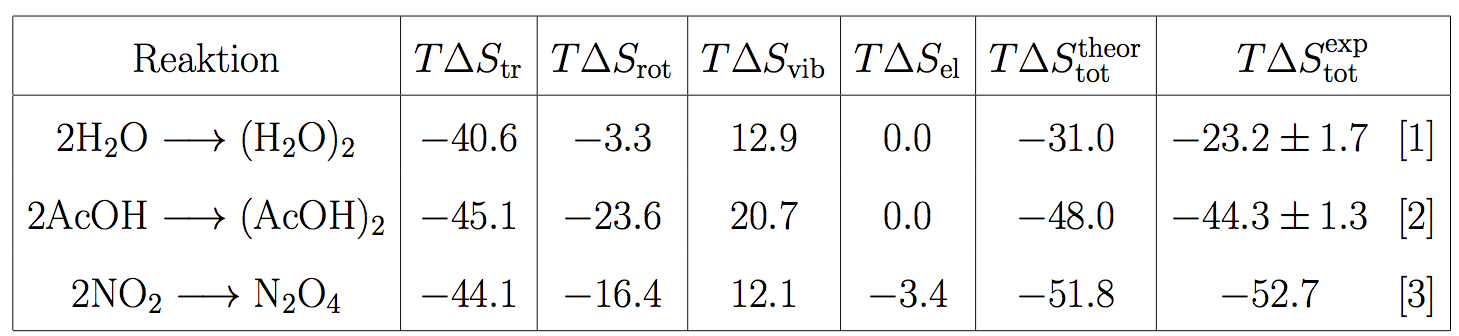
\includegraphics[width=\linewidth]{figures/zustandssummen/entropieBsp.png}
  }
\end{figure}
\vspace{-0.5cm}
\todo[inline]{Addd Kernspins (nicht in vorlesung vorgekommen) Für Proton, neutron I=1/2 (elektronen haben einen spin abner keinen Kernspin!)}
%%% Local Variables:
%%% mode: latex
%%% TeX-master: "../formularySPCS"
%%% End:

% Molekülmechanik
% ------------------------------------------------------------------------------ 
\newpage
\section{Molekühl Mechanik (MM)}
\label{sec:MM}
\begin{sectionbox}[Ziel]\nospacing
  Bisher haben wir idealisierte Systeme betrachtet \cref{defn:idealSys}.\\
  Nun wollen wir jedoch Wechselwirkungen ($\corresponds$ pot. Energie) zwischen Teilchen zulassen.
  Hierbei müssen wir zwischen der Quantemechanik und der klassischen Molekülmechanik unterscheiden.
\end{sectionbox}
\begin{sectionbox}[Problem]\nospacing
  \boxed{\text{Zustands\rd{summe}}}\tc{ulc1}{$\longrightarrow$}\boxed{\text{TD-Funktionen}} Verbindung mit der QM nur möglich, da
  wir diskrete, abzählbare Energiezustände/Eigenwerte haben $\Rightarrow$ nur lösbar für einfache Modelsysteme.\\
  \imp{Problem}: In der klassische Mechanik für molekulare Objekte (\tc{section}{MM}) sind die Energien allerdings \rd{kontinuirlich}
  und damit nicht abzählbare $\Rightarrow$ \rd{Summe} über Zustände nicht einfach berechenbar.
  \begin{align*}
    \rdb{\text{Pot. Energie}}: \Wpot=
      \begin{cases}
        \tura{\text{QM}}{\normalfont{Zustandsenergie diskret durchnum.}}: \text{Bekannt für Elementarteilchen.}\\
        \bdra{\text{MM}}{\normalfont{Zustandsenergie kontinuirlich}}: \text{leicht berechenbar.}\\
      \end{cases}
  \end{align*}
\end{sectionbox}
\begin{sectionbox}[Vorgehensweise]\nospacing
 \begin{circlelist}
     \item Finde einen analytischen Ausdruck oder eine ``vernünftige'' Approximation für die pot. Energie $\Wpot$ in eine klassischen
   mech. Beschreibung.
     \item Bestimme $\Zz$ und draus TD-Funktionen.
 \end{circlelist}
\end{sectionbox}
\begin{princpbox}
  \begin{princip}[Korrespondenzprinzip]\nospacing \leavevmode\\
    Für makroskopische Systeme muss die q.m. Beschreibung in die klassische Mechanik übergehen.
    \begin{align*}
      \lim_{\Nz\to\infty}\sum_{\nqz}\left(\text{Disk. q.m. Energie}\right)_{\nqz}&&\Longleftrightarrow&&\text{kont. Energie} 
    \end{align*}
  \end{princip}
\end{princpbox}
\subsection{Berechnung von $\Wpot=0$}
\begin{sectionbox}[\subsubsection{Translation ($\corresponds$ Teilchen im 3D Kasten)}]\nospacing
  \imp{Betrachte} System aus $\Nz$ Teilchen \imp{ohne} W.W. ($\Wpot=0$).
  \begin{align*}
    &\text{\rd{Klassisch}:}& \Hamkl&=\Ez_{\text{kin.}}=\sum_{\idxi}^{N}\frac{\pvec_{\idxi}^2}{2m}+0&&\nalign
    &\text{\rd{QM}:}& \Ham&=\Ez_{kin.}(\nqz_x^{(\idxi)},\nqz_y^{(\idxi)},\nqz_z^{(\idxi)})+0\nalign
                     &&&=\sum_{\idxi}^{N}\frac{\pi^2\hpr^2}{2mL^2}\left(\nqz_x^{(\idxi)}+\nqz_y^{(\idxi)}+\nqz_z^{(\idxi)}\right)&\forall\idxi
  \end{align*}
\end{sectionbox}
\begin{sectionbox}[$\Zz_{\text{tr.}}$ Quantenmechanisch]\nospacing
  \begin{align*}
    \Zz_{\text{tr.}}^{\text{QM}}(\Nz,\Vz,\Tz)=\frac{\zz^{\Nz}_{\text{tr}}}{\Nz!}=\prod_{\idxi}^{\Nz}\frac{1}{\Nz!}\sum_{\nqz_x^{(\idxi)},\nqz_y^{(\idxi)},\nqz_z^{(\idxi)}}\e^{-\frac{1}{\kb\Tz}\Ez_{\text{kin.}}^{\text{QM}}}
  \end{align*}
  Da L eine Makroskopische Grösse ist, kann man die Summe im Limes durch ein Integral erstezen:
  \begin{align*}
    \sum_{\nqz_x}\e^{-\betac\frac{\pi^2\hpr^2}{2mL^2}\nqz_x^2}\xrightarrow[\text{\rd{K.P.}}]{\lim\limits_{\Nz\to\infty}\nqz_x\to x}
    \int_{0}^{\infty}\e^{-\betac\frac{\pi^2\hpr^2}{2mL^2}x^2}\diff x
  \end{align*}
  \begin{align*}
     &\text{Mit }\int_{0}^{\infty}\e^{-\betac\frac{\pi^2\hpr^2}{2mL^2}x^2}\diff x\turla{=}{\cref{eq:exa2}}\frac{1}{2}\left(\frac{2 mL^2}{\betac\pi\hpr^2}\right)^{\frac{1}{2}}=\left(\frac{2 mL^2}{4\betac\pi\hpr^2}\right)^{\frac{1}{2}}
  \end{align*}
  \begin{align*}
    \zztrans=\zztrans_{x}\cdot\zztrans_{y}\cdot\zztrans_{z}=\left(\frac{2 mL^2}{4\betac\pi\hpr^2}\right)^{\frac{1}{2}+\frac{1}{2}+\frac{1}{2}}
  \end{align*}
  \begin{align}
    \boxed{\zztrans=\left(\frac{mL^2}{2\betac\pi\hpr^2}\right)^{\frac{3}{2}}=L^3\cdot\left(\frac{m}{2\betac\pi\hpr^2}\right)^{\frac{3}{2}}
    =\ul[ulc2]{V\cdot\left(\frac{m}{2\betac\pi\hpr^2}\right)^{\frac{3}{2}}}}
  \end{align}
\end{sectionbox}
\begin{sectionbox}[$\Zz_{\text{tr.}}$ KLassisch]\nospacing
  \begin{align*}
    &\text{\imp{Ansatz}: }&\e^{-\betac\Hamkl_{\text{kl.}}}=\exp\left[-\betac \left(\frac{\pimp_x^2+\pimp_y^2+\pimp_x^2}{2m}\right)\right]
  \end{align*}
  \begin{align*}
    &\zztrans_{\text{kl.}}=\mcc\underbrace{\left(\int_{-\infty}^{\infty}\diff^{3\Nz}r\right)}_{\Vz^{\Nz}}\cdot\int_{-\infty}^{\infty}\e^{-\betac \left(\frac{\pimp_x^{(i)2}+\pimp_y^{(i)2}+\pimp_z^{(i)2}}{2m}\right)}\diff^{3N}\pimp\nalign
                         &=\mcc\underbrace{\left(\int_{-\infty}^{\infty}\diff^{3\Nz}r\right)}_{\Vz^{\Nz}}\cdot\int_{-\infty}^{\infty}\exp\left[-\betac \left(\frac{\pimp_x^{2}+\pimp_y^{2}+\pimp_z^{2}}{2m}\right)\right]^{\Nz}\diff^{3N}\pimp\nalign
    &\eqs{\cref{eq:exa2}}\ul{\mcc\Vz^{\Nz}\left[2\pi m\kb\Tz\right]^{\frac{3\Nz}{2}}}
  \end{align*}
  \begin{align*}
    \ul{\zztrans_{\text{kl.}}}\eqs{\text{\rd{K.P.}}}\ul[ulc2]{\zztrans_{\text{QM}}}&&\Rightarrow&&\mcc=\frac{1}{\Nz!}\frac{1}{\hp^{3\Nz}}
  \end{align*}
  \begin{align}
    \boxed{\zztrans_{\text{kontin.}}=\frac{\Vz^{\Nz}}{\Nz!\hp^{3\Nz}}\left[2\pi m\kb\Tz\right]^{\frac{3\Nz}{2}}}
  \end{align}
\end{sectionbox}
\begin{sectionbox}[\subsubsection{Rotation ($\corresponds$ starrer Rotator)}]\nospacing
  \begin{flalign*}
    &\text{\imp{Wiederhohlung}: }&\zzrot&=\sum_{\Jqz}^{\infty}\left[(2\Jqz+1)\e^{-\betac\Ez_{\text{rot}}^{\Jqz}}\right]\nalign
    &&\Ez_{\text{rot}}^{\Jqz}&=\Jqz(\Jqz+1)\frac{\hpr^2}{2I}
  \end{flalign*}
  \imp{Annahme}: für ein makroskopisches System kann die Summe als kontinuierlich betrachtet werden.\\
  Mit Hilfe der Substitution $u:=\Jqz(\Jqz+1)=\Jqz^2+\Jqz$ folgt dann:\\
  \[\Rightarrow \frac{\diff u}{\diff \Jqz}=2\Jqz+1 \Rightarrow \diff\Jqz=\frac{\diff u}{2\Jqz+1}\]
  \begin{align*}
    \zzrot_{\text{kontin.}}&\approx\int_{0}^{\infty}(2\Jqz+1)\e^{-\frac{\betac\hpr^2\Jqz(\Jqz+1)}{2I}}\diff\Jqz=\int_{0}^{\infty}\e^{-\frac{\betac\hpr^2 u)}{2I}}\diff u\nalign
    &\eqs{\cref{eq:exa2}}\left.\left[-\frac{2I}{\betac\hpr^2}\e^{-\frac{\beta\hpr^2u}{2I}}\right]\right\rvert_{0}^{\infty}=\left(0-\left(-\frac{2I}{\betac\hpr^2}\right)\right)
  \end{align*}
  \begin{align}
    \boxed{\zzrot_{\text{kontin.}}=\frac{2I}{\betac\hpr^2}}
  \end{align}
\end{sectionbox}
  \todo[inline]{Add right tikz Picture}
% \begin{sectionbox}[Recap]\nospacing
%    \begin{tikzpicture}[node distance=1cm,
%       every node/.style={fill=sectionbox, font=\sffamily}]
%     \node (TD)[rectangle, draw]          {Jede TD-Funktion};
%     \node (Zzt)[rectangle, draw, below of=TD]          {$\Zz$};
%     \node (Zz)[rectangle, draw, below of=Zzt]          {$\Zz=\frac{\zz^N}{N!}$};
%     \node (zz)[rectangle, draw, below of=Zz]             {$\zz_{\text{m}}=\zztrans\cdot\zzrot\cdot\zzvib\cdot\zzelek$};
%     % Draw edges
%     \draw [ulc1,->] (TD) -- node {berechenbar durch} (Zzt);
%     \draw [ulc2,->] (Zzt) -- node {Zerlegung} (Zz);
%     \draw [ulc3,->] (Zz) -- node {Zerlegung} (zz);
%   \end{tikzpicture}
%\end{sectionbox}
\subsection{Berechnung von $\Wpot\neq0$}
\begin{sectionbox}\nospacing
  Für $\Wpot\neq0$ ergibt sich für die kanonische Zustands\rd{funktion}:
  \begin{align*}
    &\Zzk=\frac{1}{\Nz!\hp^{3\Nz}}\int_{-\infty}^{\infty}\int_{-\infty}^{\infty}\e^{-\betac\Ham(\vec{r}^{\Nz},\vec{p}^{\Nz})}\diff^{3\Nz}\vec{r}\diff^{3\Nz}\vec{p}
  \end{align*}
  \begin{align*}
    \Ham(\vec{r}^{\Nz},\vec{p}^{\Nz})=\Ez_{\text{kin}}(\vec{p}^{\Nz})+\Wpot(\vec{r}^{\Nz})
  \end{align*}
  \begin{flalign*}
  &\text{\imp{Mit}}&&\text{Ortskoordinaten: }&\vec{r}^{\Nz}=(r_1,\ldots,r_{\Nz})\nalign
          &&&\text{Impulskoordinaten: }& \vec{p}^{\Nz}=(p_1,\ldots,p_{\Nz})
  \end{flalign*}
  \imp{Frage}: wie kann/soll man $\Wpot(\vec{r}^{\Nz})$ wählen?\\
\end{sectionbox}
\begin{sectionbox}[\imp{Ansatz}: Zerlegung+Parameterisierung]
  \begin{numberlist}
      \item \tc{section}{Zerlegung}: Abhängig davon was man beschreiben möchte: Atome, Atomgruppen $\corresponds$ ``\rd{united Atom}''
      (z.B. Methylgruppen) = \rd{Coarse grained}.\\
      $\Rightarrow$ bestimmt durch ``Teilchen im System''
      \item \textcolor{section}{Parameterisierung}: Empirisch oder aus $\Ez_{\text{el.}}$.
  \end{numberlist}
\end{sectionbox}
\begin{sectionbox}\nospacing
  \imp{Idee}: Moleküle werden durch Stäbe, Kugeln, Scheiben,\ldots representiert.\\
  \imp{Frage}: was sind die Freiheitsgrade dieser Entitäten?
  \begin{align*}
    \Wpot=\text{Bindende W.W.}+\text{Nicht bindende W.W.}
  \end{align*}
\end{sectionbox}
\begin{sectionbox}[\subsubsection{Bindende/Intramolekulare W.W.}]\nospacing
  \begin{figure}[H]	
    \centering{\vspace{-1em}\hspace{-1cm}
      \def\svgwidth{140pt}
      \resizebox{0.8\linewidth}{!}{\input{figures/MM/intereWW.pdf_tex}}
    }
  \end{figure}
  \vspace{-1em}
  Für diese intramolekularen Freiheitsgrade ist es üblich folgende Beiträge für $\Wpot$ zu definieren:
\end{sectionbox}
\begin{sectionbox}[Streckschwingung (harm. Parabelpotential)]\nospacing
  \begin{align*}
    &\Wpot^{\text{Bond}}(\vec{r}^N)=\sum_{\idxi}\frac{1}{2}k_{\idxi}^{\text{bond}}\left[b_{\idxi}(\rvec^N)-b_{\idxi}^{\circ}\right]& \forall\idxi\in\text{Bonds}
  \end{align*}
  \begin{flalign*}
        &\text{\imp{Mit}:} &&k_{\idxi}^{\text{bond}}: &&\text{Kraftkonstante}\nalign
        &&&b_{\idxi}(\rvec^N): &&\text{Abstand von zwei Atomen zu denen eine}\nalign
        &&&&&\text{chem. Bindung postuliert wird}\nalign
        &&&b_{\idxi}^{\circ}:&&\text{Glg. Bindungslänge der $\idxi$-ten Bindung}\nalign
        &&&&&\Longleftrightarrow\text{Minimums $\Ez_{el.}$}
  \end{flalign*}
\end{sectionbox}
\begin{sectionbox}[Biegeschwingung (harm. Parabelpotential)]\nospacing
  \begin{align*}
    &\Wpot^{\text{angle}}(\vec{r}^N)=\sum_{\idxj}\frac{1}{2}k_{\idxj}^{\text{angle}}\left[\theta_{\idxj}(\rvec^N)-\theta_{\idxj}^{\circ}\right]& \forall\idxj\in\text{Angle}
  \end{align*}
  \begin{flalign*}
        &\text{\imp{Mit}:} &&k_{\idxj}^{\text{angle}}: &&\text{Kraftkonstante}\nalign
        &&&\theta_{\idxj}(\rvec^N): &&\text{Bindungswinkel von zwei Atomen zu}\nalign
        &&&&&\text{denen eine chem. Bind. postuliert wird}\nalign
        &&&\theta_{\idxj}^{\circ}:&&\text{Glg. Bindungswinkel der $\idxj$-ten Bindung}\nalign
        &&&&&\Longleftrightarrow\text{Minimums $\Ez_{el.}$}
  \end{flalign*}
\end{sectionbox}
\begin{sectionbox}[Torsion]\nospacing
  \begin{align*}
    &\Wpot^{\text{torsion}}(\vec{r}^N)=\sum_{\idxk}\frac{1}{2}k_{\idxk}^{\text{torsion}}\left\{1+\cos[m_{\idxk}\Phi_{\idxk}(\rvec)-\delta_{\idxk}]\right\}\nalign
    &\forall\idxk\in\text{Diederwinkel}\qquad\text{\imp{Mit}:}\quad \Phi_{\idxk} \text{Diederwinkel}
  \end{align*}
\end{sectionbox}
\begin{notebox}[Fitparameter]\nospacing
  \begin{align*}
    k_{\idxi}^{\text{bond}},k_{\idxi}^{\text{bond}},m_{\idxk},\delta_{\idxk}
  \end{align*}
\end{notebox}
\begin{sectionbox}[\subsubsection{Nicht bindende Wechselwirkungen}]\nospacing
  \begin{figure}[H]	
    \centering{
      \def\svgwidth{140pt}
      \resizebox{0.7\linewidth}{!}{\input{figures/MM/vdw.pdf_tex}}
    }
    \vspace{-1em}
  \end{figure}
  Für diese intermolekularen Freiheitsgrade ist es üblich folgende Beiträge für $\Wpot$ zu definieren:
\end{sectionbox}
\begin{sectionbox}[Coulomb W.W.]\nospacing
  \begin{align*}
    &\Wpot^{\text{Coulomb}}(\vec{r}^N)=\frac{1}{4\pi\epsilon_{0}\epsilon_{r}}\sum_{\substack{\text{Paare}\\\idxi<\idxj}}\frac{q_{\idxi}q_{\idxj}}{\rvec_{\idxi\idxj}}
  \end{align*}
\end{sectionbox}
\begin{sectionbox}[Van der Waals W.W. (\rd{6-12-/Lenard-Jones Potential})]\nospacing
  \begin{align*}
    &\Wpot^{\text{VdW}}(\vec{r}^N)=\sum_{\substack{\text{Paare}\\\idxi<\idxj}}4\epsilon_{\idxi\idxj}\left[\left(\frac{\sigma_{\idxi\idxj}}{\rvec{\idxi\idxj}}\right)^{12}-\left(\frac{\sigma_{\idxi\idxj}}{\rvec{\idxi\idxj}}\right)^6\right]
  \end{align*}
  \begin{flalign*}
        &\text{\imp{Mit}:} &&\epsilon_{\idxi\idxj}: &&\text{Potentialtopftiefe}\nalign
        &&&\text{$\left(\frac{\sigma_{\idxi\idxj}}{\rvec{\idxi\idxj}}\right)^{12}$}: &&\text{Abstossend \& kurzreichweitige Energie}\nalign
        &&&&&\text{$\Rightarrow$ Dominiert bei kurzer Reichweite}\nalign
        &&&\text{$\left(\frac{\sigma_{\idxi\idxj}}{\rvec{\idxi\idxj}}\right)^{6}:$}&&\text{Anziehend \& langreichweitige Energie}\nalign
        &&&&&\text{$\Rightarrow$ Dominiert bei langer Reichweite}
  \end{flalign*}
  \begin{figure}[H]
    \centering
    \begin{subfigure}{.45\columnwidth}
      \centering{
        \def\svgwidth{100pt}
        \resizebox{\linewidth}{!}{\input{figures/MM/potTopf.pdf_tex}}
      }
      \vspace{-1.5em}
      \caption{}
      \label{fig:}
    \end{subfigure}%
    \hfil
    \begin{subfigure}{.45\columnwidth}
      \centering{
        \def\svgwidth{100pt}
        \resizebox{\linewidth}{!}{\input{figures/MM/LenardJonesPotential.pdf_tex}}
      }
      \vspace{-1.5em}
      \caption{}
      \label{fig:}
    \end{subfigure}
  \end{figure}
\end{sectionbox}
\begin{sectionbox}[$R_{\text{min}}$]\nospacing
  \begin{align*}
    \vec{F}(\vec{r})&=-\nabla\Wpot(\rvec)=\frac{\diff}{\diff\vec{r}}4\epsilon\left[\rd{-}\sigma^{12}\rvec^{-12}\rd{+}\sigma^6\rvec^{-6}\right]\nalign
    &=4\epsilon\left[12\sigma^{12}\rvec^{-13}-6\sigma^6\rvec^{-7}\right]\eqs{!}0\iff \rvec^6=2\sigma^6
  \end{align*}
  \begin{align}
    R_{\text{min}}=\sqrt[6]{2}\sigma
  \end{align}
\end{sectionbox}
\begin{notebox}[Fitparameter]\nospacing
  \begin{align*}
    q_{\idxi},q_{\idxj},\epsilon_{\idxi\idxj},\sigma_{\idxi\idxj}
  \end{align*}
\end{notebox}
\begin{notebox}[Nebenbemerkung]\nospacing
  \begin{numberlist}
    \item \rd{Paarpotentialnäherung}: Mehrkörperwechselwirkung wurde vernachlässigt.
    \item Die Kräfte auf alle ``Teilchen'' des Systems erhählt man als Gradienten der pot. Energie
      \begin{align*}
        \vec{F}_{\idxi}=-\nabla_{\idxi}\Wpot(\rvec^N)=\vect{\pfrac{}{x_{\idxi}} & \pfrac{}{y_{\idxi}}& \pfrac{}{z_{\idxi}}}^{T}
      \end{align*}
  \end{numberlist}
\end{notebox}
\begin{notebox}[Kraft die von Atom j verursacht wird und auf Atom i wirkt]\nospacing
  \begin{align*}
    f_{x_{\idxi}}=&-\sum_{\substack{\idxi\\\idxi\neq\idxj}}^{N}\frac{\partial\Wpot(\rvec_{\idxi},\rvec_{\idxj})}{\partial\rvec_{\idxi\idxj}}\cdot\pfrac{r_{\idxi\idxj}}{x_{\idxi}}\nalign
    \eqs{\text{Ein Nachbaratom}}=&-\frac{\partial\Wpot(\rvec_{\idxi},\rvec_{\idxj})}{\partial\rvec_{\idxi\idxj}}\cdot\pfrac{r_{\idxi\idxj}}{x_{\idxi}}
  \end{align*}
  \begin{align*}
    \frac{\partial\Wpot(\rvec_{\idxi},\rvec_{\idxj})}{\partial\rvec_{\idxi\idxj}}=&
    4\epsilon_{\idxi\idxj}\left[-12\left(\frac{\sigma_{\idxi\idxj}}{\rvec{\idxi\idxj}}\right)^{12}+6\left(\frac{\sigma_{\idxi\idxj}}{\rvec{\idxi\idxj}}\right)^6\right]\frac{1}{\rvec_{\idxi\idxj}}
  \end{align*}
  \begin{align*}
  &\pfrac{r_{\idxi\idxj}}{x_{\idxi}}=\frac{\partial}{\partial x_{\idxi}}\left[(x_{\idxi}-x_{\idxj})^2+(y_{\idxi}-y_{\idxj})^2+(z_{\idxi}-z_{\idxj})^2\right]^{\frac{1}{2}}\nalign
  &=\frac{1}{2}\left[(x_{\idxi}-x_{\idxj})^2+(y_{\idxi}-y_{\idxj})^2+(z_{\idxi}-z_{\idxj})^2\right]^{-\frac{1}{2}}2(x_{\idxi}-x_{\idxj})\nalign
    &=\frac{x_{\idxi\idxj}}{\rvec_{\idxi\idxj}}
  \end{align*}
  \begin{align*}
    f_{x_{\idxi}}=-4\epsilon_{\idxi\idxj}\left[-12\left(\frac{\sigma_{\idxi\idxj}}{\rvec{\idxi\idxj}}\right)^{12}+6\left(\frac{\sigma_{\idxi\idxj}}{\rvec{\idxi\idxj}}\right)^6\right]\frac{x_{\idxi\idxj}}{\rvec_{\idxi\idxj}^2}
  \end{align*}
\end{notebox}
\begin{sectionbox}[Damit ergibt sich]\nospacing
  \begin{align}
    \Wpot=\Wpot^{\text{bond}}+\Wpot^{\text{angle}}+\Wpot^{\text{torision}}+\Wpot^{\text{Coul.}}+\Wpot^{\text{VdW}}
  \end{align}
\end{sectionbox}
\begin{sectionbox}[\subsection{Berechnung der Zustandsfunktion}]\nospacing
  Wir haben nun einen analytischen ausdruck für $\Wpot$ gefunden und können nun die komplette Zustands\rd{funktion} berechnen:
  \begin{align*}
    &\Zzk=\frac{1}{\Nz!\hp^{3\Nz}}\iint_{-\infty}^{\infty}\e^{-\betac\Ham(\vec{r}^{\Nz},\vec{p}^{\Nz})}\diff^{3\Nz}\vec{r}\diff^{3\Nz}\vec{p}
  \end{align*}
  \begin{align*}
    \Ham(\vec{r}^{\Nz},\vec{p}^{\Nz})=\sum_{\idxi=1}^{N}\frac{\prescript{N}{}{\pvec}_{\idxi}^2}{2m_{\idxi}}+\Wpot(\vec{r}^{\Nz})
  \end{align*}
  \begin{alignat*}{3}
    \Zzk&\eqs{\Wpot\neq0}&&\mcc[\frac{1}{\hp^{3N}N!}]\int_{-\infty}^{\infty}\exp\left(-\betac\sum_{\idxi=1}^{N}\frac{\prescript{N}{}{\pvec}_{\idxi}^2}{2m_{\idxi}}\right)\diff^{3N}\pimp\nalign
    &&&\cdot\int_{-\infty}^{\infty}\e^{-\betac\Wpot(\rvec^N)}\diff^{3\Nz}r
  \end{alignat*}
  \begin{alignat*}{2}
    &\eqs{\cref{eq:eIntegral}}&\mcc[\frac{1}{\hp^{3N}N!}]\prod_{\idxi}^N \left(2\pi\m_{\idxi}\kb\Tz\right)^{\frac{3}{2}}\cdot\int\limits_{-\infty}^{\infty}\e^{-\betac\Wpot(\rvec^N)}\diff^{3\Nz}r
  \end{alignat*}
  Mit der Annahnme gleicher Massen: $m_{\idxi}=m\quad\forall\idxi$ folgt:
  \begin{align*}
        &\eqs{\hphantom{\cref{eq:eIntegral}}}\underbrace{\frac{1}{N!}\left(2\pi\hp^{-2}\m\kb\Tz\right)^{\frac{3N}{2}}}_{\equiv\tc{ulc1}{f}}\cdot\underbrace{\int\limits_{-\infty}^{\infty}\e^{-\betac\Wpot(\rvec^N)}\diff^{3\Nz}r}_{\equiv\Qzk}
  \end{align*}
  Damit ergibt sich für Observablen $\Omega$:
  \todo[inline]{Warum?}
  \begin{alignat*}{2}
    &\obs{\Omega}_{\Nz,\Vz,\Tz}&&=\frac{\iint_{-\infty}^{\infty}\Omega(\rvec^N)\e^{-\betac\Ham(\vec{r}^{\Nz},\vec{p}^{\Nz})}\diff^{3\Nz}\vec{r}\diff^{3\Nz}\vec{p}}{\Zzk}\nalign
    &&&=\frac{\int_{-\infty}^{\infty}\Omega(\rvec^N)\cdot\e^{-\betac\Wpot(\rvec^N)}\diff^{3\Nz}r\cdot\cancel{\tc{ulc1}{f}(\pvec^N)}}{\int_{-\infty}^{\infty}\e^{-\betac\Wpot(\rvec^N)}\diff^{3\Nz}r\cdot\cancel{\tc{ulc1}{f}(\pvec^N)}}\nalign
    &&&\equiv\int_{-\infty}^{\infty}\Omega(\rvec^N)\pbr(\rvec^N)\diff^{3\Nz}r
  \end{alignat*}
\end{sectionbox}
\begin{defnbox}\nospacing
  \begin{defn}[Konfigurationszustandssumme/integral]
    \begin{align}
      \Qzk=\int\limits_{-\infty}^{\infty}\e^{-\betac\Wpot(\rvec^N)}\diff^{3\Nz}r
    \end{align}
    \todo[inline]{Haben wir dann nicht ein Doppelintegral über $\Qzk$ wenn wir in $\pbr$ einsetzen?}
    \begin{flalign}
      &\text{\imp{Mit}}:&&\pbr(\rvec^N)=\frac{\e^{-\betac\Wpot(\rvec^N)}}{\Qzk}&\nalign
      &\text{und}:&&\obs{\Omega}_{\Nz,\Vz,\Tz}=\int\limits_{-\infty}^{\infty}\Omega(\rvec^N)\pbr(\rvec^N)\diff^{3\Nz}r
    \end{flalign}
  \end{defn}
\end{defnbox}
\begin{sectionbox}[\subsubsection{Berechnung von $\Qzk$}]\nospacing
  \imp{Problem}: Analytische Lösung i.d.R. nicht möglich.\\
  $\Rightarrow$ Nummerische Integration.\\
  \imp{Problem}: Bei 10 Gitterpunkten pro Freiheitsgrad  ergeben sich $10^{3\idxN}$ Punkte an denen der Integrand zu berechnen ist.
  Mit $\idxN=10^{24}$ Teilchen schon nicht mehr möglich.
\end{sectionbox}

	\vfill\columnbreak
\subsection{Stochastische Lösungen/Samplingsmethoden}
\begin{sectionbox}[\subsubsection{Random Sampeling}]\nospacing
  \begin{align*}
    \Qzk&=\int_{\rvec_{\mca}}^{\rvec_{\mcb}}\e^{-\betac\Wpot(\rvec^N)}\diff\rvec^N\qquad \rvec=(r_x,r_y,r_z)\nalign
    &=\obs{\e^{-\betac\Wpot(\rvec^N)}}\underbrace{\prod_{\idxi}^{3N}(\rvec_{\idxi,\mcb}-\rvec_{\idxi,\mca})}_{\text{Volumen der Domain}}\nalign
    &\approx\frac{1}{n_{\pb}}\sum_{\idxj=1}^{n_{\pb}}\prod_{\idxi=1}^{3N}(\rvec_{\idxi,\mcb}-\rvec_{\idxi,\mca})\cdot\e^{-\betac\Wpot(\rvec_{\idxi}^N)}
  \end{align*}
  \begin{wrapfigure}{l}{0.4\linewidth}	
    \centering{
      \vspace{-1em}
      \inkscape[80pt]{figures/MM/randomnSampeling.pdf_tex}
    }
  \end{wrapfigure}
  \begin{flalign*}
    &\hspace{-2em}\approx\frac{1}{n_{\pb}}\sum_{\idxj=1}^{n_{\pb}}\prod_{\idxi=1}^{3N}(\rvec_{\idxi,\mcb}-\rvec_{\idxi,\mca})\cdot\e^{-\betac\Wpot(\rvec_{\idxi}^N)}
  \end{flalign*}
  \begin{flalign*}
    &n_{\pb}:&& \text{Anzahl der gewählten}&\nalign
    &&&\text{Konfigurationen}&
  \end{flalign*}
\end{sectionbox}
\todo[inline]{Check index of $\Wpot: \idxi$ oder $\idxj$ und wie kommt man auf die Formel?}
\begin{notebox}[Note]
  \begin{numberlist}
      \item Die $n_{\pb}$ Konfigurationen im Intervall $[\rvec_{\mca}^N,\rvec_{\mcb}^N]$ werden zufäfllig gewählt.
      \item Alle $\rvec_{\idxi}^N$ haben diesielbe Wahrscheinlichkeit.
      \item Sehr ineffizient, da $n_{\pb}$ sehr gross sein muss.
  \end{numberlist}
\end{notebox}
\begin{sectionbox}[\subsubsection{Importance Sampeling}]\nospacing
  \imp{Idee}: beprobe/sample nicht zufällig sondern wähle die $\{\rvec_{\idxi}^N\}$ anhand einer Wahrscheinlichkeitsverteilung, so dass der \rd{Boltzmann Faktor} $\e^{-\betac\Wpot(\rvec_{\idxi}^N)}$ gross wird.
\end{sectionbox}
\begin{sectionbox}[\subsubsection{Metropolis-Monte-Carlo Algorithm}\normalfont{(Variante des Importance Sampling})]\nospacing
  \imp{Grundidee}:
  \begin{circlelist}
    \item Zufällige Auswahl an Konfigurationen $r_{\idxi}^N$.
    \item Übernehme oder verwerfe die Konfigurationen $r_{\idxi}^N$ auf Grund der Boltzmann Verteilung.
    \item Berechne $\obs{\Omega}_{\Nz,\Vz,\Tz}$ aus den akzeptierten $r_{\idxi}^N$.
  \end{circlelist}
\end{sectionbox}
\begin{sectionbox}[Konkrete Implementation]\nospacing
  \imp{Voraussetzung}: grosse Anzahl an Schritten.
  \begin{circlelist}
    \item Generiere eine neue Konfiguration: $\rvec_{\idxi+1}^N=\rvec_{\idxi}^N+\Delta\rvec^N$\\
     $\Delta\rvec^N$: gibt verschiedene Möglichkeiten dies zu wählen.
    \item Berechne die Änderung der Energie\\\ctr{$\Delta\Wpot=W(\rvec_{\idxi+1}^N)-W(\rvec_{\idxi}^N)$}
    \item Akzeptiere $\rvec_{\idxi+1}^N$ auf Grund der Boltzmann-Verteilung falls:
    \begin{numberlist}
        \item $\Delta\Wpot\leq0$ (pot. Energie nimmt ab)\hfil\imp{oder}
        \item $\Delta\Wpot>0$\hfil \imp{und} \hfil$\e^{-\frac{\Delta\Wpot}{\kb\Tz}}>\epsilon$\\
          \imp{Mit}\hfil der Zufallszahl: $\epsilon\in[0,1]$
    \end{numberlist}
    ansonsten verwerfe $\rvec_{\idxi+1}^N$.
    \item Repeat.
  \end{circlelist}
  \begin{figure}[H]	
    \centering{
      \def\svgwidth{160pt}
      \resizebox{0.7\linewidth}{!}{\input{figures/MM/MMC.pdf_tex}}
    }
  \end{figure}
\end{sectionbox}
\begin{notebox}[Parameter des MC-Algorithmus]
  \begin{numberlist}
      \item Anzahl der Schritte.
      \item $\Delta\rvec^n$.
  \end{numberlist}
\end{notebox}
\begin{notebox}[Effizienz der Beprobung]\nospacing
  \begin{numberlist}
      \item Schrittgrösse $\Delta\rvec$ sehr/zu gross $\Rightarrow$ $\Delta\Wpot$ gross:
      \begin{align*}
        \Rightarrow \e^{-\frac{\Delta\Wpot}{\kb\Tz}}\approx0&&\Rightarrow&&\e^{-\frac{\Delta\Wpot}{\kb\Tz}}\stackrel{\text{i.d.R.}}{\ngtr}\epsilon
      \end{align*}
      $\Rightarrow$ verwerfen für $\Delta\Wpot>0$ so gut wie immer.
        \item Schrittgrösse $\Delta\rvec$ zu klein:\\
      Limitierte Beprobung, suchen nur kleinen Teil des Raumes ab.
  \end{numberlist}
  $\Rightarrow$ Effizienz hängt von der Balance zwischen der Schrittgröse und der Akkzeptanz/Verwerfungsrate ab.
\end{notebox}
\begin{notebox}[Nebenbemerkung]
  Wir benutzen hier die Boltzmann-Gewichtung und beproben das kanonische Ensemble.\\
  $\Rightarrow$ falls man einen anderes Ensemble beproben will muss man sich überlegen wie man dies am besten macht.
\end{notebox}
\begin{sectionbox}[\subsubsection{Replica Exchange Simulation/Parallel tempering}]\nospacing
  \begin{flalign*}
    &\imp{\text{Recall}:}&\nalign
    &&\hspace{-1cm}\Zz_{\text{klassisch}}(\Nz,\Vz,\Tz)\sim\Qzk=\int_{-\infty}^{\infty}\e^{-\betac\Wpot(\rvec^N)}\diff^{3\Nz}r
  \end{flalign*}
  \imp{Problem}: MD-Simulationen erfordern häufig \rd{ergodisches} Peproben von (Energie)konfigurationsräume mit vielen Minima und Barrieren
  zwischen Minima. Diese sind bei Raumtemperatur nur schwer zu durchequeren $\Rightarrow$ Die Ergebnisse der MD-Simulationen sind oft durch die Wahl der Startbedingunen (inital conditions) beschränkt.\\
  \imp{Frage}: können wir dieses Problem der limitierten Beprobung beheben?\\
  \imp{Idee}: Es geht uns draum das Integral zu sampeln, wie wir auf das Ergebnis kommen/die $\rvec_{\idxi}^N$ wählen ist nicht so relevant.\\
  $\Rightarrow$ simuliere simultan viele unabhängige Kopien von Ensembles/Systemen e.g. $\idxk$ und $\idxk'$ und vertausche die entsprechenden
  Konfigurationen $\rvec_{\idxk}^N$ mit $\rvec_{\idxk'}^N$ von Zeit zu Zeit.
  Typischerweise werden die Kopien so gewählt, dass das eine Extrem der Kopien das System ist das wir beproben wollen und das andere Extrem
  ein System ist in dem die Barrieren leichter überwunden werden können.\\
  Kopien können dabei simuliert werden für:
  \begin{numberlist}
    \item Verschiedene Thermodynamische Randbedingungen (z.B. Temperatur).
    \item Verschiedene Hamilton-Funktionen (z.B. verschiedene Kraftfelder).
  \end{numberlist}
\end{sectionbox}
\begin{sectionbox}[Vorgehen]\nospacing
  In bestimmten Intervallen werden nun die Konfigurationen/Koordinaten $\rvec_{\idxk}^N$ und $\rvec_{\idxk'}^N$ zweier Kopien $\idxk$ und
  $\idxk'$ mit einer Wahrscheinlichkeit $\pb$ ausgetauscht.
  \begin{align}
    \pb(\idxk\leftrightarrow\idxk')=\min\left(1,\e^{\mcc[\Delta]}\right):=\begin{cases}
        1 &\text{für } \mcc[\Delta]\leq0\\
        \e^{\mcc[\Delta]} &\text{für } \mcc[\Delta]>0
      \end{cases}
  \end{align}
  \begin{flalign*}
    &\rd{\text{Temperatur}}:&\mcc[\Delta]_{\Tz}\equiv\left[\frac{1}{\kb\Tz_{\idxk}}-\frac{1}{\kb\Tz_{\idxk'}}\right]\left[\Hamkl(\rvec_{\idxk'}^N)-\Hamkl(\rvec_{\idxk}^N)\right]
  \end{flalign*}
  \begin{flalign*}
    &\rd{\text{Verschiedene Kraftfelder}}:\mcc[\Delta]_{\Wpot}\equiv\nalign
    &\frac{\left[\Hamkl(\rvec_{\idxk'}^N,\Wpot_{\idxk})-\Hamkl(\rvec_{\idxk}^N,\Wpot_{\idxk})\right]-\left[\Hamkl(\rvec_{\idxk'}^N,\Wpot_{\idxk'})-\Hamkl(\rvec_{\idxk}^N,\Wpot_{\idxk'})\right]}{\kb\Tz}
  \end{flalign*}
\end{sectionbox}
%%% Local Variables:
%%% mode: latex
%%% TeX-master: "../formularySPCS"
%%% End:
% Molekül Dynamik
% ------------------------------------------------------------------------------ 
% ======================================================================
\newpage
\section{Molekül Dynamik (MD)}
\label{sec:MD}
\begin{sectionbox}\nospacing
  \imp{Idee}: Beprobung des Konfigurationsraumes durch Verflogung
  einer Trajektorie, unter Verwendung einer adequaten
  Bewegungsgleichung.\\
  \imp{In anderen Worten}: Beprobung durch explizite zeitliche Propagation des Systems per Newton Bewegungsgleichung.
\end{sectionbox}
\begin{notebox}[MD-Simulation und andere Ensemble]
  Die Lösung der Bewegungsgleichung konserviert die Energie $\Rightarrow$ \rd{Mikrokanonisches Ensemble}!\\
  \imp{Frage}: wie kommen wir zurück zum \rd{kanonische Ensemble}?\\
  Stochastische Beprobung unter Verwendung des Boltzmann-Gewichts $\Longleftrightarrow$ MMC.
\end{notebox}
\begin{sectionbox}[Zu lösen]\nospacing
  \begin{align}
    m_{\idxi}\frac{\diff^2\rveci}{\diff t^2}=-\nabla_{\idxi}\Wpot\left(\rvec^N(t)\right)&&
           \nabla_{\idxi}=\vect{\frac{\partial}{\partial x_{\idxi}} \\ \frac{\partial}{\partial y_{\idxi}} \\ \frac{\partial}{\partial z_{\idxi}}}\label{eq:eqOfMotion}
  \end{align}
  Diese Dgl 2. Ordnung kann zu zwei Dgls 1. Ordnung reduziert werden:
  \begin{align}
    &\dot{\rvec}(t)=\vvec(t)&&\text{und}&&\dot{\vvec}(t)=\frac{F(\rvec(t))}{m}\label{eq:eqOfMotion2}
  \end{align}
\end{sectionbox}
\begin{notebox}[Problem]
  Analytische Lösung auf Grund der Form des Kraftfeldes $\Wpot$ nicht möglich $\Rightarrow$ Diskretisierung.
\end{notebox}
\subsection{Leap Frog Algorithmus}
\label{subsec:LeapFrogAlgorithmus}
\begin{sectionbox}\nospacing
  \begin{numberlist}
    \item Gitter von äquidistanten Punkten $\left\{t_{\idxn}\right\}_{\idxn=1}^{M}$.
    \item Maschenweite (Stepsize): $\Delta \frac{t}{2}$.
    \item $\Delta t$ wird in abhängig von der Dynamik des Systems gewählt, damit die komplette Dynamik erfasst wird. $\Delta t$ typischerweise $\approx10\femto\second$.
  \end{numberlist}
  \imp{Notation}:\hfil$\rvec^N\hfil\Longleftrightarrow\hfil\rveci\quad\forall\idxi$\\
  \imp{Gegeben}: $\rveci(\tnp)$ zum Zeitpunkt $\tnp\eqs{\text{e.g.}}t_0$.\\
  \imp{Gesucht}: $\rveci(\tnp+\Delta t)\quad\forall\idxi\Rightarrow$ Taylor Entwickelung.
  \begin{alignat*}{3}
    &\rveci(\tnp+\Delta t)&&=\nalign
                            &&&\rveci(\tnp)+\Delta t\left.\difrac{\rveci}{t}\right\rvert_{\tnp}+\frac{1}{2}\Delta t^2\left.\frac{\diff^2\rveci}{\diff t^2}\right\rvert_{\tnp}+\bigO{\Delta t^3}
  \end{alignat*}
  \imp{Problem}: $\frac{\diff^2\rveci}{\diff t^2}$ ist nicht explizit bekannt.\\
  \imp{Idee}: wähle den Zeitschritt geschickt um $\frac{\diff^2\rveci}{\diff t^2}$ zu eliminieren.
  \begin{alignat}{2}
    &\rveci\left(\tnp+\frac{\Delta t}{2}\right)=\label{eq:lf1}\nalign
                            &\quad=\rveci(\tnp)+\frac{\Delta t}{2}\left.\difrac{\rveci}{t}\right\rvert_{\tnp}+\frac{1}{2}\left(\frac{\Delta t}{2}\right)^2\left.\frac{\diff^2\rveci}{\diff t^2}\right\rvert_{\tnp}+\bigO{\Delta t^3}\nonumber\nalign
    &\rveci\left(\tnp-\frac{\Delta t}{2}\right)=\label{eq:lf2}\nalign
                            &\quad=\rveci(\tnp)-\frac{\Delta t}{2}\left.\difrac{\rveci}{t}\right\rvert_{\tnp}+\frac{1}{2}\left(\frac{\Delta t}{2}\right)^2\left.\frac{\diff^2\rveci}{\diff t^2}\right\rvert_{\tnp}+\bigO{\Delta t^3}\nonumber
  \end{alignat}
  \begin{alignat*}{2}
    &\cref{eq:lf1}-\cref{eq:lf2}=\cancel{2}\cdot\frac{\Delta t}{\cancel{2}}\uldotted{\left.\difrac{\rveci}{t}\right\rvert_{\tnp}}+\bigO{2\cdot\Delta t^3}\nalign
    &\Rightarrow\rveci\left(\tnp+\frac{\Delta t}{2}\right)=\rveci\left(\tnp-\frac{\Delta t}{2}\right)+\Delta t\cdot\uldotted{\vveci(\tnp)}+\bigO{\Delta t^3}
  \end{alignat*}
  \imp{Kosmetik}: um dies nun wieder zu ganzen Zeitschritten umzuwandeln setzen wir einfach: $\tnp=\tn+\frac{\Delta t}{2}$:
    \begin{align*}
      &\Rightarrow\rveci\left(\tn+\Delta t\right)=\rveci\left(\tn\right)+\Delta t\cdot\vveci\left(\tn+\frac{\Delta t}{2}\right)+\bigO{\Delta t^3}
    \end{align*}
    \imp{Problem}: $\vveci\left(\tn+\frac{\Delta t}{2}\right)$ ist auch unbekannt $\Rightarrow$ Taylor entwickelung.
  \begin{alignat}{2}
    &\vveci\left(\tn+\frac{\Delta t}{2}\right)=\label{eq:lf3}\nalign
                            &\quad=\vveci(\tn)+\frac{\Delta t}{2}\left.\difrac{\vveci}{t}\right\rvert_{\tn}+\frac{1}{2}\left(\frac{\Delta t}{2}\right)^2\left.\frac{\diff^2\vveci}{\diff t^2}\right\rvert_{\tn}+\bigO{\Delta t^3}\nonumber\nalign
    &\vveci\left(\tn-\frac{\Delta t}{2}\right)=\label{eq:lf4}\nalign &\quad=\vveci(\tn)-\frac{\Delta t}{2}\left.\difrac{\vveci}{t}\right\rvert_{\tn}+\frac{1}{2}\left(\frac{\Delta t}{2}\right)^2\left.\frac{\diff^2\vveci}{\diff t^2}\right\rvert_{\tn}+\bigO{\Delta t^3}\nonumber
  \end{alignat}
  \begin{alignat*}{2}
    \cref{eq:lf3}-\cref{eq:lf4}&=\cancel{2}\cdot\frac{\Delta t}{\cancel{2}}\uldotted[ulc2]{\left.\difrac{\vveci}{t}\right\rvert_{\tn}}+\bigO{2\cdot\Delta t^3}\nalign
    \Rightarrow\vveci\left(\tn+\frac{\Delta t}{2}\right)&=\vveci\left(\tn-\frac{\Delta t}{2}\right)+\uldotted[ulc2]{\aveci(\tn)}\Delta t+\bigO{\Delta t^3}\nalign
  \end{alignat*}
  Mit Newton $F_{\idxi}=m_{\idxi}\aveci$ und $-\nabla_{\idxi}\Wpot\left(\rvec^N(t)\right)$ folgt:
\end{sectionbox}
\begin{defnbox}\nospacing
  \begin{defn}[Leap-Frog Algorithm]
    \begin{alignat}{2}
      \vveci\left(\tn+\frac{\Delta t}{2}\right)&=\vveci\left(\tn-\frac{\Delta t}{2}\right)-\frac{\Delta t}{m_{\idxi}}\nabla_{\idxi}\Wpot\left(\rvec^N(\tn)\right)\nonumber\nalign
      \rveci\left(\tn+\Delta t\right)&=\rveci\left(\tn\right)+\Delta t\cdot\vveci\left(\tn+\frac{\Delta t}{2}\right)\nalign
                                                 \text{\imp{Error}}&=\bigO{\Delta t^3}\nonumber
    \end{alignat}
    \begin{figure}[H]	
      \centering{
        \vspace{-1em}
        \def\svgwidth{180pt}
        \resizebox{0.8\linewidth}{!}{\input{figures/MD/leapFrog.pdf_tex}}
      }
    \end{figure}
  \end{defn}
\end{defnbox}
\begin{notebox}[$\rveci\left(\tn+\Delta t\right)$ wird berechnet aus:]
  \begin{numberlist}
      \item Ort zum Zeitpunkt $\tn$.
      \item Geschwindikeit zu den Zeiten: $\tn-\frac{\Delta t}{2}$ und $\tn+\frac{\Delta t}{2}$.
      \item Der Kraft zum Zeitpunkt $\tn$.
  \end{numberlist}
\end{notebox}
\begin{notebox}[Initalisierung des Algorithmus]
  \begin{circlelist}
      \item Lege Position aller ``Teilchen'' vernüftig fest.\\
    Leicht machbar: chem. vernüftige Struktur.
      \item Bestimme Anfangsgeschwindikeiten anand von stat. Überlegungen:
    \begin{numberlist}
        \item Maxwell-Boltzmann Geschwindigkeitsverteilung \imp{oder}
        \item Mittler gleichverteilte Geschwindigkeitsverteilung.
    \end{numberlist}
  \end{circlelist}
\end{notebox}
\subsection*{Geschwindkeitsverteilungen}
\todo[inline]{Add Parts}
\begin{sectionbox}[\subsubsection{Maxwell-Boltzmann-Geschwindikeitsverteilung}]\nospacing
  
\end{sectionbox}
\begin{sectionbox}[\subsubsection{Gleichverteilung}]\nospacing
  
\end{sectionbox}
\begin{sectionbox}[\subsection{Verlet-Algorithmus}]\nospacing
   Entwickle um $\rvec(t\pm\Delta t)$:
  \imp{Nebenbemerkung}: indices der einfachheithalber weggelassen.
    \begin{alignat}{3}
    &\ul{\rvec(t+\Delta t)}=&&\rvec(t)+\Delta t\left.\difrac{\rvec}{t}\right\rvert_{t}+\frac{1}{2}\Delta t^2\left.\frac{\diff^2\rvec}{\diff t^2}\right\rvert_{t}+&&\nonumber\nalign
    &&&+\frac{1}{6}\Delta t^3\left.\frac{\diff^3\rvec}{\diff t^3}\right\rvert_{t}+\bigO{\Delta t^4}\label{eq:verlet1}&&\nalign
    &\uldotted{\rvec(t-\Delta t)}=&&\rvec(t)-\Delta t\left.\difrac{\rvec}{t}\right\rvert_{t}+\frac{1}{2}\Delta t^2\left.\frac{\diff^2\rvec}{\diff t^2}\right\rvert_{t}-&&\nonumber\nalign
    &&&-\frac{1}{6}\Delta t^3\left.\frac{\diff^3\rvec}{\diff t^3}\right\rvert_{t}+\bigO{\Delta t^4}&&\label{eq:verlet2}
  \end{alignat}
  Mit \cref{eq:verlet1}-\cref{eq:verlet2} folgt:
  \begin{alignat*}{2}
    &\rvec(t+\Delta t)=2\rvec(t)+\rvec(t-\Delta t)+\avec(t)\Delta t^2+\bigO{\Delta t^4}
  \end{alignat*}
\end{sectionbox}
  \begin{notebox}[Problem]
    \begin{numberlist}
        \item $\avec(t)$ unbekannt $\Rightarrow$ benutze \rd{Differenzquotient}.
        \item Bei MD-simulationen wird die Energie nicht automatische erhalten $\Rightarrow$ sollten darauf achten das
      $\Ez=\Ez_{\text{kin.}}+\Wpot=$konstant.\\
      \imp{Problem}: $\vvec$ in $\Ez_{kin.}=\frac{1}{2}m\vvec^2$ ist hier nicht bekannt, aber mit Taylor folgt auch:
        \begin{align*}
          \vvec(t)=\frac{\ul{\rvec(t+\Delta t)}-\uldotted{\rvec(t-\Delta t)}}{2\Delta t}+\rd{\bigO{\Delta t^2}}
        \end{align*}
        \imp{Problem}: Fehler nicht mehr $\bigO{\Delta t^4}$ sondern $\bigO{\Delta t^2}$.  
    \end{numberlist}
  \end{notebox}
\begin{defnbox}\nospacing
  \begin{defn}[Störmer/Verlet-Algorithmus]
    \begin{align}
      \rvec(t+\Delta t)&=2\rvec(t)+\rvec(t-\Delta t)+\mcc[\avec(t)]\Delta t^2+\bigO{\Delta t^4}\nalign
      \mcc[\avec(t)]&\bdrla{=}{\normalfont{\rd{3-Punkte-Zentraldifferenzenquotient}}}\frac{\diff^2\rvec(t)}{\diff t^2}=\frac{\rvec(t+\Delta t)-2\rvec(t)+\rvec(t-\Delta t)}{\Delta t^2}\nonumber\nalign
                                                 \text{\imp{Error}}&=\bigO{\Delta t^4}\nonumber
    \end{align}
    \begin{align}
      &\Ez=K+\Wpot\quad\text{mit}\quad\vvec(t)=\frac{\rvec(t+\Delta t)-\rvec(t-\Delta t)}{2\Delta t}+\bigO{\Delta t^2}
    \end{align}
  \end{defn}
\end{defnbox}
\begin{proofbox}\nospacing
    \begin{proof}
      \begin{align*}
        \mcc[\avec(t)]=\frac{\diff^2\rvec(t)}{\diff t^2}&=\frac{\frac{\rvec(t+\Delta t)-\rvec(t)}{\Delta t}-\frac{\rvec(t)-\rvec(t-\Delta t)}{\Delta t}}{\Delta t}\nalign
                                                          &=\frac{\rvec(t+\Delta t)-2\rvec(t)+\rvec(t-\Delta t)}{\Delta t^2}
      \end{align*}
    \end{proof}
\end{proofbox}
\begin{notebox}[Vorteil]
  \begin{numberlist}
      \item Kommt ohne halbe Zeitschritte aus.
      \item Kommt ohne Geschwindigkeit aus.
  \end{numberlist}
\end{notebox}
\begin{sectionbox}[\subsection{Velocity-Verlet-Algorithmus}]\nospacing
  \begin{flalign*}
    &\text{Recall \cref{eq:eqOfMotion2}:} &\mca[\dot{\rvec}](t)=\vvec(t)&&\text{und}&&\mcb[\dot{\vvec}](t)=\frac{F(\rvec(t))}{m}
  \end{flalign*}
  Mit Taylor folgt dann wieder:
  \begin{align*}
    \mca[\rvec(t+\Delta t)]=&\rvec(t)+\Delta t\left.\difrac{\rvec}{t}\right\rvert_{t}+\frac{1}{2}\Delta t^2\left.\frac{\diff^2\rvec}{\diff t^2}\right\rvert_{t}+\bigO{\Delta t^3}
  \end{align*}
  Für $\frac{\diff^2\rvec}{\diff t^2}$ benutzen wir $\avec(t)=-\frac{\nabla\Wpot(t)}{m}$ und für $\difrac{\rvec}{t}=\vvec(t)$.
  Für $\mcb[\dot{\vvec}](t)$ folgt dann analog:
  \begin{align*}
    \mcb[\vvec(t+\Delta t)]=&\vvec(t)+\Delta t\left.\difrac{\vvec}{t}\right\rvert_{t}+\ul[ulc2]{\frac{1}{2}\Delta t^2\left.\mcc[\frac{\diff^2\vvec}{\diff t^2}]\right\rvert_{t}}+\bigO{\Delta t^3}
  \end{align*}
  Für $\difrac{\vvec}{t}$ benutzen wir wieder
  $\avec(t)=-\frac{\nabla\Wpot(t)}{m}$ und für $\mcc[\frac{\diff\avec}{\diff t}]=\frac{\diff^2\vvec}{\diff t^2}$ benutzen wir wieder Taylor:
  \begin{align}
   \avec(t+\Delta t)=&\avec(t)+\Delta t\mcc[\left.\difrac{\avec}{t}\right\rvert_{t}]+\bigO{\Delta t^2}\label{eq:velocityv1}
  \end{align}
  Es ist ausreichen bis zur Ordnung $\bigO{\Delta t^2}$ zu entwickeln da wir einen Ausdruck für
  $\frac{\Delta t^2}{2}\left.\mcc[\frac{\diff^2\vvec}{\diff t^2}]\right\rvert_{t}$ suchen: \cref{eq:velocityv1}$\cdot\frac{\Delta t}{2}$:
  \begin{align*}
    &\ul[ulc2]{\frac{\Delta t^2}{2} \left.\difrac{\avec}{t}\right\rvert_{t}}=\frac{\Delta t}{2}\left(\mcc[\avec(t+\Delta t)]-\avec(t)\right)+\bigO{\Delta t^{\rd{3}}}
  \end{align*}
\end{sectionbox}
\begin{defnbox}\nospacing
  \begin{defn}[Velocity-Verlet]
    \begin{align}
      &\circledItem{1}& \rvec(t+\Delta t)=&\rvec(t)+\Delta t\left.\difrac{\rvec}{t}\right\rvert_{t}+\frac{1}{2}\Delta t^2\left.\frac{\diff^2\rvec}{\diff t^2}\right\rvert_{t}+\bigO{\Delta t^3}\nonumber\nalign
      &\circledItem{2}& \avec(t+\Delta t)&=-\frac{\nabla\Wpot(t+\Delta t)}{m}\nonumber\nalign
      &\circledItem{3}& \vvec(t+\Delta t)&=\vvec(t)+\frac{\avec(t)+\avec(t+\Delta t)}{2}\Delta t\nonumber\nalign
                                                 &&\text{\imp{Error}}&=\bigO{\Delta t^3}
    \end{align}
  \end{defn}
\end{defnbox}
\begin{notebox}[Nebenbemerkungen]
  \begin{numberlist}
      \item Für den Velocity-Verlet Algorithmus müssen wir zur Initalisierung auch einmal $\vvec(t)$ bestimmen/setzen.
      \item Alle drei Algorithmen sind Zeitinvariant, sind also symetrisch bezüglich der Zeit.
  \end{numberlist}
\end{notebox}
%%% Local Variables:
%%% mode: latex
%%% TeX-master: "../formularySPCS"
%%% End:

% Stochastische MD
% ------------------------------------------------------------------------------ 
\newpage
\section{Stochastische Molekül Dynamik}
\subsection{SMD/Langerin-Dynamik}
\label{subsec:SMD/LangerinDynamik}
\begin{sectionbox}[Einführung]\nospacing
  Ist eine stochastische Variante der MD zur Beschreibung komplexer Systeme.\\
  \imp{Aufgabenstellung}: simulation von ``Teilchen'' die einer schneller fluktuierenden Umgebung ausgestzt sind Bsp.:
  \begin{numberlist}
    \item Fettblasen in Suppe.
    \item Polymere in Lösung.
    \item Pollen in einem Wassertropfen.
    \item   Gefragt sind nicht die exakten Werte von $\vvec(t)$ und $\rvec(t)$ sondern deren Wahrscheinlichkeitsverteilung.
  \end{numberlist}
  Die (Lösungsmittel-)Teilchen verursachen rasch variierende stochastische Kräfte und Dämpfung.
  \imp{Idee}: Wenn die explizite Dynamik dieser Umgebung nicht von Interesse ist, dann ist die Dynamik des Systems mittels zusätzlichen
    Reibungsterms und einer flukturierenden Stochastischen Kraft $\Fvecst$ modelierbar. 
\end{sectionbox}
\begin{notebox}[Nebenbemerkung]
  Ist ein Spezialfall der Brownschen Dynamik (Brownian MD).
\end{notebox}
\begin{lawbox}\nospacing
  \begin{law}[Langerin-Geleichung \tc{black}{(pro. Teilchen)}]
    \begin{align}
      &m\dot{\vvec}+\underbrace{\rd{m\gammac\vvec}}_{\mathclap{\text{ratio}}}=\Fvec+\underbrace{\rd{\Fvecst}}_{\mathclap{\text{actio}}}\nalign
      &\gammac:\quad \text{\rdb{Atomarer Reibungskoeffizient}}\label{eq:atomarerReibungskoeffizient}
    \end{align}
  \end{law}
\end{lawbox}
\begin{notebox}[Bemerkungen]
  \begin{numberlist}
      \item Die Langevin Gleichung ist eine stochastische Differentialgleichung.
      \item Da $\Fvec(t)$ eine Zufallsvariabel ist, muss auch $\vvec(t)$ eine Zufallsvariabel sein.
  \end{numberlist}
\end{notebox}
\begin{sectionbox}[Formale analytische Lösung für $F\equiv0$]\nospacing
  \begin{align}
    \Fvec=0&&\Longleftrightarrow&&\Wpot=0&&\Longleftrightarrow&&\text{freies Teilchen}
  \end{align}
  \begin{align*}
    &\gammac&\text{Materialkonstante/Reibungskoeffizient}
  \end{align*}
  \begin{align}
    &\imp{Ansatz}&\ul{\vvec}(t)=\vvec_{0}\cdot\e^{-\gammac t}+\frac{\e^{-\gammac t}}{m}\int_{0}^{t}\e^{\gammac t'}\Fvecst(t)\diff t'\label{eq:AnsatzWO}
  \end{align}
\end{sectionbox}
\begin{proofbox}\nospacing
   \begin{proof}
      \begin{align*}
        \ul[ulc2]{\frac{\diff\ul{\vvec(t)}}{\diff t}\eqs{\rd{P.R.}}}&-\ul{\gammac\left[\vvec_{0}\e^{-\gammac t}+\frac{\e^{-\gammac t}}{m}\int_{0}^{t}\e^{-\gammac t'}\Fvecst(t')\diff t'\right]}\nalign
                                                    &+\frac{\e^{-\gammac t}}{m}\e^{\gammac t}\Fvecst(t)=-\gammac\vvec(t)+\frac{\Fvecst(t)}{m}
      \end{align*}
      \begin{align*}
        &\Rightarrow&m\ul[ulc2]{\difrac{\vvec(t)}{t}}+m\gammac\vvec(t)=\Fvecst
      \end{align*}
   \end{proof} 
\end{proofbox}
\subsection{Mittlere Grössen}
\begin{sectionbox}\nospacing
  Sind besonders wichtig/nützlich für die Langerindynamik, da $\Fvecst$ eine Stochstische Kraft ist.
  \begin{flalign*}
    &\text{\imp{Recall} :}\cref{eq:ergodenHypothese}&\underbrace{\overline{{\vvec}}(t)}_{\text{Zeitmittel}}=\lim_{t\to\infty}\underbrace{\obs{\vvec(t)}}_{\text{Scharmittel}}
  \end{flalign*}
  \imp{Annahmen}:
  \begin{circlelist}
      \item Die Fluktuationen zeigen keine Tendenz und geben im Mittel 0.
        \begin{align}
          \boxed{\obs{\Fvecst(t)}=0}
        \end{align}
          \item Es gibt keine Korrelation zwischen Stössen der Teilchen d.h. Stösse der Teilchen zwischen $t_1$ und $t_2$ sind unkorreliert
        und werden als unabhängige Zufallsvariablen betrachtet.
        \begin{align}
          \text{\rdb{Autokorrelationsfunktion/Gleitender Mittelwert}}\nonumber\nalign
          \boxed{\obs{\Fvecst(t_1)\cdot\Fvecst(t_2)}\propto\delta(t_1-t_2):=\begin{cases}
              1 & \text{für }t_1=t_2\\
              0 & \text{für }t_1\neq t_2
            \end{cases}}
        \end{align}
  \end{circlelist}
\end{sectionbox}
\begin{sectionbox}[\subsubsection{Mittlere Geschwindigkeit für ein Teilchen}]\nospacing
  \begin{align*}
    \obs{\ul{\vvec(t)}}=&\obs{\vvec_0\e^{-\gammac t}+\frac{\e^{-\gammac t}}{m}\int_{0}^t\e^{\gammac t'}\Fvecst(t')\diff t'}\nalign
                          =&\vvec_{0}\e^{-\gammac t}+\frac{\e^{-\gammac t}}{m}\int_{0}^t\e^{\gammac t'}\underbrace{\obs{\Fvecst(t')}}_{\eqs{\scalebox{0.7}{\circledItem{1}}}0}\diff t'
  \end{align*}
  \begin{align}
    &\Rightarrow&\obs{\vvec(t)}=\vvec_0\e^{-\gammac t}&&\Rightarrow&&\boxed{\bar{\vvec}(t)=\lim_{t\to\infty}\left(\vvec_0\e^{-\gammac t}\right)=0}
  \end{align}
\end{sectionbox}
\begin{notebox}[Bemerkung]
  Die mittlere Geschwindikeit verschwindet also, dies macht Sinn, da $\Fvec=-\nabla\Wpot=0$.
  $\Longleftrightarrow$ nur $\Fvecst$ bewegt das Teilchen und diese Kraft verschwindet im Mittel $\Rightarrow$ auch $\vvec^{\text{st}}$
  sollte im mittel Verschwinden.
\end{notebox}
\begin{theorembox}
  \begin{theorem}[Satz von Fubini]\nospacing
    \todo[inline]{Add}
   \end{theorem} 
\end{theorembox}
\begin{corbox}\nospacing
  \begin{cor}[Quadrat von Integrallen]
    \begin{equation}\label{eq:QuadratVonIntegralen}
      \left(\int\limits_{\mca}^{\mcb}f(\vec{x})\diff \vec{x}\right)^2=\int\limits_{\mca}^{\mcb}\int\limits_{\mca}^{\mcb}f(\vec{x})f(\vec{y})\diff \vec{x}\diff\vec{y}
    \end{equation}
  \end{cor}  
  \todo[inline]{Add proof}
\end{corbox}
\begin{sectionbox}[\subsubsection{Mittlere kinetische Energie \tc{black}{$\Ez_{\text{kin}}\eqs{}\frac{1}{2}m\vvec^2$}}]\nospacing
  Um die kinetische Energie zu berechnen benötigen wir $\vvec(t)^2$.
  \begin{align*}
        \obs{\ul{\vvec(t)}^2}=&\obs{\left(\vvec_0\e^{-\gammac t}+\frac{\e^{-\gammac t}}{m}\int_{0}^t\e^{\gammac t'}\Fvecst(t')\diff t'\right)^2}\nalign
                                =&\vvec_{0}^2\e^{-2\gammac t}+2\vvec_0\frac{\e^{-2\gammac t}}{m}\int_{0}^t\e^{\gammac
                             t'}\underbrace{\obs{\Fvecst(t')}}_{\eqs{\scalebox{0.7}{\circledItem{1}}}0}\diff t'\nalign
    &+\left(\frac{\e^{-\gammac t}}{m}\int_{0}^t\e^{\gammac t'}\Fvecst(t')\diff t'\right)^2 \eqs{\text{\rd{Fub.Thr.}}}\vvec_{0}^2\e^{-2\gammac t}\nalign
    &+\frac{\e^{-\gammac t}}{m^2}\int\limits_{0}^t\int\limits_{0}^t\e^{\gammac (t'+t'')}\underbrace{\obs{\Fvecst(t')\cdot\Fvecst(t'')}}_{\eqs{\scalebox{0.7}{\circledItem{2}}}:\mcc\delta(t'-t')}\diff t'\diff t''\nalign
      \eqs{t'=t''}&\vvec_{0}^2\e^{-2\gammac t}+\frac{\e^{-\gammac t}}{m^2}\mcc\int\limits_{0}^t\e^{2\gammac t'}\diff t'\nalign
                    =&\vvec_{0}^2\e^{-2\gammac t}+\frac{\mcc\e^{-\gammac t}}{m^2}\left.\left[\frac{1}{2\gammac}\e^{\gammac 2t'}\right]\right\rvert_{0}^t\nalign
                       =&\ul[ulc2]{\vvec_{0}^2\e^{-2\gammac t}-\frac{\mcc\e^{-2\gammac t}}{2\gammac m^2}+\frac{\mcc}{2\gammac m^2}}
  \end{align*}
  Damit folgt:
  \begin{align*}
    \overline{\vvec(t)^2}=\lim_{t\to\infty}\obs{\ul[ulc2]{\vvec(t)^2}}=\frac{\mcc}{2\gammac m^2}
  \end{align*}
\end{sectionbox}
\begin{theorembox}\nospacing
   \begin{theorem}[Äquipartitionstheorem]
     Im thermischen Gleichgewicht bei der Temperatur $\Tz$ besitzt jeder Freiheitsgrad $f$ die gleiche mittlere Energie $\obs{\Ez}=\frac{1}{2}\kb T$:
     \begin{align}
       \obs{\Ez}=\frac{f}{2}\kb\Tz&f: \text{ Anzahl an Freiheitsgraden}\label{eq:Aquipartitionstheorem}
     \end{align}
   \end{theorem} 
\end{theorembox}
\begin{notebox}[Bemerkung]\nospacing
  Ein punktförmiges Teilchen hat drei\\ Translationsfreiheitsgrade
  \begin{align}
      \obs{\Ez}=\frac{3}{2}\kb\Tz\label{eq:GasFreiheitsgrade}
  \end{align}
\end{notebox}
\begin{sectionbox}[Bestimmung von $\mcc$]\nospacing
  Mit dem Äquipartitionstheorem \cref{eq:Aquipartitionstheorem} und dem Fakt das die Energie eins Gases durch die kinetische Energie der
  Atome gegeben ist $\Ez_{kin}=\frac{1}{2}m\vvec^2$ (pro. Teilchen), folgt:
  \begin{align*}
    \overline{\vvec(t)^2}=\lim_{t\to\infty}\obs{\ul[ulc2]{\vvec(t)^2}}=\frac{\mcc}{2\gammac
    m^2}\eqs{!}\frac{2\overline{\Ez_{\text{kin}}}}{m}\eqs{\cref{eq:Aquipartitionstheorem}}\frac{3\kb\Tz}{m}
  \end{align*}
  \begin{align*}
    \Rightarrow \mcc=6\gammac m\kb\Tz
  \end{align*}
\end{sectionbox}
\begin{defnbox}
  \begin{defn}[Autokorrelationsfunktion]
    \begin{equation}
      \obs{\Fvecst(t_1)\cdot\Fvecst(t_2)}=\mcc[6\gammac m\kb\Tz]\delta(t'-t'')\label{eq:autokorrelationsfunktion}
    \end{equation}
  \end{defn}
\end{defnbox}
\begin{theorembox}\nospacing
    \begin{theorem}[\\Second Fundamental Theorem of Calculus]
      \begin{equation}
        \difrac{}{x}\int_{\mca}^{x}f(t)\diff t=f(x)\label{eq:SFTC}
      \end{equation}
    \end{theorem}
\end{theorembox}
\begin{notebox}[Einleitung:\\ Diffusion und mittleres Verschiebungsquadrat]
  Unter Diffusion versteht man die Durchmischung von zwei oder mehreren verschiedenen, miteinander in Berührung stehenden Stoffen.\\
  Diese Durchmischung entsteht durch die thermische Bewegung (Brown'sche Molekularbewegung) der Teilchen und verläuft gleichmäßig in alle
  Richtungen.\\
  Die treibende Kraft der Diffusion ist der lokale Konzentrationsunterschied der diffundierenden Teilchen. Die Diffusion führt ohne
  Einwirkung von äußeren Kräften zum Abbau des Konzentrationsgradienten.\\
  Die Geschwindigkeit der Diffusion wird über das mittlere Verschiebungsquadrat $\obs{\rvec^2}$ beschrieben.
  \end{notebox}
\begin{sectionbox}[\subsubsection{Das Mittlere Verschiebungsquadrat}]\nospacing
  Ist ein Maß für die Strecke, die ein Teilchen im Mittel, von einem gewissen Refernzpunkt $\rvec(t_0)=\rvec_{0}$ in einer gewissen Zeit zurücklegt.
  Das mitteler Auslenkungs/Verschiebungsquadrat ist definiert durch:
  \begin{align*}
    &\obs{\abs{\rvec(t)-\rvec_0}^2}\eqs{\rvec_0=0}\obs{\rvec(t)^2}\text{   mit   }\rvec(t)=\rvec_0+\int_{0}^t\vvec(\mca[t'])\diff t'
  \end{align*}
  \begin{align*}
    \rvec(t)-&\rvec_0=\int_{0}^t\ul{\vvec(t')}\diff t'\nalign
                       \eqs{\cref{eq:AnsatzWO}}&\int_{0}^t\left[\vvec_{0}\cdot\e^{-\gammac t'}+\frac{\e^{-\gammac t'}}{m}\int_{0}^{t'}\e^{\gammac t''}\Fvecst(t'')\diff t''\right]\diff t'
  \end{align*}
  \begin{align*}
    \hspace{2em}=&\vvec_0 \left.\left[-\frac{1}{\gammac}\e^{-\gammac t'}\right]\right\rvert_0^t+\rd{\int\limits_{0}^{t}}\underbrace{\frac{\e^{-\gammac \rd{t'}}}{m}}_{\mca[u']}
                   \underbrace{\int_{0}^{\rd{t'}}\e^{\gammac t''}\Fvecst\diff t''}_{\mcb[v]}\rd{\diff}\rd{t'}\nalign
    \eqs{\text{\rd{P.I.}}}&\frac{\vvec_0}{\gammac}\left(1-\e^{-\gammac t}\right)+
                                           \frac{1}{m}\left.\left[\underbrace{-\frac{\e^{-\gammac \rd{t'}}}{\gammac}}_{\mca[u]}\underbrace{\int_{0}^{\rd{t'}}\e^{\gammac t''}\Fvecst\diff t''}_{\mcb[v]}\right]\right\rvert_{\tc{green}{0}}^{\tc{green}{t}}\nalign
    &\underbrace{-\frac{1}{m}\rd{\int\limits_0^{t}}\left[\underbrace{-\frac{\e^{-\gammac \rd{t'}}}{\gammac}}_{\mca[u]}
      \cdot\underbrace{\frac{\diff}{\diff \rd{t'}}\int_{0}^{\rd{t'}}\e^{\gammac t''}\Fvecst\diff t''}_{\mcb[v']}\right]\diff\rd{t'}}_{
      \eqs{\cref{eq:SFTC}}-\frac{1}{\gammac m}\rd{\int\limits_0^{t}}\underbrace{-\e^{-\gammac \rd{t'}}}_{\mca[u]}\underbrace{\e^{\gammac\rd{t'}}\Fvecst}_{\mcb[v']}\diff\rd{t'}
      =\frac{1}{\gammac m}\rd{\int\limits_0^{t}}\Fvecst\diff\rd{t'}}\nalign
      =\frac{\vvec_0}{\gammac}&\left(1-\e^{-\gammac t}\right)+
         \left[-\frac{1}{\gammac m}\e^{-\gammac\tc{green}{t}}\int_{0}^{\rd{\tc{green}{t}}}\e^{\gammac t''}\Fvecst\diff t''-(-\tc{green}{0})\right]\nalign
    &+\frac{1}{\gammac m}\rd{\int\limits_0^{t}}\Fvecst\diff\rd{t'}\nalign
      =&\ul[ulc3]{\frac{\vvec_0}{\gammac}\left(1-\e^{-\gammac t}\right)+\frac{1}{\gammac m}\int_{0}^{t}\left(1-\e^{-\gammac(t-t')}\right)\Fvecst\diff t'}
  \end{align*}
\end{sectionbox}
\begin{sectionbox}[\ctr{\scalebox{0.7}{$\obs{\abs{\rvec(t)-\rvec_0}^2}$}}]\nospacing
  \begin{align*}
    &\obs{\abs{\ul[ulc3]{\rvec(t)-\rvec_0}}^2}\eqs{\cref{eq:QuadratVonIntegralen}}\frac{\vvec_0^2}{\gammac^2}\left(1-\e^{-\gammac t}\right)^2+\frac{1}{\gammac^2 m^2}\int\limits_{0}^{t}\int\limits_{0}^{t}
    \left[\phantom{\obs{\left(1-\e^{-\gammac(t-t')}\right)\Fvecst\cdot\left(1-\e^{-\gammac(t-t')}\right)\Fvecst}}\right.\nalign
    &\left.\obs{\left(1-\e^{-\gammac(t-t')}\right)\Fvecst_{'}\cdot\left(1-\e^{-\gammac(t-t'')}\right)\Fvecst_{''}}\right]\diff t'\diff t''\nalign
    &\eqs{\cref{eq:Aquipartitionstheorem}}\ldots+\frac{1}{\gammac^2 m^2}\int\limits_{0}^{t}\int\limits_{0}^{t}
      \big[\ldots\underbrace{\obs{\Fvecst(t')\cdot\Fvecst(t'')}}_{\mathclap{\eqs{\cref{eq:autokorrelationsfunktion}}6\gammac m\kb\Tz\delta(t'-t'')}}\big]\diff t'\diff t''\nalign
    &\eqs{t'=t''}\frac{\vvec_0^2}{\gammac^2}\left(1-\e^{-\gammac t}\right)^2
      +\frac{6\gammac m\kb\Tz}{\gammac^2 m^2}\int\limits_{0}^{t}\left(1-\e^{-\gammac(t-t')}\right)^2\diff t'\nalign
    &=\ldots+\frac{6\kb\Tz}{\gammac m}\int\limits_{0}^{t}\left[1-2\e^{-\gammac(t-t')}+\e^{-2\gammac(t-t')}\right]\diff t'\nalign
    &=\ldots+\frac{6\kb\Tz}{\gammac m}\left.\left[t'+\frac{2}{\gammac}\e^{-\gammac(t-t')}-\frac{1}{2\gammac}\e^{-2\gammac(t-t')}\right]\right\rvert_{0}^t\nalign
    &=\ldots+\frac{6\kb\Tz}{\gammac m}\left[t+\frac{2}{\gammac}-\frac{1}{2\gammac}-\frac{2}{\gammac}-\e^{-\gammac t}+\frac{1}{2\gammac}\e^{-2\gammac t}\right]\nalign
    &=\frac{\vvec_0^2}{\gammac^2}\left(1-\e^{-\gammac t}\right)^2+\frac{3\kb\Tz}{\gammac^2 m}\left[2\gammac t+3-4\e^{-\gammac t}+\e^{-2\gammac t}\right]
  \end{align*}
  Damit folgt dann:
  \begin{empheq}[box=\fbox]{align}\nospacing
    &\overline{\obs{\left(\rvec(t)-\rvec_0\right)^2}}=\lim_{t\to\infty}\obs{\left(\rvec(t)-\rvec_0\right)^2}=\frac{6\kb\Tz}{m\gammac}t\bdlla{=}{\normalfont{phänomenologische Thr.}}6\mcc[D]t\nalign
    &\mcc[D]\equiv\frac{\kb\Tz}{m\gammac}\qquad \rdb{\text{Diffusionskoeffizient}}\nonumber
  \end{empheq}
  \vspace{-1cm}
\end{sectionbox}
\begin{sectionbox}[Phänomenologische Diffusionstheorie]\nospacing
  \begin{numberlist}
      \item \rdb{1. Ficksches Gesetz}:\\ Flussdichte durch Konzentrationsgradienten.
        \begin{align}
          \bdla{\vec{J}}{\textnormal{FLussdichte}}(\rvec,t)=-\mcc[D]\underbrace{\nabla\tura{\mcc}{\textnormal{Konzentration}}(\rvec,t)}_{\mathclap{\text{Konzentrationsgadietn}}}
        \end{align}
      \item \rdb{Kontinuitätsgleichung}:\\ Differentielle Massen/Stofferhaltung.
        \begin{align}
          \difrac{\mcc(\rvec,t)}{t}=-\divg\vec{J}=-\nabla\cdot\vec{J}
        \end{align}
      \item \rdb{2. Ficksches Gesetz/Diffusionsgleichung}:\\ Flussdichte durch Konzentrationsgradienten.
        \begin{align}
          \pfrac{\mcc(\rvec,t)}{t}=-\nabla\cdot \left(-\mcc[D]\nabla\mcc\right)=\mcc[D]\Delta\mcc
        \end{align}
  \end{numberlist}
\end{sectionbox}
\begin{notebox}[Nebenbemerkung]
  Damit kann der atomare Reibungskoeffizient $\gammac$ \cref{eq:atomarerReibungskoeffizient} also entweder experimentel bestimmt werden oder berechnet werden.
\end{notebox}
\subsection{Algorithmus der Langerindynamik $\Wpot\ne0$}
\begin{sectionbox}\nospacing
  Bisher wurde $\Fvec=-\nabla\Wpot=0$ also Null betrachtet um eine analytische Lösung zu finden.\\
  Nun betrachten wir den Fall $\Fvec=-\nabla\Wpot\neq0$. Eine Lösung kann hier nur noch nummerisch gefunden werden.
  \begin{align*}
    m\dot{\vvec}+\underbrace{m\gammac\vvec}_{\mathclap{\text{ratio}}}=\rd{\Fvec}+\underbrace{\Fvecst}_{\mathclap{\text{actio}}} 
  \end{align*}
  Anpassen des Ansatzes \cref{eq:AnsatzWO} mit $t_0<t$ liefrt dann:
  \todo[inline]{Wie genau?}
  \begin{align}
    &\circledItem{1}\nalign
    &\vvec(t)=\vvec_{0}\e^{-\gammac (t-t_0)}+\frac{\e^{-\gammac t}}{m}\int_{t_0}^{t}\e^{\gammac t'}\left(\Fvec(t')+\Fvecst(t')\right)\diff t'\nonumber\nalign
    &\circledItem{2}\quad \rvec(t)=\rvec(t_0)+\int_{t_0}^{t}\vvec(t')\diff t'
  \end{align}
\end{sectionbox}
\begin{sectionbox}[Solution via Leap Frog]\nospacing
  \todo[inline]{Add and understand pluging in}
\end{sectionbox}
\subsection{Fluktuationen}
\begin{defnbox}\nospacing
  \begin{defn}[Varianz]
    Ist der Mittelwert der quadrierten Abweichung einer Observablen $O$ von ihrem Mittelwert $\obs{O}$:
    \begin{align}
      \obs{\left(O-\obs{O}\right)^2}&=\obs{O^2-2O\obs{O}+\obs{O}^2}\nalign
                                      &=\obs{O}^2-2\obs{O}\obs{O}+\obs{O}^2=\boxed{\obs{O^2}-\obs{O}^2}\nonumber
    \end{align}
  \end{defn}
\end{defnbox}
\begin{defnbox}\nospacing
  \begin{defn}[Fluktuationen]
    Sind Zufällige Abweichungen von Systemeingenschaften vom Durchnschnitt, eines Systems im Gleichgewicht.\\
    Als Mass für die Fluktuation einer Observable $O$ kann die Varianz dienen.
    \begin{align}
      \text{\rdb{Fluktuation}}\equiv\obs{O^2}-\obs{O}^2
    \end{align}
  \end{defn}
\end{defnbox}
\begin{sectionbox}[Kanonisches Ensemble]\nospacing
  $(\Nz,\Vz,\Tz)=$konstant$\Rightarrow \Ez$ darf flukturieren.
  \begin{notebox}[Recall]\nospacing
    \begin{align*}
      &\ul[ulc2]{\Zzk}=\sum_{\idxr}e^{-\betac\Ezr}&&\text{\imp{und}}&&\pbr=\frac{1}{\Zzk}\cdot\e^{-\betac\Ezr}\nalign
    \end{align*}
    \begin{flalign}
      &\text{\imp{Mit}}&\ul{\Upot(\Zzk)}=\sum_{\idxr}\pbr\Ezr=-\pfrac{\ln\Zzk}{\betac}\label{eq:kuH3}
    \end{flalign}
  \end{notebox}
  \imp{Studiere}: die Änderung der inneren Energie mit der Temperatur $\Tz\propto\betac$:
  \begin{align*}
    \uldotted{\pfrac{(-\ul{\Upot})}{\betac}}=&\frac{\partial^2\ln\Zz}{\partial\betac^2}=\frac{\partial}{\partial\betac}\left(\pfrac{\ln\Zz}{\betac}\right)\nalign
    \eqs{\text{\rd{C.R.}}}&\frac{\partial}{\partial\betac}\left(\frac{1}{\Zz}\pfrac{\Zz}{\betac}\right)\eqs{\text{\rd{P.R.}}}\left(\frac{\partial}{\partial\betac}\frac{1}{\Zz}\right)\pfrac{\Zz}{\betac}+\frac{1}{\Zz}\frac{\partial^2\Zz}{\partial\betac^2}\nalign
    \eqs{\substack{\cref{eq:kuH1}\\\cref{eq:kuH2}}}&-\frac{1}{\Zz^2}\left(\pfrac{\Zz}{\betac}\right)^2+\frac{1}{\Zz}\sum_{\idxr}\Ezr^2\e^{-\betac\Ezr}\nalign
    \eqs{\cref{eq:kuH3}}&-\frac{1}{\Zz^2}\left(\pfrac{\Zz}{\betac}\right)^2+\sum_{\idxr}\pbr\Ezr^{\rd{2}}\nalign
    \eqs{\substack{\text{Revers
    \rd{C.R.}}\\\cref{eq:ensembelDurchschnitt}}}&-\left(\frac{\partial\ln\Zz}{\partial\betac}\right)^2+\obs{\Ez^{\rd{2}}}\\
    \eqs{\substack{\cref{eq:kuH3}\\\cref{eq:ensembelDurchschnitt}}}&-\left(-\obs{\Ez}\right)^2+\obs{\Ez^2}=\obs{\Ez^2}-\obs{\Ez}^2
  \end{align*}
  Wir können allerdings auch einen anderen Ausdruck ableiten:
  \begin{align*}
    \pfrac{}{\betac}\left(-\obs{\Ez}\right)=&\uldotted{\pfrac{(-\ul{\Upot})}{\betac}}=-\pfrac{\Upot}{\frac{1}{\kb\Tz}}=-\kb\pfrac{\Upot}{\Tz}\pfrac{\Tz}{\Tz^{-1}}\nalign
    =&-\kb\pfrac{\Upot}{\Tz}\pfrac{\Tz}{\Tz^{-1}}=-\kb\pfrac{\Upot}{\Tz}\pfrac{(\Tz^{-1})^{-1}}{\Tz^{-1}}\nalign
       \eqs{\text{\rd{C.R.}}}&\frac{\kb}{\Tz^{-2}}\pfrac{\Upot}{\Tz}\pfrac{\Tz^{-1}}{\Tz^{-1}}=\frac{\kb}{\Tz^{-2}}\pfrac{\Upot}{\Tz}=\kb\Tz^2\pfrac{\Upot}{\Tz}\nalign
    \eqs{\substack{\text{phän. Thermod.}\\\cref{eq:WarmekapazitatVkonst}}}&\kb\Tz^2\cv
  \end{align*}
  Gleichsetzen der beiden Ausdrücke liefert dann:
  \begin{empheq}[box=\widefbox]{equation}
    \obs{\Ez^2}-\obs{\Ez}^2=\kb\Tz^2\cv
  \end{empheq}
\end{sectionbox}  
\begin{notebox}[Bemerkungen]
  \begin{align}
    \frac{\partial^2\ul[ulc2]{\Zz}}{\partial\betac^2}\eqs{\text{\rd{C.R.}}}\pfrac{}{\betac}\left(-\sum_{\idxr}\Ezr\e^{-\betac\Ezr}\right)\eqs{\text{\rd{C.R.}}}\sum_{\idxr}\Ezr^2\e^{-\betac\Ezr}\label{eq:kuH1}
  \end{align}
  \begin{align}
    \frac{\partial\ul[ulc2]{\Zz}^{-1}}{\partial\betac}=\pfrac{}{\betac}\left(\sum_{\idxr}\Ezr\e^{-\betac\Ezr}\right)^{-1}\eqs{\text{\rd{C.R.}}}=-\Zz^{-2}\pfrac{\Zz}{\betac}\label{eq:kuH2}
  \end{align}
\end{notebox}
\begin{notebox}[Nebenbemerkung]
  \begin{numberlist}
      \item Die Fluktuation der inneren Energie nimmt also mit steigender Temperatur zu, was enläuchtend ist.
      \item $\obs{\Ez^2}-\obs{\Ez}^2$ kann mittels Computersimulationen bestimmt werden z.B. bei gefährlichen Stoffen.
      \item $\cv$ kann aber auch Experimentel bestimmt werden.
  \end{numberlist}
\end{notebox}
\begin{sectionbox}[Isotherm-isobares Ensemble]\nospacing
  $(\Nz,\pz,\Tz)=$konstant$\Rightarrow \Vz$ darf flukturieren.
  \begin{empheq}[box=\widefbox]{equation}
    \obs{\Vz^2}-\obs{\Vz}^2=\kb\Tz^2V\bdla{\kappa}{\normalfont{Isotherme Kompressibilität}}
  \end{empheq}
\end{sectionbox}  
\begin{sectionbox}[Grosskanonisches Ensemble]\nospacing
  $(\muz,\Vz,\Tz)=$konstant$\Rightarrow \Nz$ darf flukturieren.
  \begin{empheq}[box=\widefbox]{equation}
    \obs{\Nz^2}-\obs{\Nz}^2=\kb\Tz^2N\bdla{\kappa}{\normalfont{Isotherme Kompressibilität}}\tula{\rho}{\normalfont{Teilchendichte}}
  \end{empheq}
\end{sectionbox}  
\todo[inline]{Add Herleitungen}

%%% Local Variables:
%%% mode: latex
%%% TeX-master: "../formularySPCS"
%%% End:

% Systemeigenschaften
% ------------------------------------------------------------------------------ 
\section{Typen von Systemeigenschaften}
\begin{sectionbox}[Überblick]\nospacing
 \begin{circlelist}
    \item Strukturelle Eigenschaften:
    \begin{numberlist}
        \item Teilchenposition
        \item Radiale Verteilungsposition
        \item Orientierungskorrelationsfunktion
        \item Lösungsmittelzugängliche Flächen\\ (z.B. wohin fliesst das Wasser)
        \item Gyrationradius=Trägheitsradius\\ (radius of gyration)
    \end{numberlist}
    \item Thermodynamische Eigenschaften:
    \begin{numberlist}
        \item Energie/Freie Energie
        \item Wärmekapazität
        \item Entropie
        \item Kompressibilität
        \item Thermodynamischer Ausdehenungskoeffizient
        \item \ldots
    \end{numberlist}
    \item Dynamische Eigenschaften:
    \begin{numberlist}
        \item Diffusion
        \item Viskosität
    \end{numberlist}
    \item Elektrodmagnnetisch Eigenschaften:
    \begin{numberlist}
        \item Dielektrische Permitivität
        \item Spektrokopische Eigenschaften (NMR, IR,\ldots)
    \end{numberlist}
 \end{circlelist}
\end{sectionbox}
\begin{sectionbox}[\subsubsection{Mittlere Atomposition}]\nospacing
  \begin{align}
    \obs{\rveci}=&\frac{1}{t}\int\limits_{0}^t\rveci(t')\diff t'\bda{\approx}{\normalfont{Diskret.}}\frac{1}{N_{t}}\sum_{\idxn=0}^{N_{t}}\rveci(t_{\idxn})\nalign\nonumber
    N_{t}:&\text{Anzahl der Zeitschritte}
  \end{align}
\end{sectionbox}
\begin{notebox}[Nützlichkeit]\nospacing
  Zum Beispiel zur Berechnung von Fluktuationen in Atompositionen:
  \begin{align*}
    \sqrt{\Big\langle\left(\rveci-\obs{\rveci}\right)^2\Big\rangle}=\sqrt{\frac{1}{N_t}\sum_{\idxn=0}^{N_t}\left[\rveci-\obs{\rveci}\right]^2}
  \end{align*}
  $\Rightarrow$ Experimentelle Messgrösse um die Fluktuation zu berechnen.\\
  (Kristallographie: $\betac$-Faktor von Atom $\idxi$)
  \todo[inline]{Was ist hier gemeint?}
\end{notebox}
\begin{sectionbox}[\subsubsection{Radius of Gyration}]\nospacing
  \begin{align*}
    \vec{R}_{\text{Gyr}}=\sqrt{\frac{1}{N_{\mca}}\sum_{\idxn=0}^{N_{\mca}}\left[\rveci(t_{\idxn})-\vec{R}_{\text{CM}}(t_{\idxn})\right]^2}
  \end{align*}
  \begin{align*}
  &\vec{R}_{\text{CM}}(t_{\idxn})=\frac{1}{M}\sum_{\idxn=0}^{N_{\mca}}m_{\idxn}\rveci(t_{\idxn}) &&\text{(Massenschwerpunkt)}\nalign
                                                                      &M=\sum_{\idxn=0}^{N_{\mca}}=m_{\idxn}&&\text{(Massenschwerpunkt)}\nalign
    &N_{\mca}:&&\text{\# Atome im Molekül}
  \end{align*}
\end{sectionbox}
\begin{sectionbox}[\subsubsection{Root Mean Square Atom Positon (RMSD)}]\nospacing
  Ist ein Mass für die Ähnlichkeit zweier Konfigurationen $m$ und $n$:
  \begin{align*}
    \text{RMSD}(m,n)=\sqrt{\frac{1}{N_{\mca}}\sum_{\idxi=1}^{N_{\mca}}\left[\rveci(m)-\rveci(n)\right]^2}
  \end{align*}
\end{sectionbox}
\begin{sectionbox}[\subsubsection{Diffusionskoeffizient}]\nospacing
  \begin{align*}
    \mcc[D]=\lim_{t\to\infty}\frac{\obs{\left[\rvec(t)-\rvec(t_0)\right]^2}}{6t}
  \end{align*}
\end{sectionbox}
\begin{sectionbox}[\subsubsection{Radiale Verteilungsfunktion}]\nospacing
  \imp{Gegeben}: System von $\idxN$ Teilchen in einem Volumen mit Partikelkoordinaten $\rveci,\quad\idxi=1,\ldots,\idxN$. Die potentielle Energie als Resultat
  von Teilchen-Teilchen W.W. ist $\Wpot_{\idxN}(\rvec_1,\ldots,\rvec_{\idxN})$.\\
  Die Wahrscheinlichkeit einer elementaren Konfiguration, also das Auffinden von Partikel 1 in $\diff\rvec_1$, Partikel 2 in $\diff\rvec_2$ usw. ist gegeben durch:
  \begin{align}
    \Pb^{(\idxN)}(\rvec_1,\ldots,\rvec_{\idxN})\diff\rvec_1\cdots\diff\rvec_{\idxN}=\frac{\e^{-\betac\Wpot_{\idxN}}}{\Qzk}\diff\rvec_1\cdots\diff\rvec_{\idxN}
  \end{align}
  Die totale Nummer der Teilchen ist riesig, so dass $\Pb^{(\idxN)}$ nicht sehr nützllich ist. Es ist aber auch möglich die Wahrscheinlichkeit einer
  \rd{reduzierten Konfiguration} zu berechnen, bei der die Position von legdiglich $\idxn<\idxN$ Teilchen $\rvec_1,\ldots,\rvec_{\idxn}$ fixiert ist. Die
  restlichen $\idxN-\idxn$ Teilchen können sich dann frei bewegen. $\Rightarrow$ damit müssen wir dann noch über die restlichen Koordinaten
  $\rvec_{\idxn+1},\ldots,\rvec_{\idxN}$ integrieren:
  \begin{align}
    &\Rightarrow& \ul{\Pb^{(\idxn)}(\rvec_1,\ldots,\rvec_{\idxn})}=\nalign
                  &&=\frac{1}{\Qzk}\int\ldots\int\e^{-\betac\Wpot}\diff_{\idxn+1}\cdots\diff\rvec_{\idxN}\label{eq:Prob}
  \end{align}
  Falls es identische Partikel gibt, ist es von grösserer Interesse die Wahrscheinlichkeit zu berechnen das $\idxn$ gleiche Teilchen die Positionen
  $\rvec_1,\ldots,\rvec_{\idxn}$, (in beliebigen Permutationen) besetzen.
  \begin{align}
    \Rightarrow& \rho^{(\idxn)}(\rvec_1,\ldots,\rvec_{\idxn})=\frac{N!}{(N-n)!}\ul{\Pb^{(\idxn)}(\rvec_1,\ldots,\rvec_{\idxn})}\label{eq:nProb}
  \end{align}
\end{sectionbox}
\begin{defnbox}\nospacing
  \begin{defn}[Korrelations Funktion $\rd{g}^{(\idxn)}$]
    \begin{align}
      \rho^{(\idxn)}(\rvec_1,\ldots,\rvec_{\idxn})=&\rho^{\idxn}\rd{g}^{(\idxn)}(\rvec_1,\ldots,\rvec_{\idxn})
    \end{align}
    \begin{align}
      \rd{g}^{(\idxn)}(\rvec_1,\ldots,\rvec_{\idxn})&=\frac{\idxN!}{(\idxN-\idxn)!}\label{eq:Korrelationsfunktion}\nalign
                                                      &\cdot\frac{1}{\Qzk}\int\ldots\int\e^{-\betac\Wpot}\diff_{\idxn+1}\cdots\diff\rvec_{\idxN}\nonumber
    \end{align}
  \end{defn}
\end{defnbox}
\begin{notebox}[Formale Eigenschaften]
  \begin{numberlist}
      \item Kurz vs. Langreichweitig
        \begin{align}
          &\rd{\text{Kurzreichweitig}}&\lim_{\rvec\to0}\rd{g}(\rvec)=0\nalign
          &\rd{\text{Langreichweitig}}&\lim_{\rvec\to\infty}\rd{g}(\rvec)=1
        \end{align}
      \item 
        \begin{align}
          \iiint_{0}^{\infty}\rd{g}(\rvec)\rho\diff x\diff y\diff
          z=\int_{0}^{\infty}\rd{g}(\rvec)\rho\underbrace{\overbrace{4\pi}^{\mathclap{\int\limits_{0}^{\pi}\int\limits_{0}^{2\pi}\sin\theta\diff\theta\diff\phi}}\rvec^2}_{\mathclap{\diff x\diff y\diff z=r^2\diff r\sin\theta\diff\theta\diff\phi}}\diff\rvec=\idxN-1
        \end{align}
  \end{numberlist}
\end{notebox}
\begin{notebox}[Bemerkungen]
  \begin{numberlist}
      \item $\rho=\frac{V}{N}$ durchschnittliche Dichte.
      \item Falls das System aus sphärischen Koordinaten besteht dann hängt Korrelationfunktion zwischen zwei Partikeln $\rho^{(2)}(\rvec_1,\rvec_{\idxn})$ nur
    von deren Distanz $\rvec_{12}=\abs{\rvec_2-\rvec_1}$ ab.\\
    Sei nun Partikel 1 das Zentrum des Koordinatensystems, so entspricht $\rho\cdot\rd{g}(\rvec)\diff\rvec$ der Durchschnittlichen Zahl der Teilchen (unter den
    verbleibenden $(\idxN-1)$ die im Volumen $\diff\rvec$ um das Zentum $\rvec$ gefunden werden.
      \item Dies ist z.B. wichtig um zu bestimmen wieviel Wasserstoffbrücken im Mittel zu einem $O$-Atom in wässiriger Lösung gebildet werden.
  \end{numberlist}
\end{notebox}
\begin{sectionbox}[Beispiel Wasserstoffbrücken]\nospacing
  \hspace{-1em}\begin{figure}[H]	
    \centering{
      \def\svgwidth{100pt}
      \resizebox{0.6\linewidth}{!}{\input{figures/SMD/Wasserstoffbruecken.pdf_tex}}
    }
  \end{figure}
  1. Hügel/\rd{1. Koordinatenschale} entspricht den normalen zwei H-Atomen. Die weitern Extrema entsprechen weitern schwächeren H-Brücken.\\
  $\Rightarrow$ $\rd{g}(\rvec)\corresponds$ Anzahl an Wasserstoffbrücken.
  \begin{notebox}[Spezialfall]
    Bei $1000^{\circ}$ gibt es gar keine H-Brücken mehr.
  \end{notebox}
\end{sectionbox}
\begin{notebox}[Bemerkung]
\end{notebox}
\subsection{Thermodynamische Randbedingungen}
\begin{sectionbox}\nospacing
  Das gewählte Ensemble gibt konstante \imp{intensive} Grössen vor z.B. $\Tz,\pz,\muz,\ldots$, diese müssen von der MD-Simulation beachtet/beibehalten werden.\\
  Methoden um dies zu verwirklichen sind:
  \begin{circlelist}
      \item Constraint Methods
      \item Weak-Coupliong Methods (z.B. Berendson Thermostat)
      \item Extended System Methoden (z.B. extended-Lagrangian-Method)
      \item Stochastische Methoden (Lagrangian Dynamik)
  \end{circlelist}
\end{sectionbox}
	\vfill\columnbreak
\subsection*{Bsp. Thermostat: $T=$konst}
\begin{sectionbox}[\subsubsection{Constraint-Method}]\nospacing
  \imp{Idee}: Modifiziere die Netwon Bewegungsgleichung so, dass $\Tz=$konst.
  \begin{align}
    m\frac{\diff\vveci}{\diff t}=\ul{\frac{\diff\vec{p}_{\idxi}}{\diff t}}=\Fvec_{\idxi}-\underbrace{\rd{\mcc[\xi]\pveci}}_{\mathclap{\text{Zwangskraft}}}
  \end{align}
  \imp{Frage}: wie kann $\mcc[\xi]$ gewählt werden?
  \begin{align*}
    &\text{Wir wissen
      das:}&\Ez_{\text{kin}}^{\text{tot}}=\sum_{\idxi=1}^{\idxN}\frac{\pveci(t)^2)}{2m_{\idxi}}\eqs{\cref{eq:GasFreiheitsgrade}}\Nz\overbrace{\frac{3}{2}\kb\Tz(t)}^{\mathllap{\text{pro. Teilchen}}}
  \end{align*}
  Dies würde aber implizieren das $\Tz$ varien kann, was nicht sein darf.\\
  \imp{Idee}: sollten fordern das sich $\Tz$ nicht ändern darf.
  \begin{align}
    \Tz=\text{konst}&&\Longleftrightarrow&&\frac{\diff\Tz}{\diff t}=0
  \end{align}
  \begin{align*}
    \Longleftrightarrow 0&\eqs{!}\frac{\diff}{\diff
                          t}\left[\sum_{\idxi=1}^{\idxN}\frac{\pveci(t)^2)}{2m_{\idxi}}\right]
                          \eqs{\text{\rd{C.R.}}}\sum_{\idxi=1}^{\idxN}\frac{\pveci}{m_{\idxi}}\ul{\frac{\diff\pveci}{\diff t}}\nalign
    &=\sum_{\idxi=1}^{\idxN}\frac{\pveci}{m_{\idxi}}\Fvec_{\idxi}-\mcc[\xi]\sum_{\idxi=1}^{\idxN}\frac{\pveci}{m_{\idxi}}\rd{\pveci}=\sum_{\idxi=1}^{\idxN}\frac{\pveci}{m_{\idxi}}\Fvec_{\idxi}-\mcc[\xi]\sum_{\idxi=1}^{\idxN}\frac{\pveci^2}{m_{\idxi}}
  \end{align*}
  \begin{empheq}[box=\widefbox]{align}
    &\Rightarrow&\mcc[\xi](t)=\frac{\sum_{\idxi=1}^{\idxN}\vveci(t)\cdot\Fvec_{\idxi}(t)}{2\Ez_{\text{kin}}(t)}
  \end{empheq}
\end{sectionbox}
\begin{notebox}[Probleme]\nospacing
  \begin{numberlist}
      \item 
        $\Tz(t_0)$ kommt in diesem Verfahren nicht vor und $\Tz(t)=$konst. ist nicht notwendigerweise $\Tz(t)=\Tz(t_0)$\\
        $\Rightarrow$ nicht so leicht die Anfangstermperatur ein zu stellen.
      \item Einfaches scalen der Geschwindigkeit lässt keine Temperaturfluktuation \rd{einzlener} Teilchen zu, die im kanonischen Ensemble aber vorhanden sind:
        \begin{align*}
          \vveci^{\text{new}}=\lambdac\vveci^{\text{old}}
        \end{align*}
        \begin{align*}
          \lambdac=\sqrt{\frac{\Tz}{\Tz_0}}&&\text{mit}&&\obs{\Tz}\eqs{\cref{eq:GasFreiheitsgrade}}\frac{2}{3\Nz\kb\Ez_{\text{kin}}^{\text{tot}}} 
        \end{align*}
        $\Rightarrow$ Wenn wir nun jeden Zeitschritt die Temperatur anpassen, wird die kinetische Energie aller Teilchen einen konstanten Wert Annehmen, dies entspricht nicht dem
        kanonischen Ensemble.
  \end{numberlist}
\end{notebox}
\begin{sectionbox}[\subsubsection{Weak-Coupeling/Berendson-Thermostat}]\nospacing
  \rdb{Thermostate}/\rdb{Temperaturregler}: helfen dabei korrekte Proben von bestimmten Ensembles $(\Nz,\Vz,Tz),(\Nz,\pz,\Tz)$ zu erhalten.
  Dies verwicklichen sie durch Anpassung der $\Tz$ Temperatur des Systems in einer bestimmmten Art und Weise.\\
  Meist wird in MD-Simulatonen mittels Äquipartitionstheorem \cref{eq:Aquipartitionstheorem} die Temperatur $\Tz$, über die kinetische (gesamt) Energie des Systems
  berechnet.\\
  MD-Simulationen sind meistens relativ klein und weisen daher eher grössere Fluktuationen auf.\\
  Ohne Fluktationen der Temperatur $\Longleftrightarrow$ kin. Energie einzelner Teilchen können MD-Simulationen jedoch nicht die Korrekten Bewgungsgleichugen,
  die z.B. mit dem Kanonischen Ensemble übereinstimmen beschreiben.
  Das Ziel des Thermostat ist es daher dafür zu sorgen das:
  \begin{numberlist}
      \item Die korrekte gemittelte Temperatur des Systems konstant bleibt.
      \item Die Fluktuationen die korrekte Grösse aufweisen.
  \end{numberlist}
  Im Beredson Thermostat wird die Temperatur des Systems, über die Geschwindiglkeiten so skaliert, dass die Fluktuationen exponentiell mit einer Zeitkonstante
  $\lambdac$ abhnehmen.\\
  \imp{In anderen Worten}: versucht das Beredson Thermostat die Abweichung der aktuellen Temperatur $\Tz$ von der vorgegebenen $\Tz_0$ zu korregieren in dem es
  die Geschwindigkeiten mit einem Faktor $\lambdac$ multipliziert $\Longleftrightarrow$ Übertrangungsrate der Wärme, so das sich die Systemdynamik an $\Tz_0$ anpasst.
  \begin{align}
    \frac{\diff\Tz}{\diff t}=\frac{1}{\tauc}\left[\Tz_0-Tz(t)\right]&&\Longleftrightarrow&&\Tz=\Tz_0-\mcc\e^{-\frac{t}{\tauc}}\label{eq:berendsonFaktor}
  \end{align}
\end{sectionbox}
\begin{notebox}[Vorteil]
  Erlaubt Temperaturfluktuationen einzlner Teilchen und damit korrete Bewegungsgleichungen.
\end{notebox}
\begin{sectionbox}[Herleitung]\nospacing
  \begin{align*}
    &\imp{\text{Idee}:}&\vveci^{\text{new}}=\lambdac\vveci^{\text{old}},\qquad\forall\idxi=1,\ldots,\idxN
  \end{align*}
  \begin{align*}
    &\Rightarrow&\ul{\Delta\Ekin}=&\sum_{\idxi=1}^{N}\frac{1}{2}m_{\idxi}\lambdac^2\vveci^2(t)-\sum_{\idxi=1}^{N}\frac{1}{2}m_{\idxi}\vveci^2(t)\nalign
    &&=&(\lambdac^2-1)\sum_{\idxi=1}^{N}\frac{1}{2}m_{\idxi}\vveci^2(t)\nalign
    &&\eqs{\substack{\cref{eq:Aquipartitionstheorem}\\f=3}}&(\lambdac^2-1)\Nz\frac{3}{2}\kb\Tz(t)
  \end{align*}
  Für das kanonische Ensemble gilt aber auch:
  \begin{align*}
    \uldotted{\Delta\Ekin}\eqs{f=3}\Cv\Delta\Tz^{\text{tot}}=\Nz\underbrace{3\Cv^{\text{dof}}\Delta\Tz}_{\mathclap{\text{pro. Teilchen}}}
  \end{align*}
  \begin{notebox}[Nebenbemerkung]
    $\Tz$ ist die aktuelle Temperatur und $\Delta\Tz$ ist Temperaturänderung pro. Zeitschritt.
  \end{notebox}
  \begin{align*}
    \ul{\Delta\Ekin}=\uldotted{\Delta\Ekin}
  \end{align*}
  \begin{align*}
    &\Rightarrow& \Delta\Tz=&(\lambdac^2-1)\frac{1}{2}\frac{\kb\Tz(t)}{\Cv^{\text{dof}}}\nalign
    &&\lambdac^2=\ul[ulc2]{\frac{\Delta\Tz}{\Tz(t)}}\frac{2\Cv^{\text{dof}}}{\kb}+1
  \end{align*}
  \imp{Frage}: wie wählen wir nun $\lambdac$, so das $\Tz$ und $\Delta\Tz$ an die Zieltemperatur $\Tz_0$ angepasst werden?\\
  Mit der Diskretisierung von \cref{eq:berendsonFaktor} folgt:
  \begin{align*}
    \frac{\Delta\Tz}{\Delta t}=\frac{1}{\tauc}\left[\Tz_0-\Tz(t)\right]&&\Rightarrow&&\ul[ulc2]{\frac{\Delta\Tz}{\Tz(t)}}=\frac{\Delta t}{\tauc}\left[\frac{\Tz_0}{Tz(t)}-1\right]
  \end{align*}
  \begin{align*}
    \lambdac=\sqrt{\ul[ulc2]{\frac{\Delta t}{\tauc}\left[\frac{\Tz_0}{\Tz(t)}-1\right]}\frac{2\Cv^{\normalfont{d}}}{\kb}+1}\bua{\approx}{\normalfont{\rd{Taylor}}}\frac{\Delta t}{\tauc}\left[\frac{\Tz_0}{\Tz(t)}-1\right]\frac{2\Cv^{\text{d}}}{\kb}+1
  \end{align*}
\end{sectionbox}
\begin{sectionbox}[Einsetzen in die Bewegungsgleichung]\nospacing
  \begin{align*}
    m_{\idxi}\aveci=m_{\idxi}\frac{\diff (\lambdac\vveci)}{\diff t}\eqs{\text{P.R.}}m_{\idxi}\frac{\diff\lambdac}{\diff
    t}\vveci+m_{\idxi}\frac{\diff\vveci}{\diff t}\lambdac=\Fvec_{\idxi}\nalign
    \Rightarrow\quad m_{\idxi}\frac{\diff\vveci}{\diff t}=\frac{1}{\lambdac}\left[\Fvec_{\idxi}-m_{\idxi}\ul[ulc3]{\frac{\diff\lambdac}{\diff t}}\vveci\right]
  \end{align*}
  \begin{align*}
    &\imp{\text{Mit}: }&\ul[ulc3]{\frac{\diff\lambdac}{\diff t}}\approx\ul[ulc3]{\frac{\Delta\lambdac}{\Delta t}}=\frac{1}{\Tz(t)}=\frac{\Delta t}{\tauc}\left[\frac{\Tz_0}{Tz(t)}-1\right]
  \end{align*}
  \begin{align}
    &\text{Folgt dann}: &\boxed{m_{\idxi}\frac{\diff\vveci}{\diff t}=\Fvec_{\idxi}-m_{\idxi}\frac{\Cv^{\text{dof}}}{\kb}\left[\frac{\Tz_0}{\Tz(t)}-1\right]\vveci}
  \end{align}
\end{sectionbox}
\begin{notebox}[Probleme]
  \begin{numberlist}
      \item Auch der Berendson Thermostat kann die Fluktuationen nicht
    akkurat darstellen.
      \item Funktioniert schlecht in Systemen mit wenigen Freiheitsgraden z.B. zur Berechnung der freien Energie eines Systems mit Komponenten die im Glg. sehr
    wenig Freiheitsgrade besitzen (kleine nicht interagierende Moleküle).
  \end{numberlist}
\end{notebox}
\begin{sectionbox}[\subsubsection{Extended-Lagrangian-Method}]\nospacing
  \imp{Idee}: Regulierung der Temperatur durch Einführung eines zusätzlichen Freiheitsgrades.
  \begin{align*}
    \vveci:=\mca[s]\frac{\diff\rveci}{\diff t}&&\Rightarrow&&\text{Konjugierter Impuls: }\vec{p}_{\mca[s]}=m_{\idxi}\vveci
  \end{align*}
  \begin{align*}
    &\Rightarrow& \Ekin=\frac{1}{2}m_{\mca[s]}\left(\frac{\diff\mca[s]}{\diff t}\right)^2
  \end{align*}
  Ankoppelung an die Temperatur durch Wahl der pot. Energie:
  \begin{align*}
    \Wpot_{\mca[s]}=\underbrace{3N+1}_{\mathclap{\text{\# aller Dofs}}}\kb\Tz_0\cdot\overbrace{\ln(\mca[s])}^{\mathclap{\text{Wichtig für harm. Ensemble}}}
  \end{align*}
  \begin{flalign*}
    &\Rightarrow \text{\rd{Lagrange Fkt.}}:&\LT=\Ekin^{\text{tot}}-\Wpot^{\text{tot}}=
  \end{flalign*}
  \begin{align}
    &=\sum_{\idxi=1}^{N}\frac{1}{2}m_{\idxi}\vveci^2-\Wpot+\left[\frac{1}{2}m_{\mca[s]}\left(\frac{\diff\mca[s]}{\diff t}\right)^2-(3N-1)\kb\Tz_0\ln(\mca[s])\right]
  \end{align}
  \begin{figure}[H]
    \vspace{-3em}
    \centering
    \begin{tikzpicture}[node distance=1cm, every node/.style={fill=sectionbox, font=\sffamily}]
      \node (start)   {};
      \node (end)[rectangle, draw, below of=start]          {Euler-Lagrange Bewegungsgleichungen};
      % Draw edges
      \draw [line width=1pt,->] (start) -- node {\rd{Hamilton Prinzip}} (end);
    \end{tikzpicture}
  \end{figure}
\end{sectionbox}
\begin{sectionbox}[\subsubsection{Langerin-Method}]\nospacing
  \imp{Idee}: Benutze Langerin-Dynamik ($\corresponds$Stochastische Methode) $\rightarrow$ Einführung eines Reibungsterms:
  \begin{align}
    m_{\idxi}\frac{\diff\vveci}{\diff t}=\Fvec_{\idxi}-\rd{m_{\idxi}\gammac_{\idxi}\vveci+\Fvecst_{\idxi}}\Rightarrow\obs{\Tz}=\frac{\obs{\Fvec_{\idxi}^{2(st)}}}{6m_{\idxi}\gammac_{\idxi}\kb}\equiv\Tz_0
  \end{align}
\end{sectionbox}
\subsection*{Berechnung der Freien Energie}
\begin{sectionbox}[Vorgehen]\nospacing
  \imp{Eigentlich}: benötigt man $\Zz$ um daraus dann $\Spot$ und daraus dann $\Apot$ (oder auch $\Gpot$) zu berechnen.
  \begin{align*}
    \Apot&(\Nz,\Vz,\Tz)=\nalign
    &-\kb\Tz\ln \underbrace{\left[\frac{1}{h^{3N}N!}\iint\exp{\left\{-\frac{\Hamkl(\vec{p}^N,\rvec^N)}{\kb\Tz}\right\}\diff\rvec^N\diff\vec{p}^N}\right]}_{\Zz}
  \end{align*}
  Allerdings interessieten wir uns nur für die Änderung der freien Energie und nicht deren exakten Wert.
\end{sectionbox}
\begin{sectionbox}[Partielle Integration]\nospacing
  \begin{align}
    \Apot&(\Nz+1,\Vz,\Tz)-\Apot(\Nz,\Vz,\Tz)=\nalign
    &-\kb\Tz\ln\int\obs{\exp\left(-\frac{\Delta\Wpot}{\kb\Tz}\right)}_{\rvec_1,\ldots,\rvec_N}\diff^3\rvec^{N+1}
  \end{align}
  \begin{align*}
    &\text{Mit}:&\Delta\Wpot=\Wpot(\rvec_1,\ldots,\rvec_{N+1})-\Wpot(\rvec_1,\ldots,\rvec_N)
  \end{align*}
\end{sectionbox}
\begin{sectionbox}[Temperatur Integration]\nospacing
  \begin{align}
    &\frac{\Apot(\Tz_{\mcb})}{\Tz_{\mcb}}-\frac{\Apot(\Tz_{\mca})}{\Tz_{\mca}}=
    \int\limits_{\frac{1}{\Tz_{\mca}}}^{\frac{1}{\Tz_{\mcb}}}\underbrace{\obs{\Hamkl}_{\Tz}}_{=\Upot^{\text{phän.}}}\diff \frac{1}{\Tz}
  \end{align}
  \begin{align*}
    &\text{Mit}:&\Apot=\Upot-\Tz\Spot&&\Rightarrow&&\frac{\Apot}{\Tz}=\frac{\Upot}{\Tz}-\Spot
  \end{align*}
  \begin{align*}
    \obs{\Hamkl}=\Upot=\frac{\diff \frac{\Apot}{\Tz}}{\diff \Tz^{-1}}
  \end{align*}
\end{sectionbox}
\begin{sectionbox}[Druck Integration]\nospacing
  \begin{align}
    &\Apot(\Vz_{\mcb})-\Apot(\Vz_{\mca})=
      \int\limits_{\Vz_{\mca}}^{\Vz_{\mcb}}\pz\diff\Vz
  \end{align}
\end{sectionbox}
\begin{sectionbox}[Verallgemeinerte Integration]\nospacing
  \begin{align}
    &\Apot(\lambdac_{\mcb})-\Apot(\lambdac_{\mca})=
      \int\limits_{\lambdac_{\mca}}^{\lambdac_{\mcb}}\obs{\pfrac{\Hamkl(\lambdac)}{\lambdac}}_{\lambdac}\diff\lambdac
  \end{align}
\end{sectionbox}
%%% Local Variables:
%%% mode: latex
%%% TeX-master: "../formularySPCS"
%%% End:

% Abschluss
% ------------------------------------------------------------------------------ 
\section{Abschluss}
\begin{sectionbox}\nospacing
  In der MM ist $\Wpot$ zu wählen, dies ist unschön. Die Lösung dafür ist Quantenmchanisch zu arbeiten.\\
  $\Rightarrow$ Propagation der Zeitunabhängigen Schrödingergleichung (Quantendynamik).\\
  \imp{Problem}: Nur machbar für wenige Atome $\sim5$.
  \imp{Lösung}: Spperiere das Problem $\Rightarrow$ \rd{Ab-inito
    Moleküldynamik}$\Rightarrow$Born Oppenheimer Molekül Dynamik.
  \begin{itemize}
    \item Klassische Beschreibug (Newton) der Kerne.
    \item QM. Beschreibung (stationäre S. GL.) der Elektronen.
  \end{itemize}
\end{sectionbox}
\begin{sectionbox}[\subsubsection{Born Oppenheimer Näherung (BOMD)}]\nospacing
  \begin{align}
    m_{\idxi}\aveci=\Fvec_{\idxi}=-\nabla_{\idxi}\Ez_{\text{el}}
  \end{align}
  \begin{flalign*}
    \text{\imp{Mit}}:&\qquad\Ez_{\text{el}}\corresponds  \text{Eigenwerte von}:&\Ham_{\text{el}}\Psi_{\text{el}}=\Ez_{\text{el}}\Psi_{\text{el}}
  \end{flalign*}
  Damit muss für jeden Zeitschritt $\Longleftrightarrow$ fixe Konfiguration, die stationäre Schrödingergleichung gelöst werden.
\end{sectionbox}
\begin{sectionbox}[\subsubsection{Car-Parrinello MD (CPMD)}]\nospacing
  \imp{Idee}: Kombiniere $\underbrace{\text{klassisches}}_{\text{Kern}}$ und $\underbrace{\text{quantenmechanisches}}_{\text{Elektronen}}$ System per
  \rd{extended Lagrangian}.
  \begin{align}
    \LT=\underbrace{\sum_{\idxi=1}^{\idxM}\frac{1}{2}m_{\idxi}\vveci^2}_{\mathclap{\text{kin. Energie d. Kerne}}}
    +\underbrace{\frac{\mu}{2}\sum_{\idxi=1}^{N}\int\diff^3\rvec\abs{\dot{\Psi}_{\idxi}(\rvec,t)}^2}_{\mathrlap{\text{kin. Energie d. Elektronen}}}-\Ez_{\text{el}}
  \end{align}
  \begin{align*}
    &\idxN:&\text{Gesamtzahl der Elektronen$\corresponds$ Gesamtzahl der Orbitale}\nalign
    &\idxN:&\text{Gesamtzahl der Kerne}\nalign
    &\mu:&\text{Kopplungskosntante}\corresponds\text{fiktiver Masse}
  \end{align*}
\end{sectionbox}
\begin{notebox}[Nebenbemerkung]
  \begin{align*}
    \Psi_{\text{el}}\stackrel{\rd{\text{Pauli P.}}}{\approx}\det{(\turla{\Phi_1(\rvec_1)}{\normalfont{Einelektronenfunktion=Orbital}}\cdot\Phi_2(\rvec_2)\cdots\Phi(\rvec_N))}
  \end{align*}
\end{notebox}
\begin{sectionbox}\nospacing
  \imp{Frage}: was ist die quantenmechanische kinetische Energie von \rd{N} Elektronen für $\Psi_{\text{el}}$?
  \begin{align}
    \Ez_{\text{kin}}=\sum_{\idxi=1}^{N}\left\langle\Phi_{\idxi}\Big|-\frac{\hpr^2}{2m_{\text{e}}}\Delta\Big|\Phi_{\idxi}\right\rangle
    \eqs{\text{\rd{P.I.}}}-\frac{\hpr^2}{2m_{\text{e}}}\sum_{\idxi=1}^{N}\left\langle\nabla\Phi_{\idxi}\big|\nabla\Phi_{\idxi}\right\rangle
  \end{align}
  \begin{figure}[H]
    \vspace{-3em}
    \centering
    \begin{tikzpicture}[node distance=1cm, every node/.style={fill=sectionbox, font=\sffamily}]
      \node (start)   {};
      \node (end)[rectangle, draw, below of=start]          {Euler-Lagrange Bewegungsgleichungen};
      % Draw edges
      \draw [line width=1pt,->] (start) -- node {\rd{Hamilton Prinzip}} (end);
    \end{tikzpicture}
  \end{figure}
  \imp{Damit}: Newton Bewegungsgleichung für die Atomkerne + Bewegungsgleichung für die Orbitale.
\end{sectionbox}
%%% Local Variables:
%%% mode: latex
%%% TeX-master: "../formularySPCS"
%%% End:

\newpage
\section{Mathematischer Anhang}
\begin{defnbox}\nospacing
  \begin{defn}[\\Euler-Mac Lauri-Summenformel]
    \begin{align}
      \sum_{\idxi=m}^{n}f(\idxi)=&\int_{m}^n f(x)\diff xi+\frac{f(n)+f(m)}{2}\label{eq:EulerMac}\nalign
      &+\sum_{\idxj=1}^{k}\frac{B_{2\idxj}}{(2\idxj)!}(f(n)^{2\idxj-1}-f(m)^{2\idxj-1})+R_{2\idxk}(n,m)\nonumber
    \end{align}
    \begin{align*}
      B_j: \text{ Bernoulli-Zahlen}&&R_{2\idxj}: \text{ effektives Restglied}
    \end{align*}
  \end{defn}
\end{defnbox}
\begin{defnbox}\nospacing
  \begin{defn}[Stirling-Formel]
    \begin{align}
      \ln N!=N\ln N-N\label{eq:Stirling}
    \end{align}
  \end{defn}
\end{defnbox}
\begin{proofbox}\nospacing
   \begin{proof}
     \begin{align*}
       \ln N!=&\ln (N\cdot(N-1)\cdots1)=\sum_{\idxm=1}^{N}\ln\idxm\nalign
                \eqs{\cref{eq:EulerMac}}&\int_{1}^{N}\ln x\diff x+\frac{\ln N+\ln 1}{2}+\ldots\approx\int_{1}^{N}\ln x\diff x\nalign
                                          \eqs{\hphantom{\cref{eq:EulerMac}}}&N\ln N-N+1\approx N\ln N-N
     \end{align*}
   \end{proof} 
\end{proofbox}
\begin{lawbox}
  \begin{law}[Differentiale]
    \begin{align}
      \frac{\diff}{\diff x}x\ln x\eqs{\rd{\text{P.R.}}}=1\cdot\ln x+\frac{1}{x}x=\ln x+1\label{eq:xlnx}
    \end{align}
  \end{law}
\end{lawbox}
\begin{lawbox}\nospacing
  \begin{law}[Integrale]
    \begin{align}
      \int 1\cdot\ln x\diff x\eqs{\rd{\text{P.I.}}}x\ln x-\int \frac{1}{x}x\diff x=x\ln x-x+C
    \end{align}
    \begin{align}
    \int_{0}^{\infty}\e^{-\mca x^2}\diff x=\frac{1}{2}\sqrt{\frac{\pi}{\mca}}\label{eq:exa2}
    \end{align}
  \end{law}
\end{lawbox}
%%% Local Variables:
%%% mode: latex
%%% TeX-master: "../formularySPCS"
%%% End:


% Todo
% ======================================================================
% \input{src/General_TODO.tex}
  
% ==============================================================================
% Document end
% ==============================================================================
\end{document}
%%% Local Variables:
%%% mode: latex
%%% TeX-master: t
%%% End:
